\documentclass[12pt,english]{article} %12 pt for Ecology %
%DIF LATEXDIFF DIFFERENCE FILE


\usepackage[utf8]{inputenc}


\usepackage{geometry}                		
\geometry{verbose,letterpaper,tmargin=2.54cm,bmargin=2.54cm,lmargin=2.54cm,rmargin=2.54cm}   % 1 inch margins for Ecology   


\usepackage{multirow}
\usepackage{graphicx}		
\graphicspath{ {c:} }
\usepackage{setspace}
\usepackage[version=4]{mhchem}
\doublespace
\usepackage{siunitx}
%\usepackage[authoryear, round]{natbib}
\usepackage[
  backend=biber,
  style=apa,
  maxcitenames=2,
  natbib=true]{biblatex}
\addbibresource{citations.bib}

\usepackage{amsmath}
\usepackage{bm}
\usepackage{amsfonts}
\usepackage{gensymb}
\usepackage[sharp]{easylist}%makes nice outlines.  Use # for symbol
\usepackage{blkarray}
\usepackage{lastpage}
\usepackage{times} % times new roman%
\usepackage{lineno} % add line numbers%
%DIF PREAMBLE EXTENSION ADDED BY LATEXDIFF
%DIF UNDERLINE PREAMBLE %DIF PREAMBLE
\RequirePackage[normalem]{ulem} %DIF PREAMBLE
\RequirePackage{color}\definecolor{RED}{rgb}{1,0,0}\definecolor{BLUE}{rgb}{0,0,1} %DIF PREAMBLE
\providecommand{\DIFadd}[1]{{\protect\color{blue}\uwave{#1}}} %DIF PREAMBLE
\providecommand{\DIFdel}[1]{{\protect\color{red}\sout{#1}}} %DIF PREAMBLE
%DIF SAFE PREAMBLE %DIF PREAMBLE
\providecommand{\DIFaddbegin}{} %DIF PREAMBLE
\providecommand{\DIFaddend}{} %DIF PREAMBLE
\providecommand{\DIFdelbegin}{} %DIF PREAMBLE
\providecommand{\DIFdelend}{} %DIF PREAMBLE
\providecommand{\DIFmodbegin}{} %DIF PREAMBLE
\providecommand{\DIFmodend}{} %DIF PREAMBLE
%DIF FLOATSAFE PREAMBLE %DIF PREAMBLE
\providecommand{\DIFaddFL}[1]{\DIFadd{#1}} %DIF PREAMBLE
\providecommand{\DIFdelFL}[1]{\DIFdel{#1}} %DIF PREAMBLE
\providecommand{\DIFaddbeginFL}{} %DIF PREAMBLE
\providecommand{\DIFaddendFL}{} %DIF PREAMBLE
\providecommand{\DIFdelbeginFL}{} %DIF PREAMBLE
\providecommand{\DIFdelendFL}{} %DIF PREAMBLE
\providecommand{\DIFscaledelfig}{0.5}
%DIF HIGHLIGHTGRAPHICS PREAMBLE %DIF PREAMBLE
\RequirePackage{settobox} %DIF PREAMBLE
\RequirePackage{letltxmacro} %DIF PREAMBLE
\newsavebox{\DIFdelgraphicsbox} %DIF PREAMBLE
\newlength{\DIFdelgraphicswidth} %DIF PREAMBLE
\newlength{\DIFdelgraphicsheight} %DIF PREAMBLE
% store original definition of \includegraphics %DIF PREAMBLE
\LetLtxMacro{\DIFOincludegraphics}{\includegraphics} %DIF PREAMBLE
\providecommand{\DIFaddincludegraphics}[2][]{{\color{blue}\fbox{\DIFOincludegraphics[#1]{#2}}}} %DIF PREAMBLE
\providecommand{\DIFdelincludegraphics}[2][]{% %DIF PREAMBLE
\sbox{\DIFdelgraphicsbox}{\DIFOincludegraphics[#1]{#2}}% %DIF PREAMBLE
\settoboxwidth{\DIFdelgraphicswidth}{\DIFdelgraphicsbox} %DIF PREAMBLE
\settoboxtotalheight{\DIFdelgraphicsheight}{\DIFdelgraphicsbox} %DIF PREAMBLE
\scalebox{\DIFscaledelfig}{% %DIF PREAMBLE
\parbox[b]{\DIFdelgraphicswidth}{\usebox{\DIFdelgraphicsbox}\\[-\baselineskip] \rule{\DIFdelgraphicswidth}{0em}}\llap{\resizebox{\DIFdelgraphicswidth}{\DIFdelgraphicsheight}{% %DIF PREAMBLE
\setlength{\unitlength}{\DIFdelgraphicswidth}% %DIF PREAMBLE
\begin{picture}(1,1)% %DIF PREAMBLE
\thicklines\linethickness{2pt} %DIF PREAMBLE
{\color[rgb]{1,0,0}\put(0,0){\framebox(1,1){}}}% %DIF PREAMBLE
{\color[rgb]{1,0,0}\put(0,0){\line( 1,1){1}}}% %DIF PREAMBLE
{\color[rgb]{1,0,0}\put(0,1){\line(1,-1){1}}}% %DIF PREAMBLE
\end{picture}% %DIF PREAMBLE
}\hspace*{3pt}}} %DIF PREAMBLE
} %DIF PREAMBLE
\LetLtxMacro{\DIFOaddbegin}{\DIFaddbegin} %DIF PREAMBLE
\LetLtxMacro{\DIFOaddend}{\DIFaddend} %DIF PREAMBLE
\LetLtxMacro{\DIFOdelbegin}{\DIFdelbegin} %DIF PREAMBLE
\LetLtxMacro{\DIFOdelend}{\DIFdelend} %DIF PREAMBLE
\DeclareRobustCommand{\DIFaddbegin}{\DIFOaddbegin \let\includegraphics\DIFaddincludegraphics} %DIF PREAMBLE
\DeclareRobustCommand{\DIFaddend}{\DIFOaddend \let\includegraphics\DIFOincludegraphics} %DIF PREAMBLE
\DeclareRobustCommand{\DIFdelbegin}{\DIFOdelbegin \let\includegraphics\DIFdelincludegraphics} %DIF PREAMBLE
\DeclareRobustCommand{\DIFdelend}{\DIFOaddend \let\includegraphics\DIFOincludegraphics} %DIF PREAMBLE
\LetLtxMacro{\DIFOaddbeginFL}{\DIFaddbeginFL} %DIF PREAMBLE
\LetLtxMacro{\DIFOaddendFL}{\DIFaddendFL} %DIF PREAMBLE
\LetLtxMacro{\DIFOdelbeginFL}{\DIFdelbeginFL} %DIF PREAMBLE
\LetLtxMacro{\DIFOdelendFL}{\DIFdelendFL} %DIF PREAMBLE
\DeclareRobustCommand{\DIFaddbeginFL}{\DIFOaddbeginFL \let\includegraphics\DIFaddincludegraphics} %DIF PREAMBLE
\DeclareRobustCommand{\DIFaddendFL}{\DIFOaddendFL \let\includegraphics\DIFOincludegraphics} %DIF PREAMBLE
\DeclareRobustCommand{\DIFdelbeginFL}{\DIFOdelbeginFL \let\includegraphics\DIFdelincludegraphics} %DIF PREAMBLE
\DeclareRobustCommand{\DIFdelendFL}{\DIFOaddendFL \let\includegraphics\DIFOincludegraphics} %DIF PREAMBLE
%DIF AMSMATHULEM PREAMBLE %DIF PREAMBLE
\makeatletter %DIF PREAMBLE
\let\sout@orig\sout %DIF PREAMBLE
\renewcommand{\sout}[1]{\ifmmode\text{\sout@orig{\ensuremath{#1}}}\else\sout@orig{#1}\fi} %DIF PREAMBLE
\makeatother %DIF PREAMBLE
%DIF END PREAMBLE EXTENSION ADDED BY LATEXDIFF

\begin{document}

\noindent\textbf{Journal}: Ecology; \textbf{Article Type}: Statistical Innovations

{\large \noindent \bf %Approaches for handling missing data in ecological time series
\DIFdelbegin \DIFdel{Accounting for }\DIFdelend \DIFaddbegin \DIFadd{Best practices for handling }\DIFaddend missing data in autoregressive models of ecological time series
}

%Journal name
%Manuscript type

\medskip

\noindent Alice E. Stears\textsuperscript{*, 1, 2}, 
Melissa DeSiervo\textsuperscript{*, 3, 2},
Dustin Gannon\textsuperscript{4, 2},
Amy Patterson\textsuperscript{5, 2},
Alice M. Carter\textsuperscript{6,7},
Joanna R. Blaszczak\textsuperscript{8},
Matt Trentman\textsuperscript{9},
Eliza Grames\textsuperscript{10},
Robert O. Hall, Jr\textsuperscript{7},
Joshua P. Jahner\textsuperscript{11, 2},
Saheed O. Jimoh\textsuperscript{2},
Courtenay A. Ray\textsuperscript{2},
Christa L. Torrens\textsuperscript{7},
Lauren Shoemaker$^{\circ}$\textsuperscript{2},
Christopher Weiss-Lehman$^{\circ}$\textsuperscript{2}

\noindent\noindent \textbf{Author affiliations}

\noindent\textsuperscript{1} Center for Adaptable Western Landscapes, Northern Arizona University, Flagstaff, AZ

\noindent\textsuperscript{2} Botany Department, University of Wyoming, Laramie, WY

\noindent\textsuperscript{3} Biology Department, Union College, Schenectady, NY

\noindent\textsuperscript{4} Department of Forest Ecosystems and Society, Oregon State University, Corvallis, OR 

\noindent\textsuperscript{5} Department of Biology, University of Maryland, College Park, MD

\noindent\textsuperscript{6} Department of Mathematics and Statistics, Utah State University, Logan, UT

\noindent\textsuperscript{7} Flathead Lake Biological Station, University of Montana, Polson, MT

\noindent\textsuperscript{8} Department of Natural Resources and Environmental Sciences, University of Nevada, Reno, Reno, NV

\noindent\textsuperscript{9} O’Connor Center for the Rocky Mountain West, University of Montana, Missoula, MT

\noindent\textsuperscript{10} Biological Sciences, Binghamton University, State University of New York, Binghamton, NY

\noindent\textsuperscript{11} Department of Biology, New Mexico Institute of Mining and Technology, Socorro, NM

\noindent\textsuperscript{*} Denotes equal contribution as lead author; {$^{\circ}$} Denotes equal contribution as primary investigator

\noindent \textbf{Corresponding author}: Alice Stears, alice.e.stears@gmail.com 

%\noindent Target Journal: Ecology, as a ``Statistical Innovations" article \\ (https://esajournals.onlinelibrary.wiley.com/hub/journal/19399170/author-guidelines) 

\noindent \textbf{Open Research Statement}: All R code to generate simulated data and conduct analyses is available in a GitHub repository (https://github.com/melissadesiervo1031/missing-data), and will be archived on Zenodo upon acceptance of the manuscript. Empirical data we used is either included in the above repository and will be archived, or is from \citet{appling_metabolic_2018}. 

\noindent \textbf{Key words:} Time series; missing data; autoregressive models; forecasting; simulations

%\noindent Page count: \pageref{LastPage}/30

\clearpage

\begin{linenumbers}
\begin{spacing}{1.9}
\begin{flushleft}


\section*{Abstract} % From Amy's ESA abstract
%DIF < Long time series are valuable and increasingly available tools for understanding ecological systems. Unfortunately, missing data can impede their utility. While several methods exist to account for missing data, there is no established best practice for handling missing data in autoregressive time series models. Using simulated and empirical time series of primary productivity in a river and great tit population size, we compared the performance of six missing data approaches across scenarios with varying amounts and types of missing data. In each scenario, we fit statistical models across all approaches and assessed their ability to recover simulation parameters and forecast future dynamics. When data were missing completely at random, parameters were recovered well even with as high as 50\% missingness. Conversely, parameter estimates and forecasts were unreliable when data were missing not at random. The best performing missing data approaches were the Kalman filter and data augmentation for time series with Gaussian error (e.g., primary productivity) and data augmentation and complete case data deletion for time series with Poisson error (e.g., population size). Our study emphasizes that one should avoid simple data deletion, especially for population count data, and use extreme caution when data are missing not at random.

Long time series are valuable and increasingly available tools for understanding ecological systems. Unfortunately, sustaining data collection efforts over time is challenging, and gaps in time series data can complicate data analysis. While several methods exist to account for missing data, we know of no established best practice for handling missing data in time series models. Using simulated and empirical time series of primary productivity in a river and \DIFdelbegin \DIFdel{great tit population size}\DIFdelend \DIFaddbegin \DIFadd{protist population sizes}\DIFaddend , we compared the performance of six missing data approaches across scenarios with varying amounts and types of missing data. In each scenario, we fit statistical models across all approaches and assessed their ability to recover simulation parameters and forecast future dynamics. When data were missing completely at random, our results indicate that researchers have multiple methods available to them. Parameters were recovered well even with as high as 50\% missingness. Conversely, no method can adequately account for data missing not at random (e.g., \DIFaddbegin \DIFadd{if }\DIFaddend temperature sensors fail more often on hot days)\DIFdelbegin \DIFdel{by default}\DIFdelend . Our study emphasizes that \DIFdelbegin \DIFdel{identifying the mechanism of missingness is the most critical component of }\DIFdelend \DIFaddbegin \DIFadd{the most suitable approach for }\DIFaddend handling missing data \DIFdelbegin \DIFdel{, at which point there may be multiple suitable analysis options one could implement. }\DIFdelend \DIFaddbegin \DIFadd{in ecological time series will depend on a variety of factors including the mechanism responsible for the missing data, the purpose of the analysis (e.g., parameter inference vs. forecasting), and the relative strength of autoregression compared to other covariates in the time series.
}\DIFaddend 


\vspace{-2.5em}
\section*{Introduction} 
\vspace{-1.5em}

\hspace{1em} Long-term time series contribute to our understanding of many ecological phenomena, from the impacts of species diversity on predator-prey dynamics to patterns of nutrient cycling in ecosystems \citep{Hughes2017, Likens1970, Sinclair2003}. There has been a concerted effort in recent years to facilitate the collection of long-term ecological datasets (e.g., the U.S. National Science Foundation Long Term Ecological Research Program), as well as to re-analyze historical long-term datasets with modern methods \citep{Adler2009, Buma2017}. However, even the most rigorously maintained long-term datasets are likely to have missing observations, due in part to unpredictable barriers to data collection that are difficult if not impossible to overcome \citep{lopucki2022handling, nakagawa_missing_2008}. Challenges include faulty sensors \citep{hossie_confronting_2021}, inaccessibility of field sites due to safety concerns or travel restrictions, funding lapses, and human error during data entry or collection. It is impossible to retroactively collect observations to fill gaps in time series, instead requiring statistical methods that account for missingness. Doing so is critical, as missing data can have cascading negative effects on subsequent analyses including reduced statistical power \citep{kang2013prevention, moritz_imputets_2017} and possibly biased estimation of parameters, leading to both inaccurate and imprecise conclusions \citep{aleryani2018dealing, kim_transcending_2018, junger_imputation_2015}.

\hspace{1em} 
Challenges in accounting for missing values are compounded when dealing with time series data. For example, ecological time series are often autoregressive, meaning that the value of \DIFdelbegin \DIFdel{a data point }\DIFdelend \DIFaddbegin \DIFadd{an observation }\DIFaddend depends in part on the values of \DIFdelbegin \DIFdel{previous observations}\DIFdelend \DIFaddbegin \DIFadd{one or more previous observations }\citep{carroll2000detecting}\DIFaddend . %(e.g., population counts through time or nutrient fluxes within a system) 
Thus, a single missing observation could lead to the effective deletion of multiple data points in downstream analyses. Further, many ecological time series consist of discrete data such as Poisson-distributed counts or binomial presence-absence data, which precludes the use of \DIFdelbegin \DIFdel{primary }\DIFdelend \DIFaddbegin \DIFadd{many standard }\DIFaddend time series approaches (e.g.\DIFaddbegin \DIFadd{, }\DIFaddend ARIMA models). As such, approaches that directly impute missing values or are model-based must be adjusted to account for time series that do not conform to classical models that assume Gaussian error distributions.

\hspace{1em} An additional challenge arises via the underlying mechanism driving missingness in time series, i.e.\DIFaddbegin \DIFadd{, }\DIFaddend the statistical relationship between observations and the probability that a given observation goes missing. Missing data can be Missing Completely at Random (MCAR), Missing at Random (MAR), or Missing Not at Random (MNAR) \citep[][Appendix S1: Fig. S1]{rubin_inference_1976, nakagawa_missing_2015}. Data are MCAR when the probability of a missing observation is independent of both the numerical value of the observation itself, as well as any external information available (e.g., the value of a covariate) \citep{nakagawa_missing_2015, horton2007much, newman_missing_2014}.
%DIF < When data are MCAR, the pattern of missingness in the response variable can vary along a spectrum from low autocorrelation (whether a previous time step's data point is missing does not impact whether the current data point is missing) to high autocorrelation (if the previous data point is missing, the current data point is more likely to be missing). 
Data are MAR when the probability of missingness is \DIFdelbegin \DIFdel{not related to the numerical value of the missing observation, but the probability that an observation goes missing can be explained by }\DIFdelend \DIFaddbegin \DIFadd{conditional on }\DIFaddend one or more observed predictor variables (e.g., a buried soil temperature sensor malfunctions when soil moisture is high, causing wetter study sites to have more missing soil temperature observations) \citep{newman_missing_2014, ellington_using_2015, nakagawa_missing_2015}. Data are MNAR when the probability of missingness depends on the value of either the missing observation (e.g., a sensor cannot record values above a threshold) or an unmeasured predictor (e.g., high stream flow may be associated with high turbidity, but also leads to missing observations in both datasets because of sensor disruption---missing turbidity values are dependent on the missing stream flow values). Data that are MAR can \DIFdelbegin \DIFdel{often }\DIFdelend \DIFaddbegin \DIFadd{theoretically }\DIFaddend be treated like data that are MCAR\DIFaddbegin \DIFadd{, but only }\DIFaddend after conditioning on the known variables driving missingness \citep{nakagawa_missing_2015, nakagawa_model_2011}.
%DIF < The key difference between MAR and MNAR data is whether the variables that affect missingness are observed and can therefore be conditioned on (MAR) or unobserved (MNAR) \citep{nakagawa_model_2011}. That is, given the known variables driving missingness in MAR data, it can be handled like MCAR data \citep{nakagawa_missing_2015}.
MCAR and MNAR represent the two extremes of missing data in terms of the statistical complications they pose, and as such our analyses focus on these two missingness types.
%DIF < Our analyses focus on MAR and MNAR only because they are prevalent in ecological time series, and are concerned only with missing values in the response variable, which makes it easier to compare methods across time series with different error structures. Whether data are MAR or MNAR can have a high impact on the accuracy and precision of statistical models and the approaches used to account for missing data \citep{newman_missing_2014, dong2013principled}. 


\hspace{1em} Multiple methods exist for dealing with missing \DIFaddbegin \DIFadd{observations when fitting statistical models to }\DIFaddend data (Fig. \ref{fig:ConceptualFigure}). Broadly speaking, these can be categorized into data processing approaches that occur prior to statistical analysis or model-based approaches that directly incorporate a model for missingness into the analysis. Data processing approaches are often simple and intuitive, including dropping all missing time points or imputing the \DIFdelbegin \DIFdel{data to fill them in }\DIFdelend \DIFaddbegin \DIFadd{missing values }\DIFaddend before analysis. Even with more advanced imputation techniques \citep{nakagawa_model_2011, nakagawa_missing_2015, kang2013prevention, onkelinx_working_2017, rubin1996multiple, rubin1988overview} the general workflow is still straightforward: repair the missingness in the data, then analyze it as \DIFdelbegin \DIFdel{you }\DIFdelend \DIFaddbegin \DIFadd{one }\DIFaddend would a complete dataset. By contrast, model-based approaches involve specifying a model for missingness as part of \DIFdelbegin \DIFdel{your }\DIFdelend \DIFaddbegin \DIFadd{the }\DIFaddend statistical analysis where missing values are treated as parameters to be estimated \citep{nadjafi2022expectation, li2019expectation, kang2013prevention, kalman_filter_1960, kong_sequential_1994}. Many approaches in both categories have been applied to ecological data \citep{Newman2023, Soldaat2007}, but which method to choose and how their relative performance depends on time series attributes remains unclear. This is particularly true when confronted with time series that have different amounts and types of missing data or that have discrete values or non-Gaussian error distributions.
%DIF < The former category primarily consists of what we call "data deletion approaches" (Fig. \ref{fig:ConceptualFigure} A) and imputation, either with a point estimate for the missing observations (single imputation, SI) or with multiple imputed values (multiple imputation, MI) (Fig. \ref{fig:ConceptualFigure} B)\citep{nakagawa_model_2011, nakagawa_missing_2015, kang2013prevention, onkelinx_working_2017, rubin1996multiple, rubin1988overview}. In contrast, model-based approaches are generally designed to maximize the likelihood of the observed data while explicitly acknowledging missing values or sample from a joint posterior distribution that considers the missing values as parameters to be estimated. These include expectation maximization (EM) \citep{nadjafi2022expectation,li2019expectation, kang2013prevention}, the Kalman filter \citep{kalman_filter_1960}, and data augmentation (DA) \citep{kong_sequential_1994}. These approaches for dealing with missing data have been applied to ecological data \citep{Newman2023, Soldaat2007}, but their relative performance is unclear, particularly when confronted with time series that have different amounts and types of missing data. Additionally, while the Kalman filter method was developed specifically for autoregressive time series data, it is unclear how other approaches perform when applied to autoregressive time series. Finally, not all approaches can be adapted to function with bounded or discrete data that do not conform to the standard assumptions of Gaussian-distributed error, and when they can be, it is unclear how adapting them for non-Gaussian error distributions may impact their performance.

\hspace{1em} Here, we evaluate the performance of six different approaches for dealing with missing data in autoregressive models of ecological time series. We compare approaches using both real and simulated datasets with both \DIFdelbegin \DIFdel{Gaussian and Poisson error distributions}\DIFdelend \DIFaddbegin \DIFadd{continuous and discrete response variables}\DIFaddend . We artificially introduce different mechanisms and amounts of missingness and then quantify the performance of different missing data approaches in terms of both parameter recovery (simulated datasets) and forecasting accuracy (\DIFaddbegin \DIFadd{both simulated and }\DIFaddend empirical datasets). Though no single method emerged as the overall best approach, we provide a detailed discussion of the relative merits of each with recommendations for when and how to use them in different contexts. Thus, we hope our results will be a resource for ecologists and environmental scientists in search of robust, reproducible methods for analyzing time series with missing data.

\vspace{-2.5em}
\section*{Methods} 
\vspace{-1.5em}

%\subsection*{Overview}
%\vspace{-1em}

%DIF < We compared the performance of six approaches for dealing with missing data in time series when applied to two types of both real and simulated time series with different amounts and types of artificially induced missingness. 
We first discuss the motivating case studies that we used to simulate time series with either \DIFdelbegin \DIFdel{Gaussian-distributed or Poisson-distributed error }\DIFdelend \DIFaddbegin \DIFadd{continuous or discrete response variables }\DIFaddend and their two corresponding empirical examples. We next overview creating data sets with different mechanisms, amounts, and autocorrelation in missingness, and finally describe how we compare performance of the six approaches for accounting for missingness. %DIF < *While we recognize that our Gaussian GPP values are modeled using empirical data, for brevity we hereafter refer to both real-world datasets as 'empirical'. 
%DIF < We also describe the methods we used to remove observations, which generated time series with different amounts and types of missingness. Finally, we present the six  "missing data approaches" we used, and describe how we quantified their performance in terms of the precision and accuracy in estimate parameters of interest in the presence of different amounts and types of missing data.  
\DIFaddbegin \DIFadd{Throughout the manuscript, we use ``missing data" or ``missingness" to specifically refer to missing values of the response variable; we do not consider the case of missing covariate data. All analyses were performed using R statistical software \mbox{%DIFAUXCMD
\cite{r_2021}}\hskip0pt%DIFAUXCMD
.
}\DIFaddend 

\DIFdelbegin \textbf{\DIFdel{Real-valued time series:}} %DIFAUXCMD
\DIFdelend \DIFaddbegin \textit{\DIFadd{Real-valued time series}} \\
\noindent \DIFaddend Sensors that collect daily or hourly readings of environmental data have become ubiquitous in environmental research, and are an ideal example of \DIFaddbegin \DIFadd{continuous }\DIFaddend data typically modeled with a Gaussian error distribution. We \DIFdelbegin \DIFdel{thus }\DIFdelend refer to these time series as ``real-valued" moving forward. Despite the prevalence of sensor data, these types of data are highly prone to missingness \citep{chen2013ecological}. We evaluated the impact of missingness using both simulated and empirical data \DIFdelbegin \DIFdel{that represent }\DIFdelend \DIFaddbegin \DIFadd{representing }\DIFaddend daily measures of environmental \DIFaddbegin \DIFadd{drivers }\DIFaddend and response variables from a sensor. We simulated and analyzed such real-valued time series using a first-order auto-regressive (AR(1)) error model with explanatory covariates, such that:
\vspace{-1em}
\begin{subequations}
    \begin{align}\label{eq:ar1}
        Y_t &= {\bf x}'_{t} \beta + \phi (Y_{t-1} - {\bf x}'_{t-1} \beta) + \varepsilon_t \\
        \DIFaddbegin \DIFadd{Y_1 }&\DIFadd{\sim \mathcal{N}(0,1) }\\
        \DIFaddend \varepsilon_t &\sim \mathcal{N}(0, \sigma^2)
    \end{align}

\end{subequations}
\vspace{-2em}
\noindent where the data ($Y_t$) depend on the modeled effects of covariates (${\bf x'}_t$), their associated parameters ($\beta$), and on an autoregressive error term ($\phi$) which determines the influence of the previous time point on the current value of the time series. After accounting for the autoregressive structure, residual error ($\varepsilon_t$) at each time point is normally distributed with a variance of $\sigma^2$. \DIFaddbegin \DIFadd{For each simulation, $\phi$ was drawn from }\textit{U}(0,0.8)\DIFadd{, the two $\beta$ values were drawn from $\mathcal{N}(0,1)$, and $\sigma^2$ was drawn from $\mathcal{N}(0,1)$. }\DIFaddend We used Eq. \ref{eq:ar1} to simulate 1000 datasets, each with two covariates and 365 observations, representing a year of daily sensor data. \DIFaddbegin \DIFadd{When fitting statistical models to these simulated datasets, we held out the last 20\% of observations (73 time steps) from each. The held-out observations were used to determine the forecast accuracy of each statistical model, which we describe in more detail below. 
 }\DIFaddend 


%DIF < times the deviation of the previous time-step from the mean determined by the covariates (i.e. $Y_{t-1} - {\bf x}_{t-1}'{\bm \beta}$). The error term \(\varepsilon_t\) captures both error in this model representation of the variable as well as measurement error, and we assume that $\varepsilon_1, \varepsilon_2,..., \varepsilon_t \overset{iid}{\sim} \mathcal{N}(0, \sigma^2)$ are white noise error terms. 
\DIFdelbegin %DIFDELCMD < 

%DIFDELCMD < %%%
\DIFdelend \hspace{1em} We further applied Eq. \ref{eq:ar1} as \DIFdelbegin \DIFdel{our }\DIFdelend \DIFaddbegin \DIFadd{a }\DIFaddend statistical model to an empirical dataset consisting of estimates of daily river gross primary productivity (GPP; units: g \(O_2\) \(m^{-2}\) \(d^{-1}\)) across three years in the Au Sable river in Michigan, USA  \citep{appling_metabolic_2018}. We note that while this times series is missing GPP estimates for 50 days, it still provides 1046 non-missing values, and indeed we were unable to find long term empirical GPP time series without any missing values. In fitting Eq. \ref{eq:ar1} to these data, we used estimates of incoming light (\(\mu\)mol \(m^{-2}\) \(s^{-1}\)) and flow (\(m^{3}\) \(s^{-1}\)) as covariates, since they have previously been identified as primary drivers of GPP \DIFaddbegin \DIFadd{in rivers, previous work with this dataset indicate that the model specification we use here is a good fit to the data }\DIFaddend \citep{bernhardt2022light}. 

%DIF < based on measured dissolved oxygen (mg \(L^{-1}\)), water temperature (\degree C), and discharge (\(m^{3}\) \(s^{-1}\)) as well as daily estimates of incoming light (\(\mu\)mol \(m^{-2}\) \(s^{-1}\)). While this times series is missing GPP estimates for 50 days, it still provides 1046 non-missing values. %(we used 699 days for model fitting and 347 days for forecasting). In fitting Eq. \ref{eq:ar1} to these data, we used light and flow as covariates, since they have been identified as primary drivers of GPP \citep{bernhardt2022light}. 
\DIFdelbegin %DIFDELCMD < 

%DIFDELCMD < %%%
\DIFdelend %\vspace{-1.75em}
%\subsection*{Time series of counts}
%\vspace{-0.75em}

\DIFdelbegin \textbf{\DIFdel{Time series of counts:}} %DIFAUXCMD
\DIFdelend \DIFaddbegin \textit{\DIFadd{Time series of counts}} \\
\noindent \DIFaddend Time series with integer-valued error distributions (subsequently referred to as ``time series of counts"), such as annual censuses of population size, are also very common in ecology. Approaches for dealing with missing data in these types of time series are not as well developed as they are for data with continuous values that can be modeled using Gaussian error structure. \DIFaddbegin \DIFadd{Further, population dynamics models typically incorporate a strong autoregressive structure in which population size in the previous time point is the key (or sometimes only) covariate used to predict current abundance }\citep{levin1976population}\DIFadd{. As such, we hypothesize that such models may be uniquely susceptible to adverse affects from missing data. }\DIFaddend For these reasons, we additionally evaluated the impact of missing data on estimator performance using both simulated and empirical data that represent annual counts of individuals in a population. To simulate and analyze a time series of counts, we used a stochastic Ricker population model \DIFdelbegin %DIFDELCMD < \citep{ricker1954stock} %%%
\DIFdelend \DIFaddbegin \citep{ricker1954stock, melbourne2008extinction} \DIFaddend such that:

\vspace{-4em}

\begin{subequations}
\begin{align} \label{eq:ricker2}
    \eta_{t+1} &= N_t e^{(r - \alpha N_t)}\\
    N\DIFaddbegin \DIFadd{_1 }&\DIFadd{\sim Poisson(20) }\\
    \DIFadd{N}\DIFaddend _{t+1} &\sim f(\eta_{t+1})
\end{align}
\end{subequations}

\vspace{-1em}

\noindent where $\eta_{t+1}$ represents the expected population size at time $t+1$, $r$ is the intrinsic, density-independent growth rate of the population, and $\alpha > 0$ is the intraspecific competitive effect that induces negative density dependence. %The population carrying capacity is determined as $K= r/\alpha$. 
Realized population size, $N_{t+1}$, is a random draw from the distribution $f()$ with mean $\eta_{t+1}$. Throughout our simulations and subsequent analyses, we set $f()$ to be a Poisson distribution with rate parameter $\eta_{t+1}$. \DIFaddbegin \DIFadd{For each simulation, $r$ was drawn from }\textit{\DIFadd{U}}\DIFadd{(0.1,ln(2)) and $\alpha$ was drawn from  }\textit{U}(0.001,0.01)\DIFadd{.}\DIFaddend %, though other error distributions may be appropriate in different empirical applications
We used Eq. \ref{eq:ricker2} to simulate 1000 datasets of 60 observations each, representing 60 years of annual census data. \DIFaddbegin \DIFadd{As with the simulated real-valued data, we held out the last 20\% of observations (12 time steps) when fitting models to each simulated dataset to determine forecast accuracy. 
}\DIFaddend 

\hspace{1em} Paralleling our above approach, we also fit Eq. \ref{eq:ricker2} to an empirical dataset consisting of \DIFdelbegin \DIFdel{a 59-year sequence of annual counts of great tit (}\textit{\DIFdel{Parus major}}%DIFAUXCMD
\DIFdel{) broods in the Wytham Woods in Oxford, UK (Ben Sheldon, personal communication, https://wythamtits.com).These census data are continuous from 1960 - 2018 with no missing values.%DIF < (we used 48 years for model fitting and 10 years for forecasting).  
}\DIFdelend \DIFaddbegin \DIFadd{.... 
}\DIFaddend 


%DIF < \vspace{-1.5em}
%DIF < \subsection*{Introducing missingness into time series}
%DIF < \vspace{-0.75em}
\DIFdelbegin %DIFDELCMD < 

%DIFDELCMD < %%%
\textbf{\DIFdel{Introducing missingness into time series:}} %DIFAUXCMD
\DIFdelend \DIFaddbegin \textit{\DIFadd{Introducing missingness into time series}} \\
\noindent \DIFaddend To assess how missing data approaches perform across differing amounts and types of missing data, we systematically removed observations from both the empirical and simulated time series to create ``missing datasets" \DIFdelbegin \DIFdel{(Appendix S1: Fig. S1%DIF < \ref{fig:missingtypes}
). }\DIFdelend \DIFaddbegin \textbf{\DIFadd{(Appendix S1: Fig. S1)}}\DIFadd{. }\DIFaddend Datasets differed in both the amount of missingness and mechanism of missingness, where we examined data missing completely at random (MCAR) and missing not at random (MNAR), as described below. These scenarios are meant to represent processes that could commonly occur in ecological data collection but are not intended to be exhaustive.

\hspace{1em} For all simulated and empirical time series, we created MCAR datasets with varying proportions of missing data and degrees of autocorrelation in missingness \DIFdelbegin \DIFdel{(Appendix S1: Fig. S1 B--E) }\DIFdelend \DIFaddbegin \textbf{\DIFadd{(Appendix S1: Fig. S1 B--E)}} \DIFaddend by viewing a time series as a Markov-modulated Bernoulli process where the response variable could have two states: missing or not missing \citep{Gharib2014, Edwards1960}. We used a transition matrix to stochastically introduce increasing levels of missingness and different degrees of autocorrelation in missingness \DIFaddbegin \DIFadd{into our time series }\DIFaddend (where  missing values were temporally clumped or evenly distributed across the time series\DIFdelbegin \DIFdel{) into our time series (}\DIFdelend \DIFaddbegin \DIFadd{; }\DIFaddend see \textbf{Appendix S1: Introducing Missingness}). \DIFdelbegin \DIFdel{For }\DIFdelend \DIFaddbegin \DIFadd{We created multiple MCAR datasets from }\DIFaddend each simulated time series \DIFaddbegin \DIFadd{by combining varying levels of missingness with different levels of autocorrelation in the probability of individual data points being missing. This allowed us to explore the effects of both the overall amount of missing data and the degree to which missing data points occurred together (high autocorrelation in missingness) or randomly scattered throughout a time series (low autocorrelation in missingness). Specifically}\DIFaddend , we created 150 MCAR datasets \DIFaddbegin \DIFadd{for each simulated time series (15,000 missing datasets in total) }\DIFaddend by combining 15 levels of missing data \DIFdelbegin \DIFdel{(from 5-75\%}\DIFdelend \DIFaddbegin \DIFadd{clustered around 20, 40, and 60\% (18-22\%, 38-42\% and 58-62\% }\DIFaddend by increments of \DIFdelbegin \DIFdel{5}\DIFdelend \DIFaddbegin \DIFadd{1}\DIFaddend \%) with 10 levels of autocorrelation (from 0 to $\sim$ 0.9 by increments of $\sim$ 0.1). For both empirical time series, we created 450 MCAR datasets, representing 50 instances drawn from each combination of three levels of missingness (20$\pm$5\%, 40$\pm$5\%, and 60$\pm$5\%) with three levels of autocorrelation ($0.25\pm0.05$, $0.5\pm0.05$, and $0.75\pm0.05$).

\hspace{1em} We created real-valued MNAR datasets by removing observations at both the high and low tails of the distribution of data \DIFdelbegin \DIFdel{(Appendix S1: Fig. S1 F, G). %DIF < These types of MNAR scenarios, where the value of the variable itself is related to its probability of missingness, often occur in sensor data similar to our GPP example. %However, the MNAR pattern of missingness is unlikely to occur in the population count data with Poisson error because the size of a population in a given year is unlikely to affect the probability of missing data collection that year. (It is important to note that while very low population size may lead to false zeros in a time series of count data, observation error is a problem distinct from missing data). Because of this difference, we did not create MNAR missing datasets for simulated or real data with Poisson error. 
For }\DIFdelend \DIFaddbegin \textbf{\DIFadd{(Appendix S1: Fig. S1 F,G)}}\DIFadd{. These types of MNAR scenarios, where the value of the variable itself is related to its probability of missingness, often occur in sensor data similar to our GPP example. For example, sensors measuring flow in a river often fail to capture information about very low flow due to the placement of sensors in the stream bed, and can also fail to capture high flows because they are swept away or damaged by swift current. For }\DIFaddend each of the simulated real-valued time series we created 15 MNAR datasets with missingness \DIFdelbegin \DIFdel{increasing from 5 to 75\% }\DIFdelend \DIFaddbegin \DIFadd{clustered around 20, 40, and 60\% (18-22\%, 38-42\% and 58-62\% }\DIFaddend by increments of \DIFdelbegin \DIFdel{5\%}\DIFdelend \DIFaddbegin \DIFadd{1\%)}\DIFaddend . We also created \DIFdelbegin \DIFdel{15 }\DIFdelend \DIFaddbegin \DIFadd{33 }\DIFaddend total MNAR datasets from the empirical GPP time series, resulting in \DIFdelbegin \DIFdel{five }\DIFdelend \DIFaddbegin \DIFadd{11 }\DIFaddend MNAR datasets within each of three binned levels of of missingness: 20$\pm$5\%, 40$\pm$5\% and 60$\pm$5\% (see \textbf{Appendix S1: Introducing Missingness}). 
             \DIFdelbegin \DIFdel{We did not }\DIFdelend \DIFaddbegin 

\DIFadd{\hspace{1em} To }\DIFaddend create time series of counts with MNAR data\DIFdelbegin \DIFdel{because that has no real-world parallel: in population count data, a population's size is unlikely to affect the probability that a sampling event occurs that year. It is important to note that while very low population size may lead to false zeros, }\DIFdelend \DIFaddbegin \DIFadd{, we removed low-valued observations based on the distribution of simulated data. Specifically, we first de-trended the time series 
using a third-order polynomial with the detrend function from the }\texttt{\DIFadd{astsa}} \DIFadd{R package }\citep{astsaPackage}\DIFadd{. We then identified the lowest values of the de-trended time series such that the proportion of identified values corresponded to the desired amount of missingness. We then removed those same observations from the original time series. Importantly, this scenario does not replace these relatively low observations with zeros, as false zeros arising from }\DIFaddend observation error is a \DIFdelbegin \DIFdel{problem that is distinct from missing data. %DIF < In total, we generated 450 MCAR missing datasests with real Gaussian data, 15 MNAR missing datasets with real Gaussian data, 15,000 MNAR missing datasets with simulated Gaussian data, 150,000 MCAR missing datasets with simulated Gaussian data, 450 MCAR missing datasets with real Poisson data, and 150,000 MCAR missing datasets with simulated Poisson data.% 
}\DIFdelend \DIFaddbegin \DIFadd{distinct problem from missing observations. Instead, we attempted to mimic a scenario that could arise in a community science project, for example, in which volunteers might be less likely to go collect data if they are unlikely to observe a given species.
}\DIFaddend 

%DIF < \vspace{-2em}
%DIF < \subsection*{Comparing missing data approaches}
%DIF < \vspace{-1em}
\DIFdelbegin %DIFDELCMD < 

%DIFDELCMD < %%%
\textbf{\DIFdel{Comparing missing data approaches:}} %DIFAUXCMD
\DIFdelend \DIFaddbegin \textit{\DIFadd{Comparing missing data approaches}} \\
\noindent \DIFaddend We evaluated several, previously published approaches for accounting for missing data: simple and complete data deletion \citep{nakagawa_model_2011}, multiple imputation (MI) \citep{rubin1988overview}, the Kalman filter (KF) \citep{kalman_filter_1960}, the expectation maximization (EM) algorithm \citep{kang2013prevention}, and Bayesian data augmentation (DA) \citep{kong_sequential_1994} (Fig. \ref{fig:ConceptualFigure}).  Briefly, both types of data deletion and MI are data processing approaches, meaning we applied them \textit{before} fitting the corresponding statistical models. In simple data deletion, only the missing values are removed, and the resulting time series is compressed, violating the assumption of equal spacing between observations. In contrast, complete data deletion removes the missing value and any subsequent observation(s) it would predict from the response variable (note that subsequent observations are retained as predictors of future observations). MI systematically fills in missing observations with imputed values, creating multiple versions of the dataset to be fit and averaged over. The KF, EM algorithm, and Bayesian DA are all model-based approaches and thus are implemented \textit{simultaneously} with fitting the relevant statistical model. The KF derives the likelihood of a time series with missing observations by following a two-step procedure: forecasting a future state given an initial state, then using the next time point to update the forecast using Bayes’ theorem. The KF assumes a Gaussian error distribution, so we only used this method with our real-valued time series. The EM algorithm is conceptually similar to the KF but can be used for count data. As such, we only employed the EM algorithm with our time series of counts to replace the KF. Finally, Bayesian DA uses a model-based framework to simultaneously estimate both the standard model parameters and the value of any missing data points which are treated as additional parameters. \DIFaddbegin \DIFadd{All models fit to data using KF, EM, MI, and both data deletion methods used maximum likelihood to estimate parameters. Models fit to real-valued or count data with Bayesian DA used either a Hamilton Monte Carlo sampler or Gibbs sampler, respectively, to sample posterior distributions. Point-estimates of parameters from DA approaches were the means of the respective posterior distributions. }\DIFaddend See \textbf{Appendix S1: Missing data approaches} for more detailed descriptions of all these methods. 

%DIF < \hspace{1em}We evaluated several, previously published approaches for accounting for missing data: simple and complete data deletion, multiple imputation (MI), the Kalman filter (KF), the expectation maximization (EM) algorithm, and Bayesian data augmentation (DA) (Fig. \ref{fig:ConceptualFigure}; see \textbf{Appendix S1: Missing data approaches} for more detailed descriptions). We used four of the approaches for both real-valued time series and time series of counts but only used KF for real-valued data and EM for time series of counts. %We fit either an AR(1) (for Guassian data) or Ricker (for Poisson data) statistical model to each of the simulated and empirical time series. 
%DIF < Data deletion (simple and complete) and MI are data processing approaches, meaning we applied them \textit{before} fitting the corresponding statistical models. After applying these approaches to our simulated and empirical time series of counts, we fit a Poisson generalized linear model (GLM) with the \texttt{glm} function from the \texttt{stats} package in R \citep{r_2021}. Similarly, after processing the simulated and empirical real-valued data using these approaches, we fit an AR(1) model with two covariates (Eq. \ref{eq:ar1}) using the \texttt{arima} function from the \texttt{stats} package in R \citep{r_2021}. As model-based approaches, the KF and DA methods were implemented simultaneously with fitting the AR(1) model to account for missing real-valued data. Similarly, the EM and DA approaches were applied simultaneously with fitting the Ricker model (Eq. \ref{eq:ricker2}) to account for missing data in time series of counts (Fig. \ref{fig:ConceptualFigure}; see \textbf{Appendix S1: Missing data approaches}). 
\DIFdelbegin %DIFDELCMD < 

%DIFDELCMD < %%%
\DIFdelend \hspace{1em} To assess the impacts of missing data approach and amount and type of missingness on parameter recovery, we applied each missing data approach to our MCAR and MNAR datasets from \textit{simulated} time series. For our real-valued time series, we used the missing data approaches to fit Eq. \ref{eq:ar1} and assessed the recovery of the $\phi$ and $\beta$ parameters. For our time series of counts, we fit Eq. \ref{eq:ricker2} and assessed the recovery of the $r$ and $\alpha$ parameters. For each parameter and model fit, we calculated three metrics: relative error ($e_s$), absolute relative error ($|e_s|$), and \DIFaddbegin \DIFadd{coverage (i.e., }\DIFaddend whether or not the estimated 95\% Confidence Interval (CI) contained the true parameter value used for the simulation\DIFdelbegin \DIFdel{(i.e., coverage}\DIFdelend ). Relative error was calculated as $e_s = \frac{\hat{\theta}_s - \theta_s}{\theta_s}$ where $\hat \theta_s$ is the estimated parameter value and $\theta_s$ is the true value for simulation $s$. Using relativized values facilitated comparison across different simulated datasets and among different parameters within the same model. We use \DIFdelbegin \DIFdel{both relative and absolute relative error as relative error measures }\DIFdelend \DIFaddbegin \DIFadd{relative error as a measure of }\DIFaddend bias in the parameter estimate (positive values indicate an overestimate and vice versa) while the absolute relative error facilitates comparisons between methods in the magnitude of error. We use coverage to assess how well methods accurately convey the uncertainty associated with parameter estimates across different missingness levels and mechanisms.

\hspace{1em} 
To aggregate these metrics across our simulations, we grouped results according to data type (real-valued or count), missing data approach, missingness type (MCAR or MNAR), \DIFdelbegin \DIFdel{proportion }\DIFdelend \DIFaddbegin \DIFadd{percentage }\DIFaddend of missing data (\DIFdelbegin \DIFdel{rounded to the nearest 10\%}\DIFdelend \DIFaddbegin \DIFadd{$20\% \pm 5\%, 40\% \pm 5\%, 60\% \pm 5\%)$}\DIFaddend ), and \DIFdelbegin \DIFdel{three levels }\DIFdelend \DIFaddbegin \DIFadd{degree }\DIFaddend of autocorrelation (\DIFdelbegin \DIFdel{$0.25 \pm 0.05\%$, $0.5\pm0.05$, and $0.75\pm0.05$}\DIFdelend \DIFaddbegin \DIFadd{either rounded to the nearest 0.1 as in Fig. \ref{fig:heatMap_gauss_MAR} or binned into three groups: $\leq$ 0.25, $>$ 0.25 and $<$ 0.65, and $\geq$ 0.65}\DIFaddend ). Within these groups, we calculated the median relative error, median absolute relative error, and coverage. We reported the median of the error distributions (rather than mean) to reduce the influence of rare, extremely large error values. If the models and missing data approaches worked perfectly, the median relative error would be 0 (indicating no bias), the \DIFaddbegin \DIFadd{median }\DIFaddend absolute relative error would be low (indicating low magnitudes of error), and the coverage would be 0.95 (indicating the 95\% CIs accurately capture the associated uncertainty in a given parameter estimate). Finally, we note that, since we relativized the estimates and because the two $\beta$ parameters in Eq. \ref{eq:ar1} are of the same class (i.e.\DIFaddbegin \DIFadd{, }\DIFaddend regression coefficients), we pooled their results.

%DIF < We used models fit to \textit{simulated} time series to determine how the missing data approach, data type (i.e. real-valued or count data), and the type and amount of missingness affected our ability to recover the model parameters used to simulate the data. For both types of simulated time series, we applied a missing data approach and fit a statistical model to the full extent of the time series. We then compared the parameter estimates to the parameters used in each simulation. The parameters we evaluated were $\phi$ and the $\beta$ coefficients for each covariate from the AR(1) models (Eq. \ref{eq:ar1}), and $\alpha$ and $r$ for the Ricker models (Eq. \ref{eq:ricker2}). We then compared measures of bias and precision of parameter estimates across approaches for a given data type, missingness type (MNAR or MCAR with low, medium, or high autocorrelation), and amount of missing data. First, we calculated relative error,$e_s = \frac{\hat{\theta}_s - \theta_s}{\theta_s}$, and absolute relative error, $|e_s| = \frac{\hat{\theta}_s - \theta_s}{|\theta_s|}$ for each parameter in each model, where $e_s$ is the relative error of $\hat \theta_s$, which estimates the true parameter $\theta_s$ for simulation $s$. These relativized values allowed us to compare parameter recovery across datasets with different simulation parameters as well as compare different parameters within a given model (e.g, regression coefficients to auto-regressive coefficients). A relative error of 0 indicates perfect parameter recovery for that simulation, while a positive or negative error indicates an over or under estimate of a parameter, respectively. Then, we grouped models first by data type, then by the missing data approach used (data deletion, MI, etc.), the type of missingness in the time series used to fit the model (MCAR or MNAR), and proportion of missingness (rounded to the nearest 10\%). Finally, we categorized MCAR datasets as ``low autocorrelation" ($25 \pm 5\%$), ``moderate autocorrelation" ($50 \pm 5\%$), and ``high autocorrelation" ($75 \pm 5\%$).
\DIFdelbegin %DIFDELCMD < 

%DIFDELCMD < %%%
%DIF < \hspace{1em} Within each of these `bins', we calculated the median of the relative error (Median error), median absolute relative error (Median absolute error), and interval coverage for each model parameter (Coverage). We used the median of the relative error distribution as an estimate of bias due to heavy tails in the error distribution and finite simulation numbers. A positive or negative median error indicates systematic over- or under-estimation of that parameter. The median absolute error gives an idea of the variance of the estimator. A high median absolute relative error indicates that an approach leads to unstable estimates across models fit to many simulated datasets. Coverage indicates the proportion of times when the 95\% confidence interval estimated from a fitted model contains the true parameter. Coverage closer to 0.95 indicates that an approach comes with an appropriate measure of uncertainty. We note that, since we relativized the estimates and because the two $\beta$ parameters in the AR(1) model are of the same class (i.e. regression coefficients), we pooled their results. %We ultimately used these metrics of the central tendency (median relative error) and spread (median absolute relative error) of the error distribution, as well as coverage to understand how the missing data approach and the amount and type of missingness impacted parameter recovery in models fit to simulated time series.
%DIFDELCMD < 

%DIFDELCMD < %%%
\DIFdelend \hspace{1em} Next, to quantify the impacts of missing data approach \DIFdelbegin \DIFdel{and amount and type of missingness }\DIFdelend on forecasting accuracy \DIFaddbegin \DIFadd{across amounts and types of missingness}\DIFaddend , we applied each missing data approach to our MCAR and MNAR datasets generated from \DIFdelbegin \DIFdel{the two }\DIFdelend \DIFaddbegin \DIFadd{both the }\DIFaddend \textit{empirical}  \DIFaddbegin \DIFadd{and }\textit{\DIFadd{simulated}} \DIFaddend time series. To this end, we first split each empirical time series into training and testing sets such that models were fit to the training set and those fits were subsequently used to forecast the unobserved testing set. The Au Sable GPP time series (real-valued) used the first two years of daily GPP estimates (~66\% of the total time series) as the training set with the remaining year (~33\%) used for the testing set. In the \DIFdelbegin \DIFdel{great tit }\DIFdelend \DIFaddbegin \DIFadd{protist }\DIFaddend data (time series of counts), we \DIFdelbegin \DIFdel{used the first 49 years (83\% ) for the training set and the last 10 years of data (17\%)as the testing set. Then for each model forecast }\DIFdelend \DIFaddbegin \DIFadd{took a leave-one-out approach where we sequentially used 9 patches as the training set and a single patch as the test set. The statistical models fit to the simulated data, which we described in the previous section, were fit to the first 80\% of observations in the simulated time series, and the remaining 20\% were used as the test set. The starting value for all forecasts was the last, non-missing observation in the training set. However, for models fit to simulated count data, we also performed forecasts from a starting value of five individuals. We did this because the simulated time series of counts grow from low starting values, but by the end of the training data set, population size is at or near carrying capacity. Because the low starting values are included in the training set, statistical models are able to recover parameters with decent accuracy. However, once a population is at or near carrying capacity ($K$, which is defined as $r/\alpha$ in the Ricker model), there are infinitely many combinations of $r$ and $\alpha$ that will lead to the same value of $K$. So model estimates of $r$ can be too high and $alpha$ can be too low, or vice versa, but as long as the ratio is accurate, forecasts starting near carrying capacity will be accurate. This phenomenon means that it is uninformative to compare RMSE from forecasts made with different missing data approaches if those forecasts start near $K$, because the mean RMSE will be similar across all methods. By starting forecasts for simulated count data at low density (5 individuals), which simulates a disturbance to the time series, there are no longer an infinite number of values of $r$ and $\alpha$ that lead to accurate predictions, and we are able to observe differences in forecast accuracy across methods. After generating all forecasts, }\DIFaddend we calculated the root mean squared error (RMSE) of the forecasted values compared to the true observations. As described above, we aggregated results from each time series according to the missing data approach used, type of missingness, proportion of missing data, and autocorrelation in missing data. Within each grouping, we then calculated the mean RMSE value. %DIF < We used models fit to empirical time series to determine the effect of missing data approach, data type, and the type and amount of missingness on a model's ability to forecast held-out data. For both types of empirical time series we fit statistical models to a portion of the times series, and then used the resulting model to forecast the remaining time steps. In the Au Sable GPP time series, models were fit to the first two years of daily GPP estimates (~66\% of the total time series), and then the resulting model parameters were used to forecast the remaining year of daily GPP (~33\%) (Fig. \ref{fig:ParamRec_Gauss} A). In the great tit population size time series, we used the first 49 years of brood size counts (83\%) to fit models, then used the resulting model parameters to forecast the last 10 years of data (17\%). We then compared model forecasts to the observed values for the forecasted part of each time series, and calculated the root mean square error (RMSE) of each forecast. As described above, we binned these RMSE values according to the dataset characteristics and the missing data approach used. This RMSE value indicated the accuracy with which a model was able to forecast future time steps, with higher RMSE values indicating lower precision and accuracy and lower RMSE values indicating higher precision and accuracy.     
\DIFaddbegin \DIFadd{Note that for all models fit to real-valued data using either simple or complete data deletion, MI, or EM, we used finite history prediction (the default method for prediction with the arima function from the }\texttt{\DIFadd{stats}} \DIFadd{R package }\citep{r_2021}\DIFadd{) to generate predictions of held-out observations. We then used multi-step recursive forecasts to generate predictions with models fit to real-valued data using data augmentation and all models fit to count data.
}\DIFaddend 


\DIFaddbegin \DIFadd{\hspace{1em} Finally, we performed one additional analysis to isolate the effects of missing data on parameter recovery from the potential negative effects of lower sample size, which is typically a byproduct of increased missingness. This analysis is further detailed in }\textbf{\DIFadd{Appendix S1: Effects of Missingness versus Time Series Length}}\DIFadd{.  
}\DIFaddend \vspace{-2.5em}
\section*{Results}
\vspace{-1.5em}

%\subsection*{Parameter recovery in models of real-valued time series}
%\vspace{-1em}

\DIFdelbegin \textbf{\DIFdel{Parameter recovery in models of real-valued time series:}} %DIFAUXCMD
\DIFdelend \DIFaddbegin \textit{\DIFadd{Parameter recovery in models of real-valued time series}} \\
\noindent \DIFaddend For the real-valued MCAR data, all missing data approaches performed similarly well in recovering the covariate $\beta$ parameters, with median error and median absolute error both remaining below 10\% and coverage very near 95\% across all levels of missing data. In contrast, estimates of the autoregressive parameter, $\phi$, were more affected by missing data, and some missing data approaches performed better than others (Fig. \ref{fig:ParamRec_Gauss}). Notably, the DA and KF methods had the strongest overall performance, with low error and accurate coverage of $\phi$ with as much as 60\% missing data. All other approaches lost both accuracy and coverage as the amount of missing data increased. The two data deletion methods, simple and complete-case, performed nearly identically in their ability to recover $\phi$. Both these methods had increasing median error and median absolute error as the amount of missingness increased, while coverage dropped as low as $\sim70\%$ (Fig. \ref{fig:ParamRec_Gauss}). MI had the worst ability to recover the $\phi$ parameter across every proportion of missing data. Coverage dropped sharply with more than 10\% missing data, while median error became more negative (eventually underestimating $\phi$ by $\sim50\%$) and median absolute error steadily increased. The combination of large magnitude errors and low coverage seen in the lowest-performing approaches demonstrates they could be especially misleading. \DIFaddbegin \DIFadd{Across all methods, $\beta$ parameters are recovered with much lower bias than $\phi$, indicating again that missing observations in the response does not appreciably impact the ability of the model to recover the impacts of covariates on the response. However, the autoregressive parameter, $\phi$, is recovered with less precision and accuracy as the amount of missing data increases, because the autoregressive structure of the response is interrupted. This results in much more bias in parameter recovery from data processing approaches (data deletion and MI) than than model-based approaches (DA and KF) that account for the autoregressive structure (see also }\textbf{\DIFadd{Appendix S1: Effects of Missingness versus Time Series Length}}\DIFadd{, where we show that the negative bias in $\phi$ estimates is due to a reduced ability to identify the autoregressive structure in the time series with increasingly fragmented data, thus producing underestimates of the autoregressive parameter).
}\DIFaddend 


\hspace{1em} The degree of autocorrelation in MCAR data also affected parameter recovery, but only for the two data deletion methods and only for $\phi$ (Fig. \ref{fig:heatMap_gauss_MAR}; see \DIFdelbegin \DIFdel{Appendix S1: Fig. S2 }\DIFdelend \DIFaddbegin \textbf{\DIFadd{Appendix S1: Fig. S2}} \DIFaddend for the effect of autocorrelation on $\beta$ estimates). Specifically, higher levels of autocorrelation \DIFaddbegin \DIFadd{in missingness }\DIFaddend led to more accurate estimates of $\phi$ when either complete case or simple data deletion were used, while other approaches were consistently accurate. For this reason, we primarily present results from moderate autocorrelation MCAR datasets \DIFaddbegin \DIFadd{(autocorrelation $<$0.65 and $>$0.25) }\DIFaddend in the main text. However the corresponding results for low and high autocorrelation can be found in the supplement \DIFdelbegin \DIFdel{(Appendix S1: Fig.
S2). %DIF <  This is most likely because higher levels of autocorrelation in missingness preserved longer segments of intact data, which are important for estimating autoregressive parameters such as $\phi$. However, it is important to note that our simulations assumed no change in parameter values through time (i.e. generated stationary time series), so long stretches of intact data are equally valuable in the model fitting process regardless of when they occur in the time series. If this assumption were violated, high autocorrelation in missingness might not have the same beneficial effect on parameter estimates. 
}\DIFdelend \DIFaddbegin \textbf{\DIFadd{(Appendix S1: Fig. S2)}}\DIFadd{.
}\DIFaddend 

\hspace{1em} Unsurprisingly, \DIFdelbegin \DIFdel{misleading }\DIFdelend \DIFaddbegin \DIFadd{inaccurate }\DIFaddend parameter estimates were an even greater concern when fitting models to MNAR data.  In contrast to our results for MCAR data\DIFaddbegin \DIFadd{, }\DIFaddend when data are MNAR, our analysis indicates \DIFdelbegin \DIFdel{these misleading }\DIFdelend \DIFaddbegin \DIFadd{inaccurate }\DIFaddend estimates occur for both $\beta$ and $\phi$ parameters across all missing data approaches, with increasing effects as missingness increases (Fig. \ref{fig:ParamRec_Gauss}). All missing data approaches underestimated $\phi$ by $\sim75\%$ and overestimate $\beta$ by $\sim40\%$ at the highest proportion of missingness ($60\%$). \DIFdelbegin \DIFdel{Coverage for $\beta$ plummeted from }\DIFdelend \DIFaddbegin \DIFadd{With only 20\% missing data, coverage for $\phi$ was below }\DIFaddend $\sim75\%$ \DIFdelbegin \DIFdel{with low missing data to below 50\% with 10\% missing data. Once }\DIFdelend \DIFaddbegin \DIFadd{for the best missing data approaches (DA and the Kalman Filter) and as low as $\sim30\%$ for MI. Coverage for the $\beta$ parameters was only $\sim25\%$ with 20\% missingness across all missing data approaches, and once }\DIFaddend 40\% or more of data were missing, coverage \DIFdelbegin \DIFdel{of the $\beta$ parameters }\DIFdelend approached 0\%, indicating that almost none of the CIs included the true values for these parameters (Fig. \ref{fig:ParamRec_Gauss}). \DIFaddbegin \DIFadd{Whereas the bias of recovery of $\beta$ parameters was largely unaffected by MCAR data, MNAR data leads to dramatically bias of $\beta$ parameters. This is likely because in MCAR data, missing values occur across the distribution of observed response values, so the overall relationships between environmental covariates ($\beta$ parameters) and the response variable is largely maintained. However, MNAR data have missing values in certain portions of the distribution of observed response values, so the overall relationship between $\beta$ parameters and the response variable is altered.
}\DIFaddend 

%\vspace{-2em}
%\subsection*{Parameter recovery in models of count time series}
%\vspace{-0.75em}
\DIFdelbegin \textbf{\DIFdel{Parameter recovery in models of count time series:}} %DIFAUXCMD
\DIFdelend \DIFaddbegin \textit{\DIFadd{Parameter recovery in models of count time series}} \\
\noindent \DIFaddend When fitting the Eq. \ref{eq:ricker2} population model to simulated time series of count data with observations that were MCAR, the simple data deletion approach did not recover the density-independent growth rate ($r$) or intraspecific competitive effect ($\alpha$) as accurately as other approaches, particularly as the proportion of missing data increased (Fig. \ref{fig:ParamRec_Pois}). Among the remaining approaches, EM consistently had low median error and median absolute error. Interestingly, complete data deletion also had low median error, similar to EM, but higher median absolute error than EM. \DIFdelbegin \DIFdel{However, this pattern was reversedcafor DA, which }\DIFdelend \DIFaddbegin \DIFadd{MI }\DIFaddend recovered parameters with relatively higher median error than EM \DIFdelbegin \DIFdel{, but lower }\DIFdelend \DIFaddbegin \DIFadd{and complete data deletion, but with }\DIFaddend median absolute error \DIFdelbegin \DIFdel{(i.e. }\DIFdelend \DIFaddbegin \DIFadd{similar to complete data deletion (i.e., }\DIFaddend the estimates were \DIFdelbegin \DIFdel{more }\DIFdelend \DIFaddbegin \DIFadd{similarly }\DIFaddend stable, but slightly more biased). Finally, \DIFdelbegin \DIFdel{MI }\DIFdelend \DIFaddbegin \DIFadd{DA }\DIFaddend recovered parameters with higher median error and median absolute error, though was still much more accurate and precise when compared to simple data deletion. In addition to generating higher errors, \DIFdelbegin \DIFdel{both }\DIFdelend simple data deletion \DIFdelbegin \DIFdel{and MI }\DIFdelend had substantially reduced coverage of both parameters. \DIFaddbegin \DIFadd{Complete data deletion maintained high coverage across all levels of missingness, while DA and MI had reduced coverage as missingness increased, with $\sim60\%$ coverage at 60\% missingness. }\DIFaddend Similar to the results for real-valued time series, autocorrelation in missing data led to more accurate parameter estimates for the simple data deletion method, but had little impact on other methods \DIFdelbegin \DIFdel{(Appendix S1: Fig. S3). }\DIFdelend \DIFaddbegin \textbf{\DIFadd{(Appendix S1: Fig. S3)}}\DIFadd{.
}\DIFaddend 

%DIF < When considering the coverage of parameter estimates from each method, several important patterns arise. First, simple data deletion had the lowest coverage among all methods (Fig. \ref{fig:ParamRec_Pois}). Taken together with its poor performance in terms of error, this suggests that methods relying on simple data deletion will be particularly dangerous as parameter estimates are likely to be quite inaccurate but accompanied by overly narrow confidence intervals. Just as in the simulations of real-valued data, this same problem applies to MI, though to a lesser extent than for simple data deletion. On the other hand, DA and complete-case data deletion both maintain close to 95\% coverage across a range of missing data amounts, suggesting these methods are accurately quantifying uncertainty around parameter estimates. Importantly, EM does not provide standard error for parameter estimates so coverage for this method cannot be assessed. Researchers should therefore only consider EM if they do not need to account for uncertainty in parameter estimates.
\DIFaddbegin \DIFadd{\hspace{1em} MNAR data were less problematic for parameter recovery for our models of count data than they were for models fit to real-valued time series. Patterns in coverage and median error and median absolute error of parameter recovery with both EM, MI, DA and complete data deletion were similar to what we observed with models fit to MCAR data. However, simple data deletion had substantially lower median error and median absolute error and higher coverage with MNAR data in comparison to MCAR data. Models fit with simple data deletion even led to lower median and median absolute error than DA with $\geq40\%$ missing data and higher coverage than both DA and MI with $60\%$ missingness (Fig. \ref{fig:ParamRec_Pois}). Bias of the recovery of $r$ and $\alpha$ parameters with both MNAR and MCAR data increase for all methods (albeit by differeing amounts), because estimates of these parameters are known to correlate with each other when models do not have sufficient data to uniquely identify them, which occurs at higher amounts of missing data. The model instead estimates combinations of $r$ and $\alpha$ that combine to yield the equivalent carrying capacity. This is related to the phenomenon we discuss later, where forecast RMSE for models fit to count data is not strongly impacted by increasing amounts of missing data.
}\DIFaddend 

%DIF < \vspace{-2em}
%DIF < \subsection*{Forecasting with missing data}
%DIF < \vspace{-1em}
\DIFdelbegin \textbf{\DIFdel{Forecasting with missing data:}} %DIFAUXCMD
\DIFdelend \DIFaddbegin \textit{\DIFadd{Forecasting with missing data}} \\
\noindent \DIFaddend Examining the effect of missing data on forecasts of real-valued time series revealed several key patterns. First, and unsurprisingly, increasing the proportion of MCAR data \DIFaddbegin \DIFadd{in }\textit{\DIFadd{both}} \DIFadd{empirical and simulated time series }\DIFaddend resulted in higher forecast RMSE across multiple model runs (Fig. \ref{fig:RMSE_Gaus}B \DIFaddbegin \DIFadd{and C}\DIFaddend ). Second, when faced with MCAR data \DIFaddbegin \DIFadd{in both empirical and simulated time series}\DIFaddend , all missing data approaches performed similarly in terms of forecast RMSE. This likely reflects the relative importance of environmental covariates versus autoregressive structure in the GPP time series as our simulations showed $\beta$ estimates to be much less impacted by missing data compared to $\phi$ estimates (Fig. \ref{fig:ParamRec_Gauss}). Finally, when confronted with MNAR data, model forecasts \DIFaddbegin \DIFadd{of both simulated and empirical data }\DIFaddend had substantially increased RMSE, even with relatively low levels of missing data. In fact, with only 20\% of data MNAR, model forecasts had higher RMSE across all methods than scenarios in which 60\% of the data were MCAR.

\hspace{1em} \DIFdelbegin \DIFdel{As with the real-valued time series, forecasts for }\DIFdelend \DIFaddbegin \DIFadd{Forecasts for simulated }\DIFaddend time series of counts with MCAR observations \DIFdelbegin \DIFdel{also had }\DIFdelend \DIFaddbegin \DIFadd{showed  slightly }\DIFaddend increasing RMSE with increasing proportions of missing data. \DIFdelbegin \DIFdel{There was also a dramatic rise in the width of the interquartile ranges of RMSE values with increasing proportions of missing data(}\DIFdelend \DIFaddbegin \DIFadd{This pattern was most obvious for forecasts of simulated count data after simulated disturbance (i.e. the forecasts started from low population density), where models fit with the simple data deletion approach lead to increasingly inaccurate forecasts in comparison to other missing data apporaches (Fig. \ref{fig:RMSE_Poiss}: C). Forecasts of simulated time series with MCAR data that started at higher density did not become noticeably more or less accurate as missingness changed }\textbf{\DIFadd{(Appendix S1: Fig. S5)}}\DIFadd{, likely due to the phenomenon discussed above where inaccurate parameter recovery (as seen in Fig. \ref{fig:ParamRec_Pois}) does not necessarily have a negative impact on forecasts of populations near carrying capacity, so long as the ratio of $r$ to $\alpha$ is accurate }\textbf{\DIFadd{(Appendix S1: Fig. S6)}}\DIFadd{. Forecast accuracy of protist population size was not strongly affected by increasing MCAR data, although comparisons between approaches were complicated by the fact that a non-trivial number of models would not converge for certain approaches (DA and MI, especially), particularly with higher missingness (}\DIFaddend Fig. \ref{fig:RMSE_Poiss}\DIFdelbegin \DIFdel{). }\DIFdelend \DIFaddbegin \DIFadd{: B). Median forecast RMSE for models fit to both simulated and empirical time series increased slightly with increasing MNAR data, and became more variable across simulations with the same amount of missingness (i.e. IQR increased). }\DIFaddend We expect this \DIFdelbegin \DIFdel{is }\DIFdelend \DIFaddbegin \DIFadd{was }\DIFaddend due to instability of the estimates as the total number of observations decreases. 
\DIFdelbegin \DIFdel{Similar to our forecasts of real-valued time series, all missing data approaches performed broadly similarly when forecasting time series of counts with MCAR data.
}\DIFdelend 

\vspace{-2.5em}
\section*{Discussion}
\vspace{-1.5em}
\hspace{1em} Missing data are ubiquitous in ecological studies and can be particularly problematic when fitting autoregressive time series models since missing values violate a key statistical assumption that observations are equally spaced in time. We evaluated parameter recovery and forecasting ability of six previously proposed approaches for dealing with missing data by fitting autoregressive models to simulated and empirical examples of two different types of time series common in ecology. Our results indicate that parameter estimation can be fairly robust to missing data so long as an appropriate method is used to account for the missing data\DIFdelbegin \DIFdel{and }\DIFdelend \DIFaddbegin \DIFadd{, }\DIFaddend the data are missing completely at random (MCAR)\DIFaddbegin \DIFadd{, and appropriate model validation steps have been taken to ensure the underlying statistical model is a good fit to the data}\DIFaddend . Thus, missing values in time series do not necessarily have a catastrophic effect on model accuracy, precision, or forecasts. In fact, several methods, such as DA, the KF (for real-valued time series), and EM (for time series of counts), could recover simulation parameters relatively well, even when \DIFdelbegin \DIFdel{50}\DIFdelend \DIFaddbegin \DIFadd{60}\DIFaddend \% of observations were MCAR (although we still suggest caution if fitting models to time series with this much missing data). 
%DIF <  Similarly good performance was found using MI for high missingness in non-time series data \citep{graham_missing_2009}. 

\hspace{1em} While several missing data approaches performed well for a range of data and missingness types, we identified other approaches that were uniformly unsuitable and that we advocate against using. For example, MI performed poorly, especially when applied to real-valued time series. This is particularly notable given that MI has been shown to work quite well in non-time series data \citep{graham_missing_2009} and is commonly recommended for ecology \citep{nakagawa_missing_2008,ellington_using_2015}. Overall, though, the most consistently poor performing method was simple data deletion in which unequal spacing between observations is ignored, violating a key assumption of most time series models. Simple data deletion tended to cause high error and simultaneously low coverage, meaning it produced incorrect estimates, but with relatively narrow confidence intervals. This effect was most pronounced for time series of counts (Fig. \ref{fig:ParamRec_Pois}) but still present for real-valued time series (Fig. \ref{fig:ParamRec_Gauss}). We hypothesize the adverse effects of simple data deletion may have been mitigated in our real-valued time series by including two additional covariates whereas our time series of counts contained no covariates. The poor performance of simple data deletion is alarming because it is easy to implement and can be commonly applied in ecological studies, potentially even unknowingly depending on how software handles missing observations. However, based on our results we echo previous advice that researchers should avoid simple data deletion \citep{nakagawa_model_2011, Shoari2018_mnar,lopucki2022handling}. 

\hspace{1em} Before selecting a particular approach for dealing with missing data, we argue it is critical to first identify the \DIFdelbegin \DIFdel{mechanism leading to }\DIFdelend \DIFaddbegin \DIFadd{type of }\DIFaddend missing data. We found that when data were missing not at random (MNAR), none of the methods we tested provided robust parameter estimates or forecasts. Unfortunately, many ecological time series may contain data that are MNAR \DIFdelbegin %DIFDELCMD < \citep{bowler2025treating}%%%
\DIFdelend \DIFaddbegin \citep{bowler2025treating, conn2012accounting}\DIFaddend , but this may be difficult or even impossible to verify \citep{nakagawa_missing_2015}. \DIFdelbegin \DIFdel{However}\DIFdelend \DIFaddbegin \DIFadd{In theory}\DIFaddend , if the processes behind MNAR data \DIFdelbegin \DIFdel{can }\DIFdelend \DIFaddbegin \DIFadd{could }\DIFaddend be identified and modeled, the missing data \DIFdelbegin \DIFdel{can }\DIFdelend \DIFaddbegin \DIFadd{could then }\DIFaddend be treated as MCAR conditional on the missingness process \DIFdelbegin \DIFdel{, which then makes applying common missing data approaches more viable }%DIFDELCMD < \citep{newman_missing_2014, nakagawa_missing_2015}%%%
\DIFdel{. }\DIFdelend \DIFaddbegin \citep{newman_missing_2014, nakagawa_missing_2015}\DIFadd{. For example, Conn }\textit{\DIFadd{et al.}} \citeyear{conn2012accounting} \DIFadd{developed a novel state-space model of animal availability applied to seals in which they assumed the probability of missing data was related to tracking data from satellite tags. By accounting for the missing data process, they reduced bias in their model estimates compared to naive approaches treating the data simply as MNAR \mbox{%DIFAUXCMD
\cite{conn2012accounting}}\hskip0pt%DIFAUXCMD
. However, adopting such an approach is quite difficult and requires designing data collection efforts with }\textit{\DIFadd{a priori}} \DIFadd{knowledge of the processes which could lead to MNAR data (e.g., satellite tracking data) and collecting data on those processes as well \mbox{%DIFAUXCMD
\cite{nakagawa_missing_2015}}\hskip0pt%DIFAUXCMD
. }\DIFaddend With MCAR data, our results suggest that within both real-valued time series and time series of counts, there are several methods that tend to perform consistently well. The best suited approach will depend on the type of time series being investigated and the goals of each particular analysis. For example, if researchers wish to estimate the value of missing data points in a time series, then DA would be the best choice. \DIFdelbegin \DIFdel{If }\DIFdelend \DIFaddbegin \DIFadd{Alternatively, if }\DIFaddend a clear quantification of uncertainty in parameter estimates or forecasts is important, researchers should avoid EM which does not directly provide standard errors of the estimates (Figs. \ref{fig:ConceptualFigure}, \ref{fig:ParamRec_Pois}). 

%DIF < \hspace{1em} By identifying the structure behind the missing data values, researchers can select the most appropriate approach for handling the missing data. If the values are MCAR in a time series, our results suggest that within each data type, each of the missing data approaches we evaluated tended to perform consistently well or poorly in terms of parameter recovery (Fig. \ref{fig:ParamRec_Gauss}, Fig. \ref{fig:ParamRec_Pois}). The best-suited approach will depend on research goals and characteristics of the time series itself. Conversely, the missing data approaches we assessed provide universally poor parameter recovery and forecast accuracy for time series with MNAR data. We therefore do not recommend any of the missing data approaches we evaluated when missing values are MNAR. Many ecological time series may contain data that are MNAR \citep{bowler2025treating}, but this may be difficult or even impossible to verify (\citep{nakagawa_missing_2015}). If the variables or processes behind MNAR missingness can be identified, observed, and controlled for in the modeling process, the missing data can be treated as MCAR, which then makes common missing data approaches more viable \citep{newman_missing_2014, nakagawa_missing_2015}. Therefore, it is important for researchers to carefully consider their study system, identify drivers that could potentially lead directly or indirectly to data that are MNAR, and ensure they measure these drivers. Recording reasons for missing observations when they occur can help identify the mechanism driving missingness in a system. In short, MNAR data can have poor consequences for precision and accuracy, but thoughtful investigation and planning prior to time series collection can mitigate the negative impacts.  
\DIFaddbegin \DIFadd{\hspace{1em} In general, model-based approaches like DA, KF, and EM performed well even with a high amount of data MCAR (Figs. \ref{fig:ParamRec_Gauss}, \ref{fig:ParamRec_Pois}, \& S4). This is likely due to the fact that the autoregressive structure of the time series is incorporated into the approaches, so the model can address missing values and estimate the autoregressive parameter with accuracy and precision even as missingness increases }\citep{kalman_filter_1960, kang2013prevention, kong_sequential_1994}\DIFadd{. In other words, while data processing approaches (data deletion and MI) have to address both missing data and the autoregressive nature of the data, model-based approaches only have to address the missing data. This advantage can be seen in Figure \ref{fig:SampleSizeAnalysis} as model-based approaches maintain more accurate estimates of the autoregressive parameter regardless of the proportion of missing data. This analysis used simulated time series of different lengths to always fit the model to the same number of non-missing response data points (e.g., time series of length 100 with 0\% missingness and length 200 with 50\% missingness), so the drop off in performance of data processing approaches is purely due to challenges in estimating the autoregressive nature of the time series, and is not a result of decreased time series length as missingness increases. This suggests that the main impediment to model-based approaches faced with missing data is the reduced size of the dataset, while data processing approaches suffer from both less data and an inability to recapitulate the autoregressive structure. Ruiz-Moreno }\textit{\DIFadd{et al.}} \citeyear{ruiz2025longer} \DIFadd{showed a similar benefit to using model-based approaches for missing data when modeling coral reef fish communities. This is likely also why model-based approaches are largely unaffected by autocorrelation in missingness (Figs. \ref{fig:heatMap_gauss_MAR}, S2 \& S3). Data processing methods perform better with higher autocorrelation in missingness because those datasets have longer stretches of uninterrupted data, which allow better estimation of the autoregressive structure. However, model-based missing data approaches are already ``aware" of the autoregressive structure and thus do not require these longer stretches of non-missing values for accurate estimates.
}\DIFaddend 

%DIF < \hspace{1em} While our analyses indicate that the most suitable missing data approach will depend on many factors, we can make some general recommendations. First, choice of missing data approach should be informed by the goal of an analysis, and what information is necessary for further analytical steps. For example, if you require numerical estimates of missing values, then out of the approaches we evaluated, only MI and DA would suit your needs. 
%DIF < An additional general recommendation is that, regardless of the data type, amount and type of missingness, or analysis goal, simple data deletion should be used only with the utmost caution--advice that has been emphasized previously \citep[e.g.,][]{nakagawa_model_2011, Shoari2018_mnar,lopucki2022handling}. Simple data deletion has the tendency to substantially over or underestimate parameter estimates and underestimate confidence intervals of those parameters. This effect was considerable in the case of models we fit to simulated count data (Fig.\ \ref{fig:ParamRec_Pois}), but was less extreme in parameters from models fit to real-valued data simulated with an AR(1) model (Fig.\ \ref{fig:ParamRec_Gauss}). We expect the adverse effects of simple data deletion may have been mitigated by including two covariates that did not have missing values in our simulations, while the Ricker model we used to simulate time series of counts did not have covariates. %Interestingly, simple data deletion led to the widest range of forecast RMSE when forecasting the great tit empirical dataset with 60\% missing data (Fig.\ \ref{fig:RMSE_Poiss}B), suggesting that the predictive performance of this approach is inherently tied to the composition of the missing data. This complexity was also found in the empirical Gaussian forecasting, where simple data deletion was the best for missing not at random and among the worst for missing at random treatments (Fig.\ \ref{fig:RMSE_Gaus}B). Inconsistency in predictive performance across datasets is troubling, and makes the use of simple data deletion even more questionable. 
%DIF < While it may be intuitive that simply removing data points creates irregular time-steps and violates model assumptions, simple data deletion is straightforward to implement and can actually occur under the hood in some modeling packages without being obvious to the user. For example, many R functions include arguments for automatically removing NA values (e.g. na.exclude, na.omit, na.rm, etc.), which are easy to utilize without an adequate understanding of their implications. Fortunately, there are several other missing data approaches we examined here that are straightforward to implement, are more robust than simple data deletion, and don't violate underlying assumptions of time series models.
\DIFaddbegin \DIFadd{\hspace{1em} As these results are based on simulations, it could be argued that the model-based approaches are privileged over the others because they use the true model in their treatment of the missing data. However, we argue these model-based approaches should exhibit the same benefits in empirical settings when the ``true" model is unknowable but appropriate statistical procedures have been taken. In particular, any empirical analysis with these missing data techniques should only occur after rigorous model validation }\citep{yates2023cross}\DIFadd{. If the statistical model applied to the data is unsuitable or fails to incorporate important covariates, then the model will fail to accurately and precisely recapitulate system dynamics regardless of the missing data approach employed }\citep{mac2018model}\DIFadd{. We do not dwell on this step in our manuscript as we primarily work with simulated data and empirical data previously shown to be well represented by the models we use. However, we emphasize that any analysis needs to include such model validation }\citep{tredennick_practical_nodate}\DIFadd{. Through this process, researchers can be confident their statistical models accurately recapitulate key features of the dataset, meaning the model-based missing data approaches will be based on accurate representations of the time series, even if the ``true" model cannot be known. 
}\DIFaddend 


%DIF < (Could this also serve as a call to develop methods streamlining other ways to deal with missingness?). 
%DIF < For example, the \texttt{arima()} function from package \texttt{stats} requires the presence of \texttt{NA} values in place of the missing data (rather than dropping \texttt{NA}'s from the data) in order to properly account for unequal spacing among observed values. 
\DIFdelbegin %DIFDELCMD < 

%DIFDELCMD < %%%
\DIFdelend \hspace{1em} Another key consideration when choosing among missing data approaches is the autoregressive nature of the time series and model. For example, if forecasting real-valued time series with covariates, the choice among missing data approaches may not matter as all were able to accurately recover the $\beta$ parameters in simulations (Fig. \ref{fig:ParamRec_Gauss}), leading to similar accuracy in forecasts (Fig. \ref{fig:RMSE_Gaus}). \DIFaddbegin \DIFadd{This is likely because the covariates are strong drivers of the response values, so while the autoregressive component of the model may struggle to fit well with missing, explanatory power from covariates leads to relatively accurate forecasts. }\DIFaddend However, if the autoregressive model \DIFdelbegin \DIFdel{is itself }\DIFdelend \DIFaddbegin \DIFadd{itself is }\DIFaddend of interest, our results suggest options for adequately dealing with missing data become more limited. Only two approaches had similarly strong recovery of the autoregressive parameter $\phi$: KF and DA. In contrast, both data deletion methods struggled to accurately recover $\phi$ except at high levels of autocorrelation in missingness (Fig. \ref{fig:heatMap_gauss_MAR}). This is likely because \DIFaddbegin \DIFadd{of the phenomenon mentioned previously, where }\DIFaddend high autocorrelation in missing values also preserved longer stretches of intact data, allowing easier estimation of the autoregressive structure in these instances. In contrast to our model for real-valued time series, our model for time series of count data contained no additional covariates and estimated current population abundance purely based on abundance in the previous time point (Eq. \ref{eq:ricker2}). Thus, the forecasting performance\DIFaddbegin \DIFadd{s}\DIFaddend  of all missing data approaches with this model \DIFdelbegin \DIFdel{demonstrate }\DIFdelend \DIFaddbegin \DIFadd{illustrate }\DIFaddend the potential importance of \DIFdelbegin \DIFdel{autoregression}\DIFdelend \DIFaddbegin \DIFadd{considering autoregression when forecasting}\DIFaddend , as RMSE \DIFdelbegin \DIFdel{increased much more dramatically }\DIFdelend \DIFaddbegin \DIFadd{from all missing data approaches increased }\DIFaddend with increasing proportions of missing data \DIFdelbegin \DIFdel{than compared to forecasts of real-valued time series (Figs. \ref{fig:RMSE_Gaus}, }\DIFdelend \DIFaddbegin \DIFadd{(Fig. }\DIFaddend \ref{fig:RMSE_Poiss}). \DIFdelbegin \DIFdel{However, it should be noted that previous analyses of the great tit data suggest that more complex models than used here (e.g., incorporating varied functional relationships or spatial processes)greatly aid in adequately modeling dynamics in this system }%DIFDELCMD < \citep{lebreton1990modelling}%%%
\DIFdelend \DIFaddbegin \DIFadd{This pattern was most pronounced for simple data deletion, as would be expected based method's inability to accurately recover model parameters with missing data (Fig. \ref{fig:ParamRec_Pois}). Interestingly, however, the forecasting performance did not always track what would be expected from the individual parameter estimates. In particular, when forecasting population dynamics near carrying capacity, all methods performed equally well despite differences in parameter estimates (Fig. \ref{fig:RMSE_poissNearK}). This is because, though the models inaccurately estimated the $r$ and $\alpha$ parameters individually, the combined parameter estimates still yielded fairly accurate estimates of the overall carrying capacity (Fig. \ref{fig:K_ests_poiss}). This result reflects the known correlation that can arise between individual parameter estimates in population dynamics models }\citep{zhou2007discriminating} \DIFadd{and suggests that even inaccurate individual parameter estimates from these models can still yield accurate forecasts, so long as populations are expected to remain near their equilibrium. However, as shown in Figure \ref{fig:RMSE_Poiss}, if forecasting population recovery from low abundance, the choice of missing data approach becomes more important as accurate parameter estimates are necessary}\DIFaddend .


         
%DIF < \hspace{1em}  For real-valued time series with data that are MCAR, every missing data approach we evaluated was able to recover the parameters for $\beta$ covariates with consistently appropriate coverage and low error (Fig. \ref{fig:ParamRec_Gauss}). If you have real-valued data and care more about the covariate relationships ($\beta$s) than autoregressive ($\phi$) parameters, any of the missing data approaches could work  (aside from simple data deletion). If you prioritize accurate and precise autoregressive parameter ($\phi$) estimation, options are more limited if more than ~10\% of observations MCAR. Only two approaches had similarly strong recovery of $\phi$: KF and DA. These methods remained effective at every level of autocorrelation in missingness (Fig. \ref{fig:heatMap_gauss_MAR}). In contrast, both of the data deletion methods had consistently poor performance for $\phi$ recovery, although their median error at a given level of missingness was reduced when autocorrelation in missingness was higher, likely because longer segments of intact data were preserved, allowing for better estimation.
%DIF < While simple data deletion should always be avoided, complete case data deletion may be a decent and simple option, at least for models with low-order autoregression (e.g. AR(1) or AR(2)). MI was not the worst method but it was far from the best, so we would not recommend it for autoregressive parameter estimation, despite being a commonly recommended method for ecologists \citep{nakagawa_missing_2008,ellington_using_2015}.  When forecasting with the empirical GPP timeseries from the Au Sable river with observations MCAR, all approaches performed well. RMSE did not substantially increase as the amount of missing data increased (Fig. \ref{fig:RMSE_Gaus} B). We believe this is largely because the environmental covariates are much more important for forecasting the mean response than the autoregressive parameter. Thus, because all approaches had strong covariate parameter recovery, they were all able to forecast well.
\DIFdelbegin %DIFDELCMD < 

%DIFDELCMD < %%%
%DIF < \hspace{1em}  Several missing data approaches performed differently when we applied them to time series of counts MCAR observations. Parameter recovery was more uniform across all of the approaches than with real-valued data, but complete case data deletion, EM, and DA were the most accurate and precise for parameter recovery (Fig \ref{fig:ParamRec_Pois}). %Also, with the Poisson data, increasing autocorrelation was only a factor for simple data deletion rather than both simple and complete case data deletion as occurred with the Gaussian data (Fig S_). 
%DIF < We hypothesize that the difference in the performance of missing data approaches between real-valued and count time series were due to the difference in the autoregressive component of the model structure between the Ricker model and AR(1) model.%: The Ricker model only uses abundance at the previous time step,  $t – 1$, to predict abundances at time $t$. In contrast, the AR(1) uses both the value of the response at $t-1$ as well as two covariates to predict a value at time $t$. The relatively simple structure of the Ricker model we used may explain why complete case data deletion performed well with Poisson data but poorly with Gaussian data. %, and was not affected by autocorrelation in missingness.
%DIF < Forecasts using models fit to the great tit census time series with MCAR observations had quite variable RMSE across all missing data approaches (Fig. \ref{fig:RMSE_Poiss}. This could be because the Ricker model we used did not include covariates, so any amount of missing data had the potential to substantially alter model fit and thus forecast accuracy. Previous analyses of the great tit dataset suggest that simplistic models, even if they incorporate environmental drivers, may be inadequate to describe fluctuations in this dataset, and that more complex functional relationships or spatial processes may be necessary \citep{lebreton1990modelling}. Regardless of the  highly variable RMSE, median forecast error increased markedly as the amount of missing data increased for all missing data approaches, especially when compared to the relative amount that RMSE increased in forecasts for the Au Sable river GPP dataset (Fig. \ref{fig:RMSE_Gaus} B). This indicates that missing data may be particularly damaging to forecasts that use autoregressive models with no covariates. 
         %DIFDELCMD < 

%DIFDELCMD < %%%
\DIFdelend \hspace{1em} Our results provide important insights into the performance of a variety of methods for dealing with missing data in ecological time series, where our simulations can be viewed as benchmarks demonstrating both best and worst case scenarios, respectively. For example, when working with a specific dataset, several methods can be `tuned' to achieve better or worse performance (e.g., MI might perform better if using more imputed datasets \citep{honaker_what_2010}, while the KF might perform worse when setting the Kalman gain below one to account for observation error \citep{kalman_filter_1960}). Further, we chose to explore the effect of missing data in the response variable and assumed no missingness in the covariates. However, ecological datasets often have missing data in the covariates as well as the response, which would complicate the modeling approach. There is much literature on the problem of missing covariates (albeit, not necessarily in the context of time series) that is beyond the scope of this manuscript \citep{Little_1992}.
Similarly, we chose an empirical real-valued time series with known, strong effects from environmental covariates \citep{hall_turbidity_2015,bernhardt2022light}.
%DIF < meaning the accurate estimates of $beta$ parameters likely played a large role in achieving accurate forecasts even in scenarios where the autoregressive parameter estimates were estimated poorly. 
In more exploratory scenarios or systems with weaker covariate effects, inaccurate estimates of autoregressive parameters might have larger negative effects on model forecasting ability. Finally, we only explored MCAR and MNAR data, representing the two opposite ends of a spectrum from best to worst case scenarios \citep{newman_missing_2014}. In between these are scenarios with data missing at random (MAR), meaning the probability of missingness depends on one or more covariates or known processes \citep{newman_missing_2014}. Properly accounting for such missing data requires knowing the underlying mechanism such that the likelihood of missingness can itself be modeled. This may be a tall order in many ecological systems \citep[e.g.,][]{Sotto2011_mnar, McCall2014_mnar, Shoari2018_mnar}. Though we did not explore MAR data, we argue model performance in this case would fall in between the two extremes of MCAR and MNAR presented here and depend on how well the missingness mechanism is modeled. 
%DIF < Since MAR data would be more likely to be missing for certain values of environmental covariates, the parameter estimates associated with those covariates would likely suffer \citep{nakagawa_missing_2008} with cascading effects for the model's predictive accuracy. How closely the results for such a MAR scenario would fall to the two scenarios we present would depend on the strength of the relationship between covariate values and the probability of missingness and which values of the covariate were most likely to cause missingness. For example, missingness associated with one or both of the extremes of the covariate would be more likely to cause bias in estimates of the associated $\beta$ parameter than missingness associated with average values of the covariate (assuming a linear relationship between the covariate and the response variable). 

\hspace{1em}Collectively, our comparison of missing data approaches provides a guide for dealing with missing data \DIFdelbegin \DIFdel{in }\DIFdelend \DIFaddbegin \DIFadd{when fitting statistical models to }\DIFaddend ecological time series. Our results, especially for the real-valued data, suggest that parameter estimation and forecast accuracy can be robust and even relatively high with MCAR data -- especially when using a suitable method for accounting for missingness. However, we acknowledge this is unlikely to hold for all data types or model structures. As a result, we suggest that researchers confronting missing data in time series with other characteristics not considered here (e.g., different model or error structures, different lengths, etc.) run similar simulations to those we performed to decide how to best deal with missing observations. We argue this step should become part of the analysis workflow, particularly in a field-based discipline such as ecology where missing observations are often unavoidable.
%DIF < For ecologists wanting to apply these date missingness data approaches, we suggest simulating data according to the model(s) they will use and missingness type of their data, to compare methods and better understand systematic bias and uncertainty when working with data with missing values. 

\vspace{-2.5em}

\section*{Acknowledgments}
\vspace{-1em}
We thank Heili Lowman and the Modelscapes consortium for their contributions to the manuscript. This manuscript was supported by funding from the National Science Foundation (award \# OIA-2019528).

\vspace{-2.5em}
\section*{Conflict of Interest Statement}
\vspace{-1em}
The authors declare no conflicts of interest. 

%\end{linenumbers}
%\end{spacing}
%\end{flushleft}


\newpage

%\bibliographystyle{ecology}
%\bibliography{citations}
\printbibliography

\newpage
\begin{spacing}{1.7}
\section*{Figure captions}
%DIF < \hspace{1.2em}{{\textbf{Fig 1:} An example time series demonstrating different types and amounts of missing data. The left column shows the same time series with different amounts and types of missingness and right column shows the distribution of data points in each resultant time series. A. Complete time series with no missing data. Rows B through E show the time series with 10\% (B and C) or 40\% (D and E) of data missing completely at random (MCAR), with either low autocorrelation in missing data (B and D) or high autocorrelation (C and E). Rows F and G show the time series with data missing not at random (MNAR) for 10\% missing data (F) and 40\% missing data (G).}}

{\textbf{Fig 1:} Conceptual figure showing the different approaches to handling missing data considered in this manuscript and the mechanisms for each approach. \DIFaddbegin \DIFadd{Approaches A and B either fill in or remove missing observations }\textit{\DIFadd{prior}} \DIFadd{to the statistical analysis step. Approaches C, D, and E, in contrast, are model-based approaches that deal with missing data and fit a statistical model simultaneously and are "aware" of the data-generating process. }\DIFaddend }


\noindent {\textbf{Fig 2:} Parameter recovery metrics for real-valued time series, showing the median error of parameter recovery, absolute median error of parameter recovery, and 95\% coverage of parameter estimates, resulting from models fit using five missing data approaches (colors) across an increasing proportion of missing data. These models were fit to simulated, real-valued datasets with \DIFaddbegin \DIFadd{no missing observations, and then with }\DIFaddend data missing completely at random (MCAR; left panel) with autocorrelation in missingness \DIFdelbegin \DIFdel{$>$0.3 and $<$ 0.6, and }\DIFdelend \DIFaddbegin \DIFadd{of 0.45 $\pm$ 0.2 and }\DIFaddend data missing not at random (MNAR; right panel). The coverage panel shows the proportion of model runs where the 95\% confidence interval of a parameter estimate includes the true simulation parameter (dotted line at 0.95). Each point in each panel shows the median value of error or coverage across all models fit to simulations that used the same missing data approach, had the same amount of missing data (\DIFdelbegin \DIFdel{within a 10\% bin}\DIFdelend \DIFaddbegin \DIFadd{0.2 $\pm$ 0.05, 0.4 $\pm$ 0.05, 0.6 $\pm$ 0.05}\DIFaddend ), approximately the same amount of autocorrelation in missingness, and the same type of missingness.}

\noindent {\textbf{Fig 3:} Median error of parameter recovery of $\phi$ depending on the proportion of missing data and autocorrelation in missingness for each of five missing data approaches, using simulated, real-valued datasets with data missing completely at random (MCAR). Cells in dark blue (closer to 0) show that the median of model estimates of $\phi$ were close to the actual simulation parameter. See \DIFdelbegin \DIFdel{Appendix S1: Figure S2 }\DIFdelend \DIFaddbegin \textbf{\DIFadd{Appendix S1: Figure S2}} \DIFaddend for a version of this figure expanded to include all parameter recovery metrics (error, absolute error, and coverage) for both $\phi$ and $\beta$ parameters.}

\noindent {\textbf{Fig 4:} Parameter recovery metrics for time series of counts, showing the median error of parameter recovery, absolute median error of parameter recovery, and 95\% coverage of parameter estimates, resulting from models fit using five missing data approaches (colors) across an increasing proportion of missing data. These models were fit to simulated time series of count data \DIFdelbegin \DIFdel{where observationswere }\DIFdelend \DIFaddbegin \DIFadd{with no missing observations, and then with with observations  }\DIFaddend missing completely at random (MCAR\DIFaddbegin \DIFadd{; left panel}\DIFaddend ) with autocorrelation in missingness \DIFdelbegin \DIFdel{$>$0.3 and $<$ 0.6}\DIFdelend \DIFaddbegin \DIFadd{of 0.45 $\pm$ 0.2, and data missing not at random (MNAR; right panel)}\DIFaddend . The coverage panel shows the proportion of model runs where the 95\% confidence interval of a parameter estimate includes the true simulation parameter (dotted line at 0.95). Each point in each panel shows the median value of error or coverage across all models fit to simulations that used the same missing data approach, had the same amount of missing data (\DIFdelbegin \DIFdel{within a 10\% bin}\DIFdelend \DIFaddbegin \DIFadd{0.2 $\pm$ 0.05, 0.4 $\pm$ 0.05, 0.6 $\pm$ 0.05}\DIFaddend ), approximately the same amount of autocorrelation in missingness, and the same type of missingness.}

\noindent {\textbf{Fig 5:} (A) Daily estimates of scaled gross primary productivity (GPP) from the Au Sable River from 2012 through 2015 (\DIFdelbegin \DIFdel{699 }\DIFdelend \DIFaddbegin \DIFadd{1046 }\DIFaddend days). Red tick marks on the x-axis indicate days when measurements were missing. The gray box indicates the data (347 days) excluded from model fitting, which were then forecast using the resulting parameterized model. (B) Root mean square error (RMSE) of forecasts made using a model fit to the Au Sable GPP time series shown in panel A. \DIFdelbegin \DIFdel{Each }\DIFdelend \DIFaddbegin \DIFadd{Forecasts were made for the final 347 days of data using models fit to the preceding 699 days of data. (C) RMSE of forecasts made using models fit to the same simulated time series of real-valued data used in Fig. \ref{fig:ParamRec_Gauss}. Forecasts were made for the final 73 days of data using models fit to the preceding 292 days of data. In panels B and C, each }\DIFaddend point shows the me\DIFaddbegin \DIFadd{di}\DIFaddend an RMSE across all forecasts with a given missing data approach (indicated by color), in a given level of proportion of missing data (0.2 $\pm$ 0.05, 0.4 $\pm$ 0.05, 0.6 $\pm$ 0.05), and with a given type of missingness (missing completely at random (MCAR) with autocorrelation of \DIFdelbegin \DIFdel{0.5 }\DIFdelend \DIFaddbegin \DIFadd{0.45 }\DIFaddend $\pm$ \DIFdelbegin \DIFdel{0.05 }\DIFdelend \DIFaddbegin \DIFadd{0.2 }\DIFaddend or missing not at random (MNAR)). Error bars indicate the inter-quartile range. \DIFaddbegin \DIFadd{Point shape corresponds to the number of model runs in a bin of missingness.  Across panels B and C, point shape indicates sample size within a given bin of missingness. }\DIFaddend }

\noindent {\textbf{Fig 6:} A) \DIFdelbegin \DIFdel{Annual counts of great tit (}\DIFdelend \DIFaddbegin \DIFadd{Triweekly counts of protist (}\DIFaddend \textit{\DIFdelbegin \DIFdel{Parus major}\DIFdelend \DIFaddbegin \DIFadd{Bursaria sp.}\DIFaddend }) \DIFdelbegin \DIFdel{broods in the Wytham Woods from 1960 – 2018. The gray box indicates the data (}\DIFdelend \DIFaddbegin \DIFadd{population size in }\DIFaddend 10 \DIFdelbegin \DIFdel{years) that were excluded from model fitting, which were then forecast using the resulting model}\DIFdelend \DIFaddbegin \DIFadd{unique patches, which are indicated by color}\DIFaddend . (B) \DIFdelbegin \DIFdel{Forecast root mean }\DIFdelend \DIFaddbegin \DIFadd{Root median }\DIFaddend square error (RMSE) of \DIFdelbegin \DIFdel{the great tit dataset with an increasing proportion of missing data using }\DIFdelend \DIFaddbegin \DIFadd{forecasts made using a model fit to the protist data shown in panel A. Forecasts were made for a a single held-out patch, using a model fit to the remaining nine patches. (C) RMSE of forecasts made using a model fit to the same simulated time series of count data used in Fig. \ref{fig:ParamRec_Pois}. Forecasts were made for the final 12 observations, using models fit to the previous 48 observations. Note that the forecasts made with models fit to simulated data (panel C) started from low population density of }\DIFaddend 5 \DIFdelbegin \DIFdel{approaches that account for missingness. 
Each }\DIFdelend \DIFaddbegin \DIFadd{individuals. 
In panels B and C, each }\DIFaddend point shows the me\DIFaddbegin \DIFadd{di}\DIFaddend an RMSE across all forecasts with a given missing data approach (indicated by color), in a given level of proportion of missing data (0.2 $\pm$ 0.05, 0.4 $\pm$ 0.05, 0.6 $\pm$ 0.05)\DIFdelbegin \DIFdel{with all bars shown for autocorrelation of 0.5 }\DIFdelend \DIFaddbegin \DIFadd{, and 
with a given type of missingness (missing completely at random (MCAR) with autocorrelation of 0.45 }\DIFaddend $\pm$ \DIFdelbegin \DIFdel{0.05}\DIFdelend \DIFaddbegin \DIFadd{0.2 or missing not at random (MNAR))}\DIFaddend . Error bars indicate \DIFaddbegin \DIFadd{the }\DIFaddend inter-quartile range\DIFaddbegin \DIFadd{.  Across panels B and C, point shape indicates sample size within a given bin of missingness. Models fit to empirical count data using MI and DA have smaller sample size because models using those approaches failed to converge at higher rates of missingness.  }\DIFaddend }

\end{spacing}
\newpage
\section*{Figures}


%DIF < % Figure 1 (old)
\DIFdelbegin %DIFDELCMD < 

%DIFDELCMD < %%%
%DIF < \begin{figure}[!htb]
%DIF <      \noindent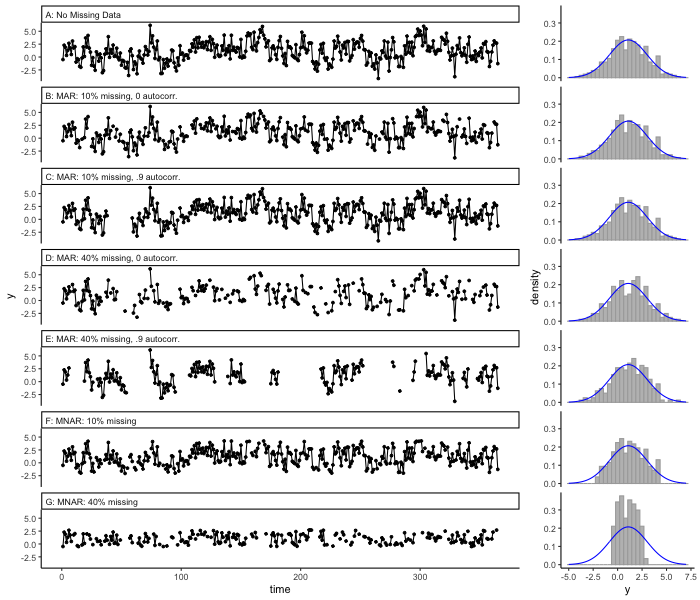
\includegraphics[width = 0.85\textwidth]{Figures/CompareMissingnessTypes_fig.png}
  %DIF <    \caption{}
   %DIF <   \label{fig:missingtypes}
%DIF <  \end{figure}
%DIFDELCMD < 

%DIFDELCMD < %%%
\DIFdelend %% Figure 1
\begin{figure}[h]
     \noindent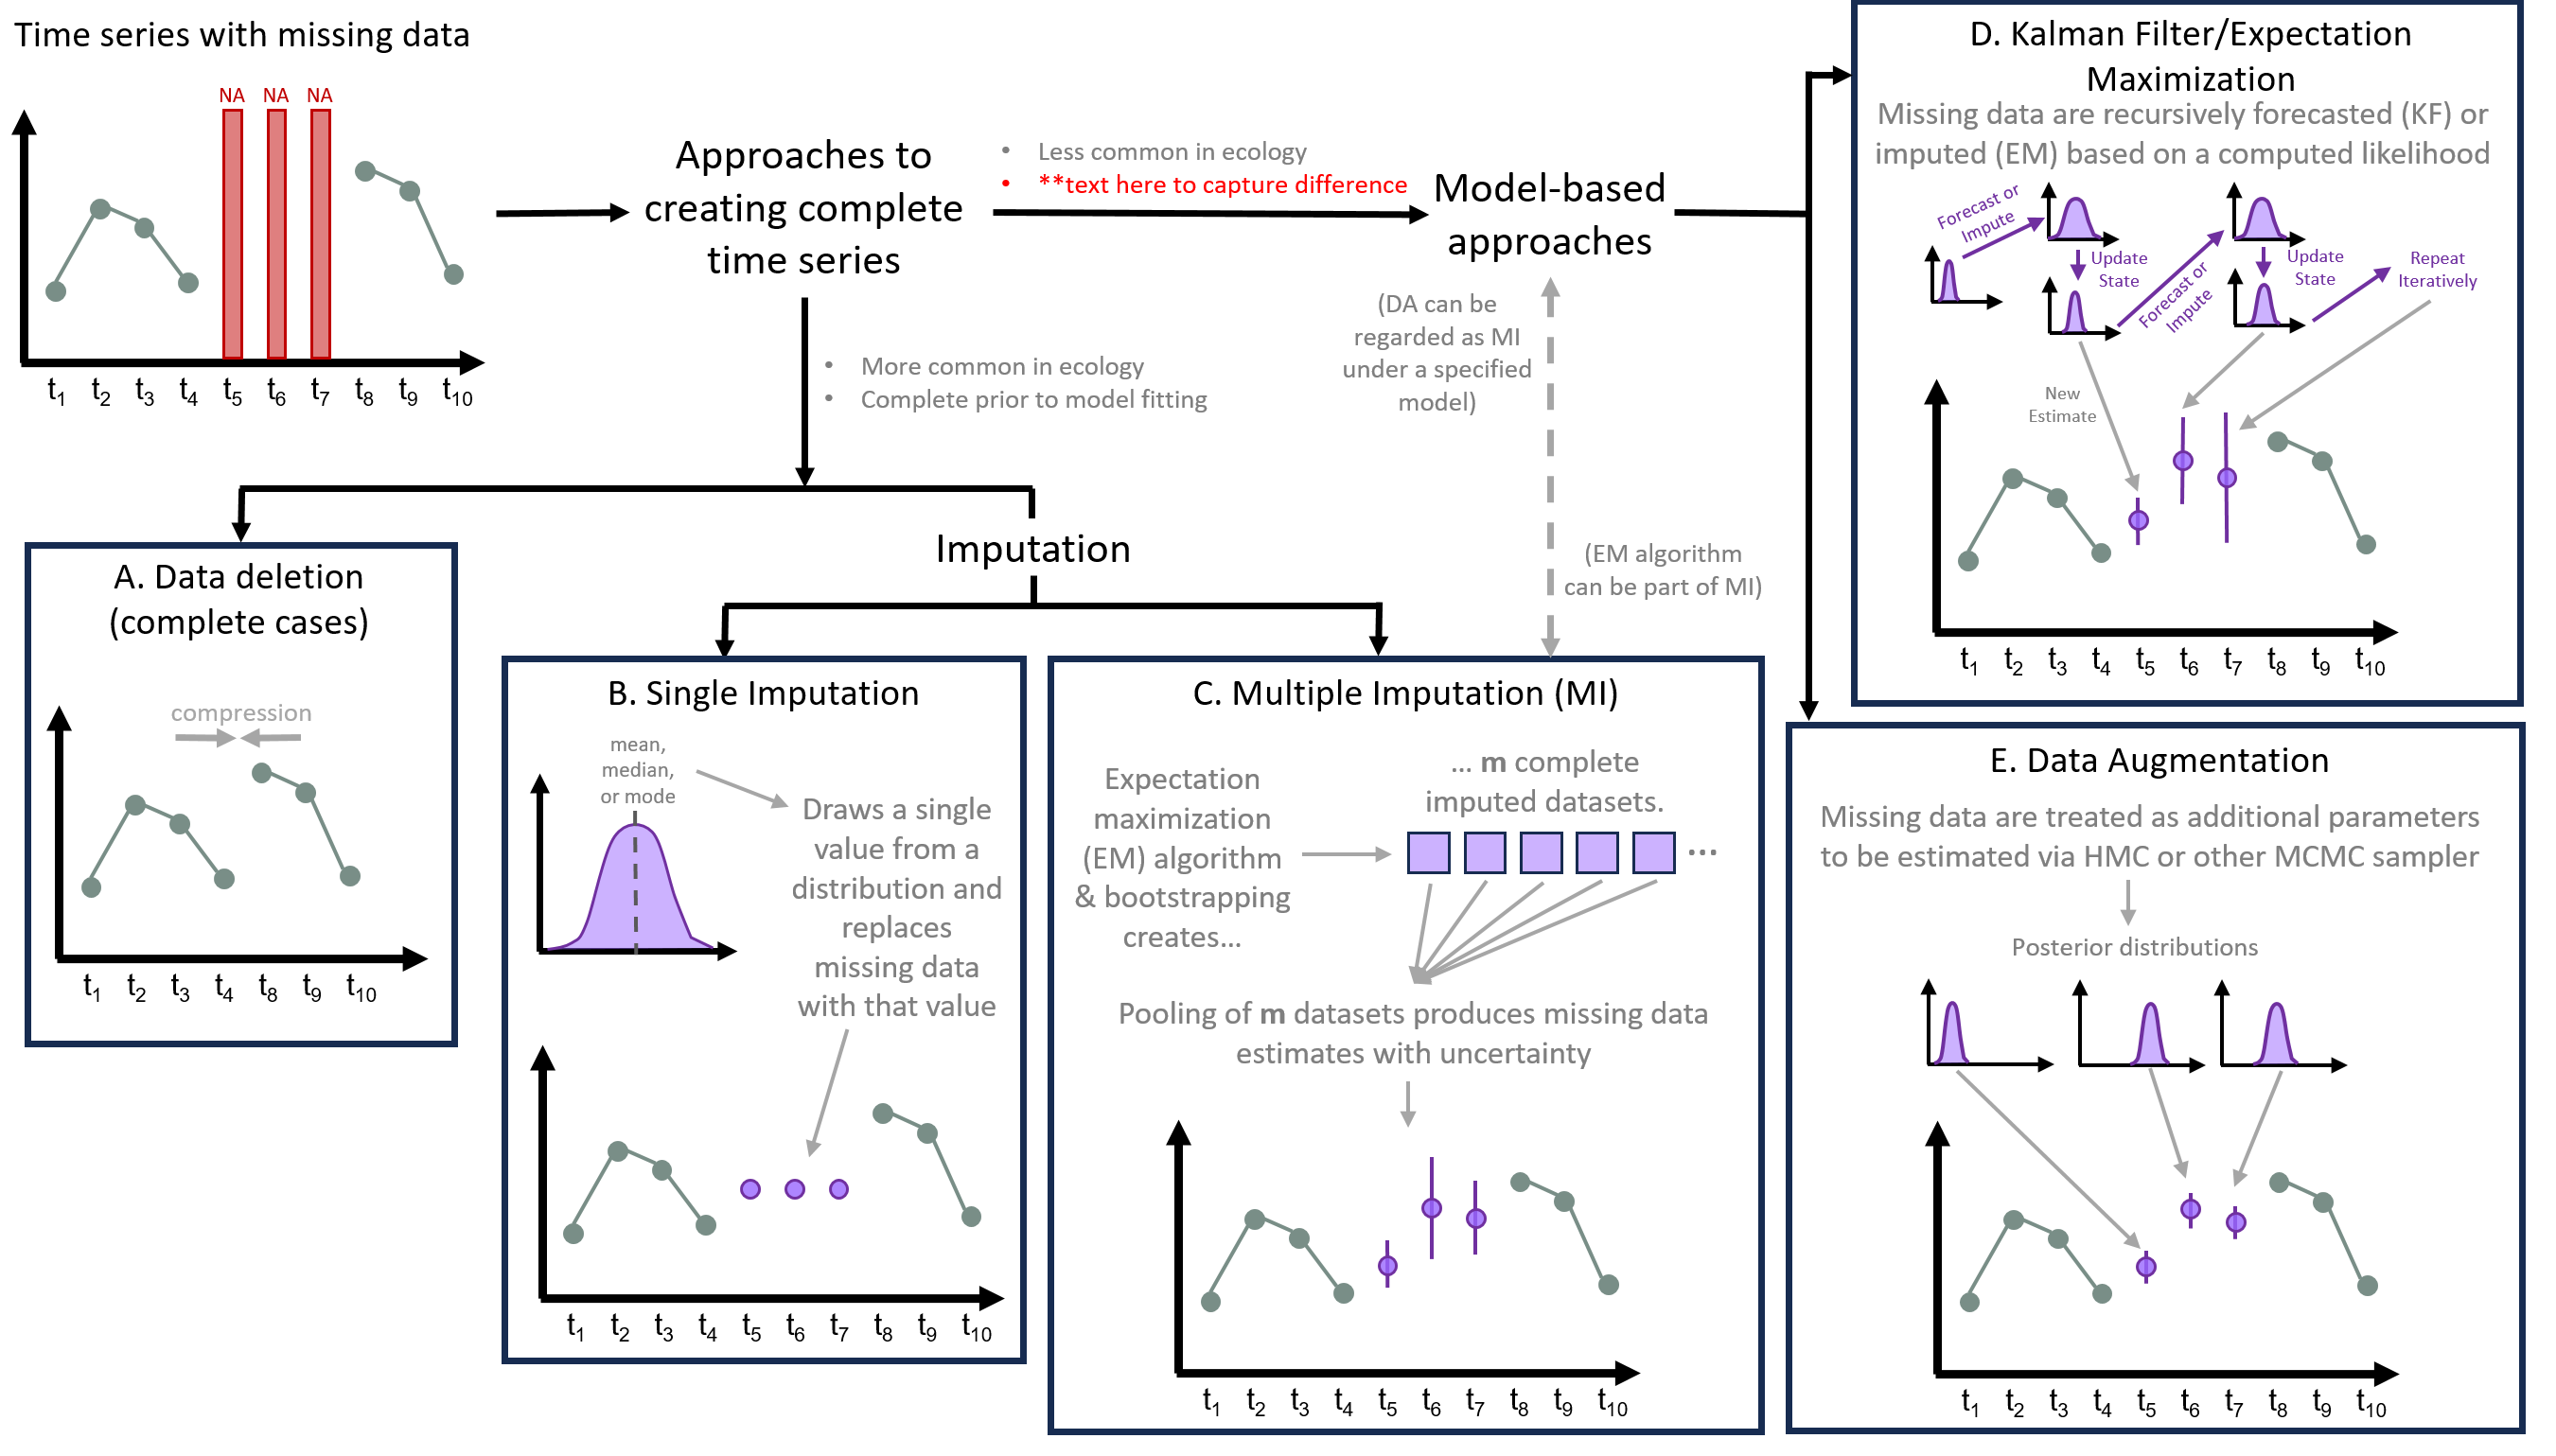
\includegraphics[width = .7\textwidth]{Figures/ConceptualFigure.png}
     \caption{}
     \label{fig:ConceptualFigure}
 \end{figure}

%% Figure 2
\begin{figure}
    \noindent\DIFdelbeginFL %DIFDELCMD < 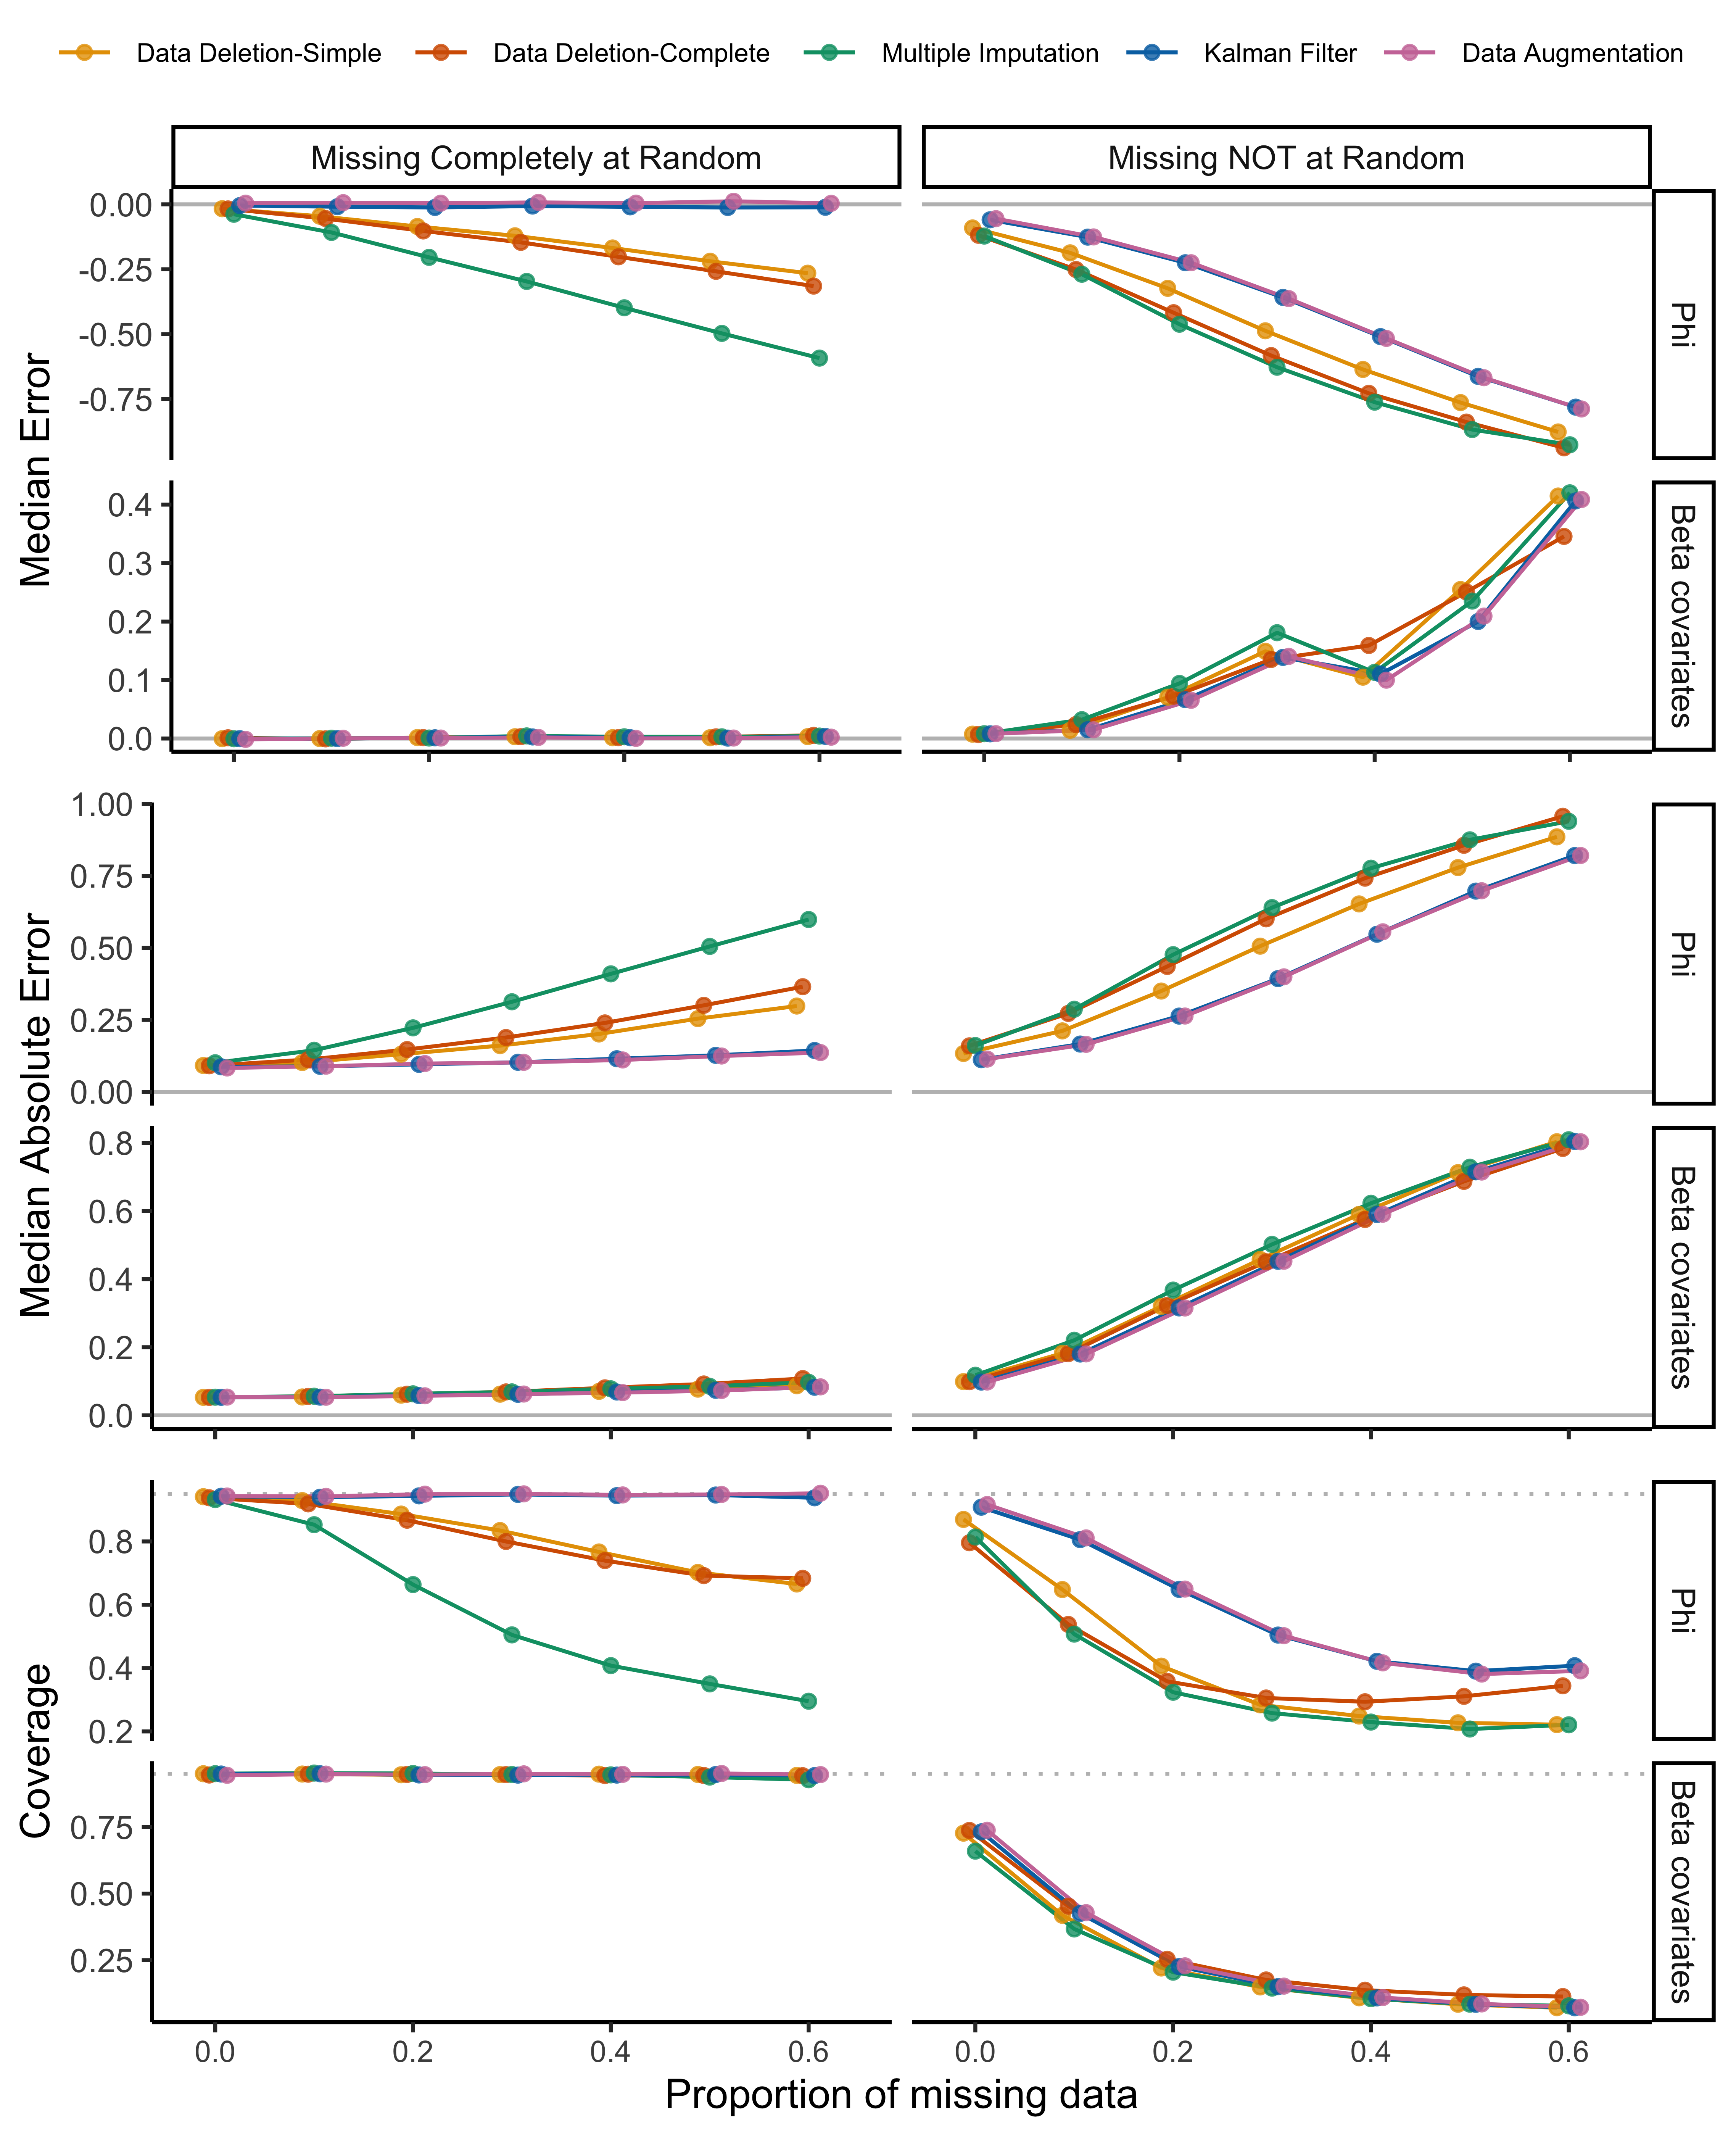
\includegraphics[width = .7\textwidth]{Figures/MockedUpFigures/parameterRecoveryGaussian_MARMNARlong.png}
%DIFDELCMD <     %%%
\DIFdelendFL \DIFaddbeginFL 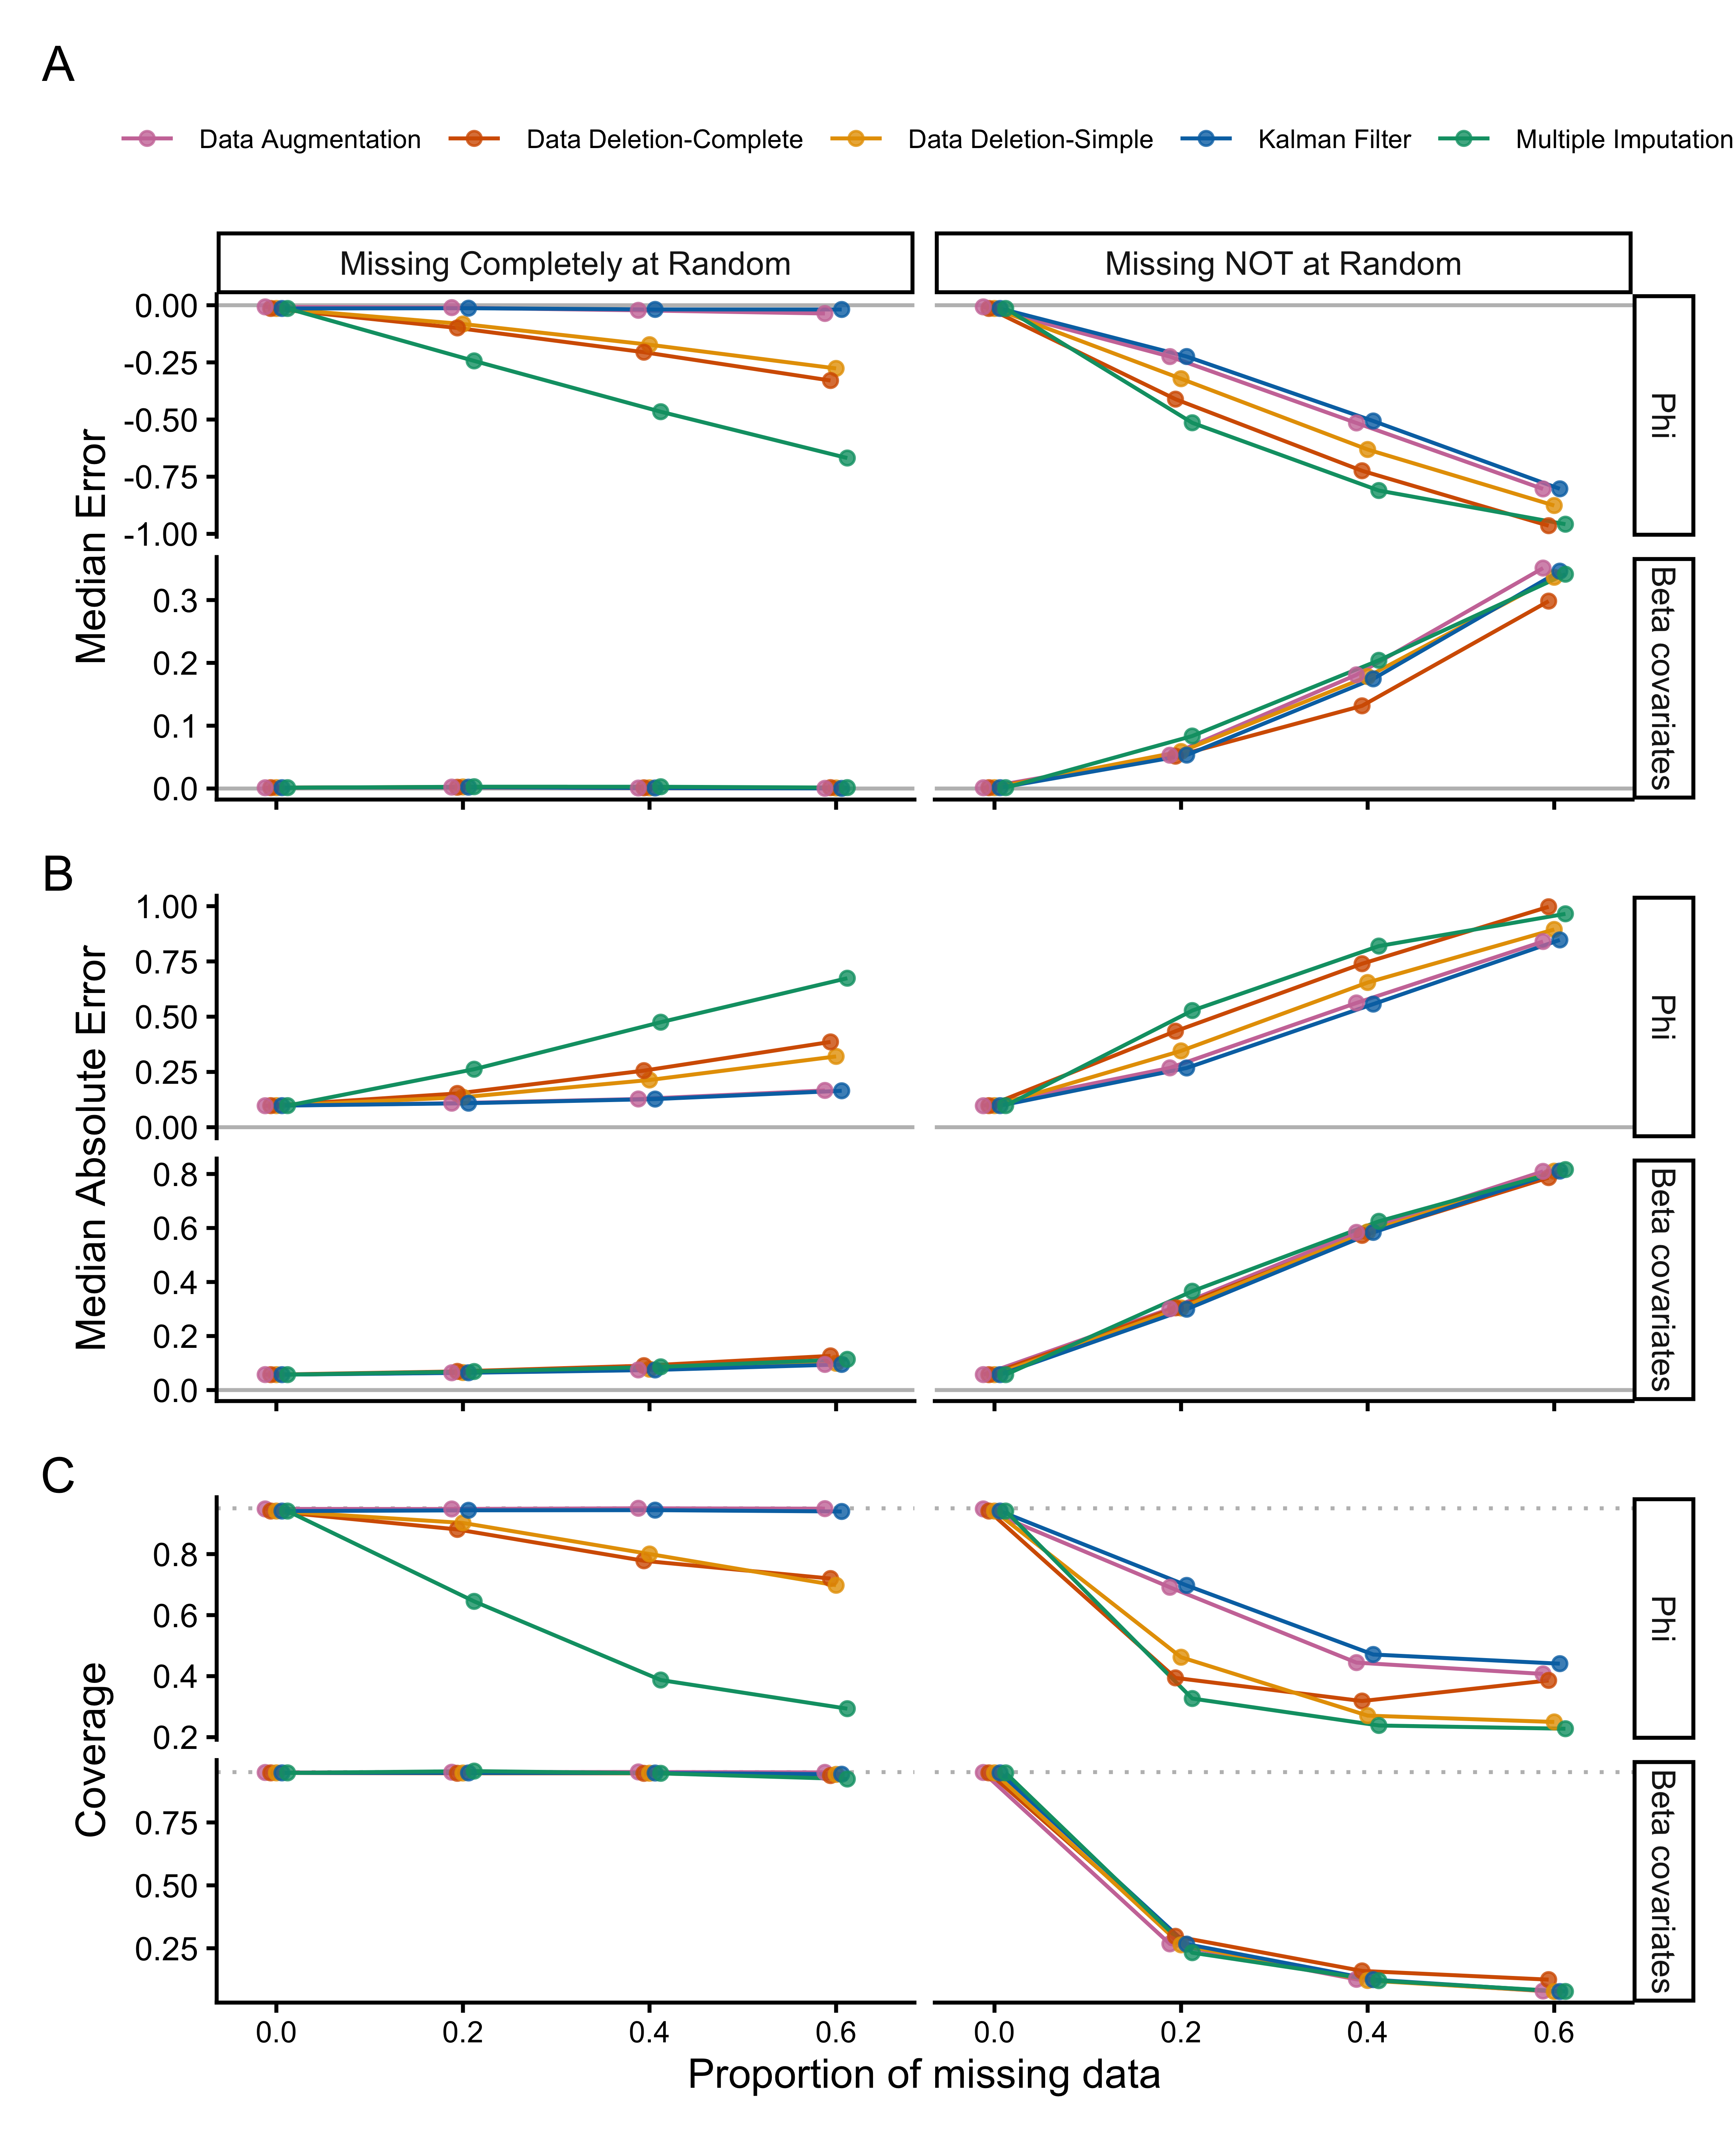
\includegraphics[width = .7\textwidth]{Figures/NewFiguresForRevision/simGauss_paramRecovery.png}
    %DIF > MockedUpFigures/parameterRecoveryGaussian_MARMNARlong.png}
    \DIFaddendFL \caption{} 

    \label{fig:ParamRec_Gauss}
\end{figure}

\clearpage

%% Figure 3
\begin{figure}
    \noindent\DIFdelbeginFL %DIFDELCMD < 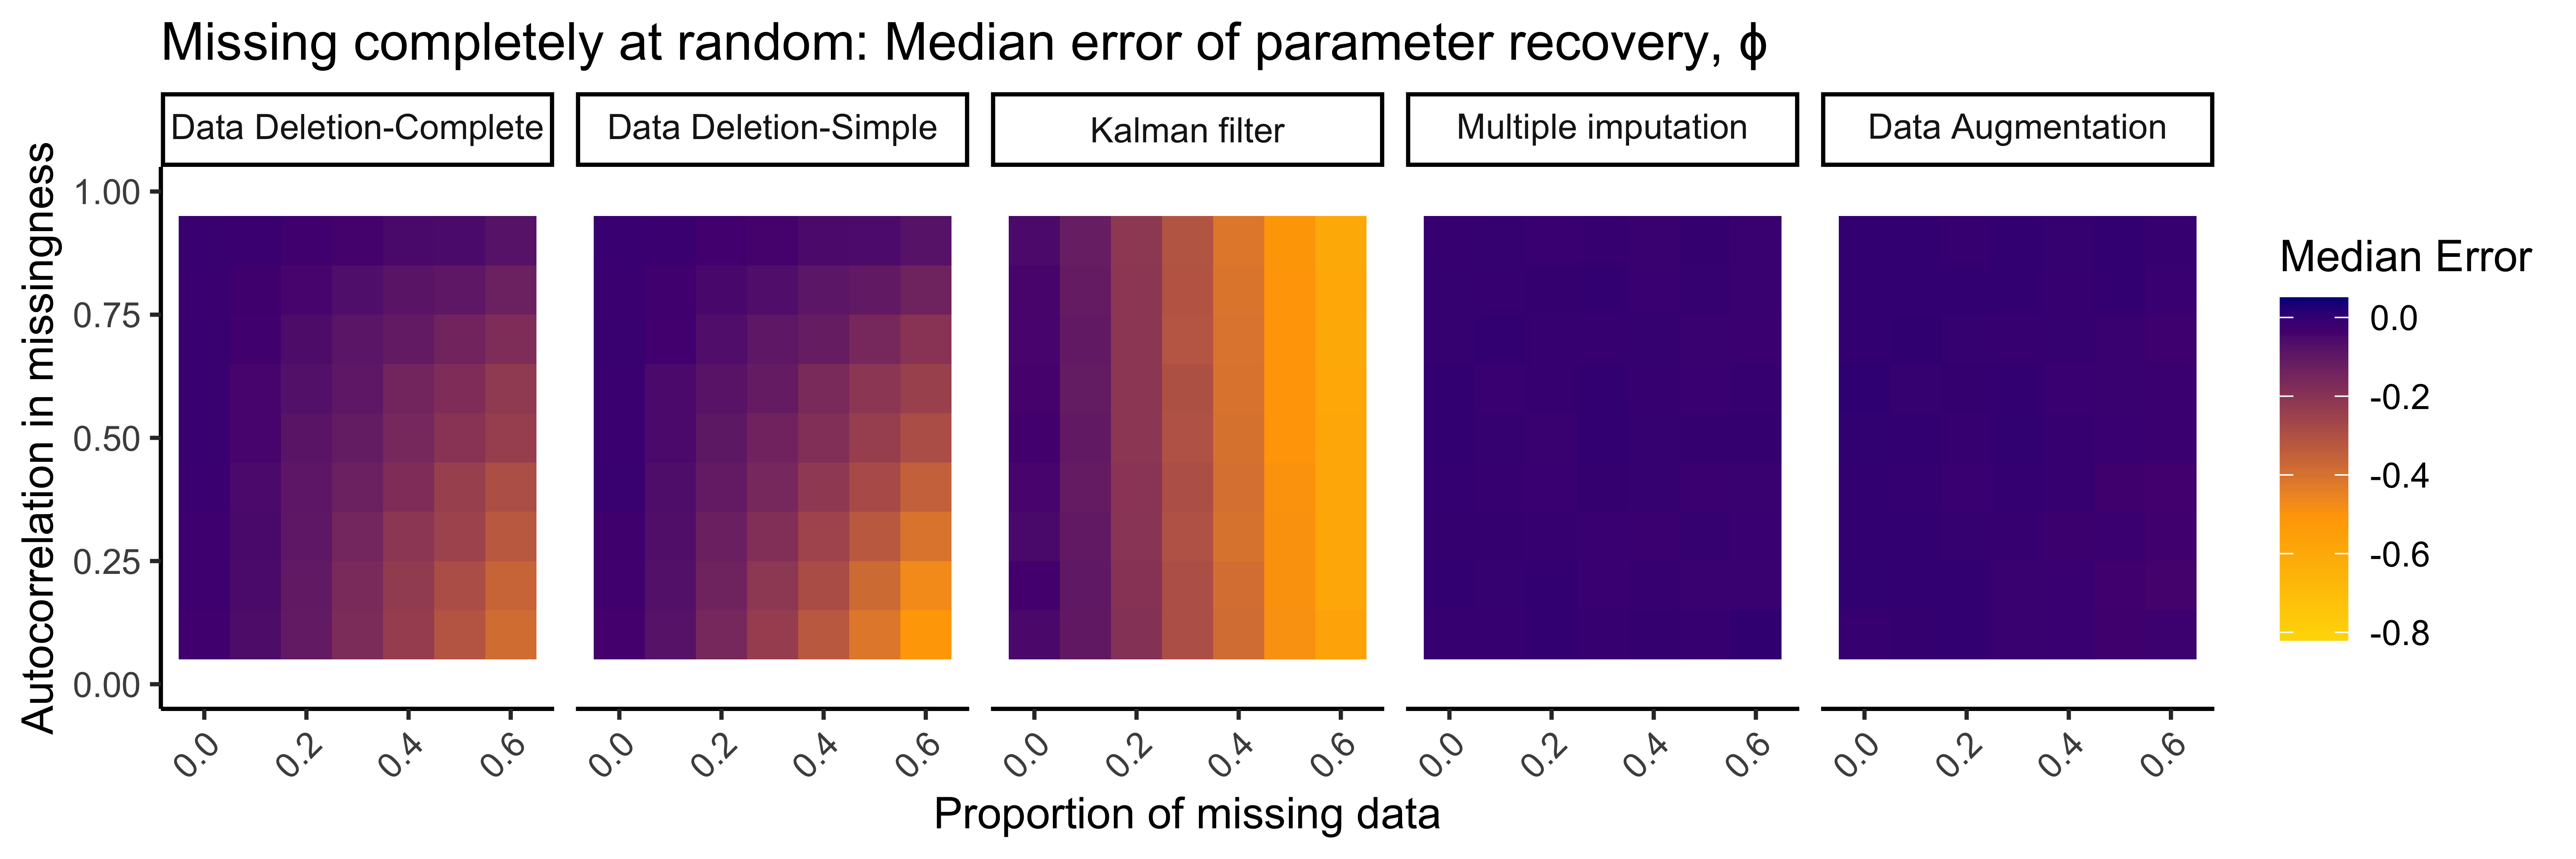
\includegraphics[width = \textwidth]{Figures/MockedUpFigures/heatmap_GaussianMCAR_justPhi.png}
%DIFDELCMD < %%%
\DIFdelendFL \DIFaddbeginFL 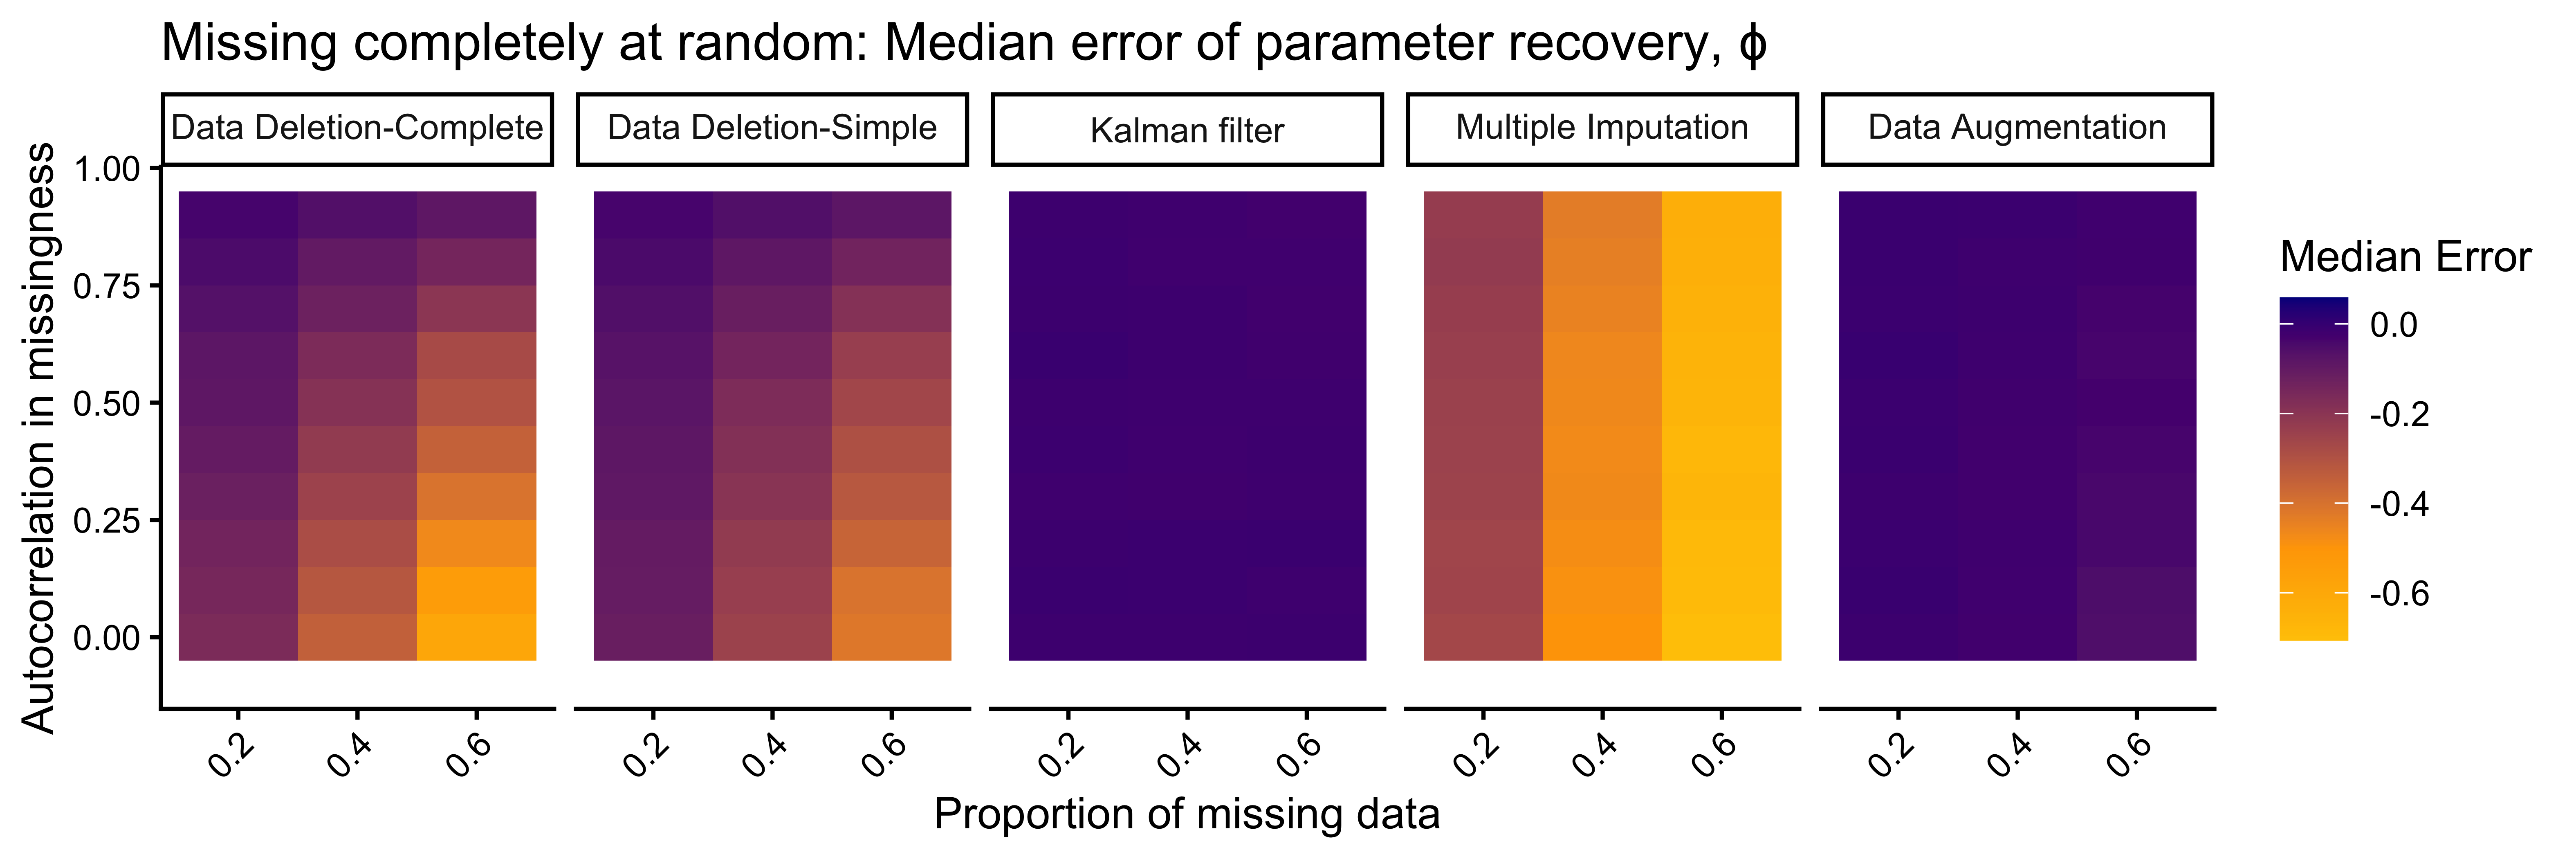
\includegraphics[width = \textwidth]{Figures/NewFiguresForRevision/simGaussData_MCAR_heatmap_justPhi.png.png}
    %DIF > {Figures/MockedUpFigures/heatmap_GaussianMCAR_justPhi.png}
\DIFaddendFL 

    \caption{}

    \label{fig:heatMap_gauss_MAR}
\end{figure}

\pagebreak

%% Figure 4
\begin{figure}
    \centering
    \noindent\DIFdelbeginFL %DIFDELCMD < 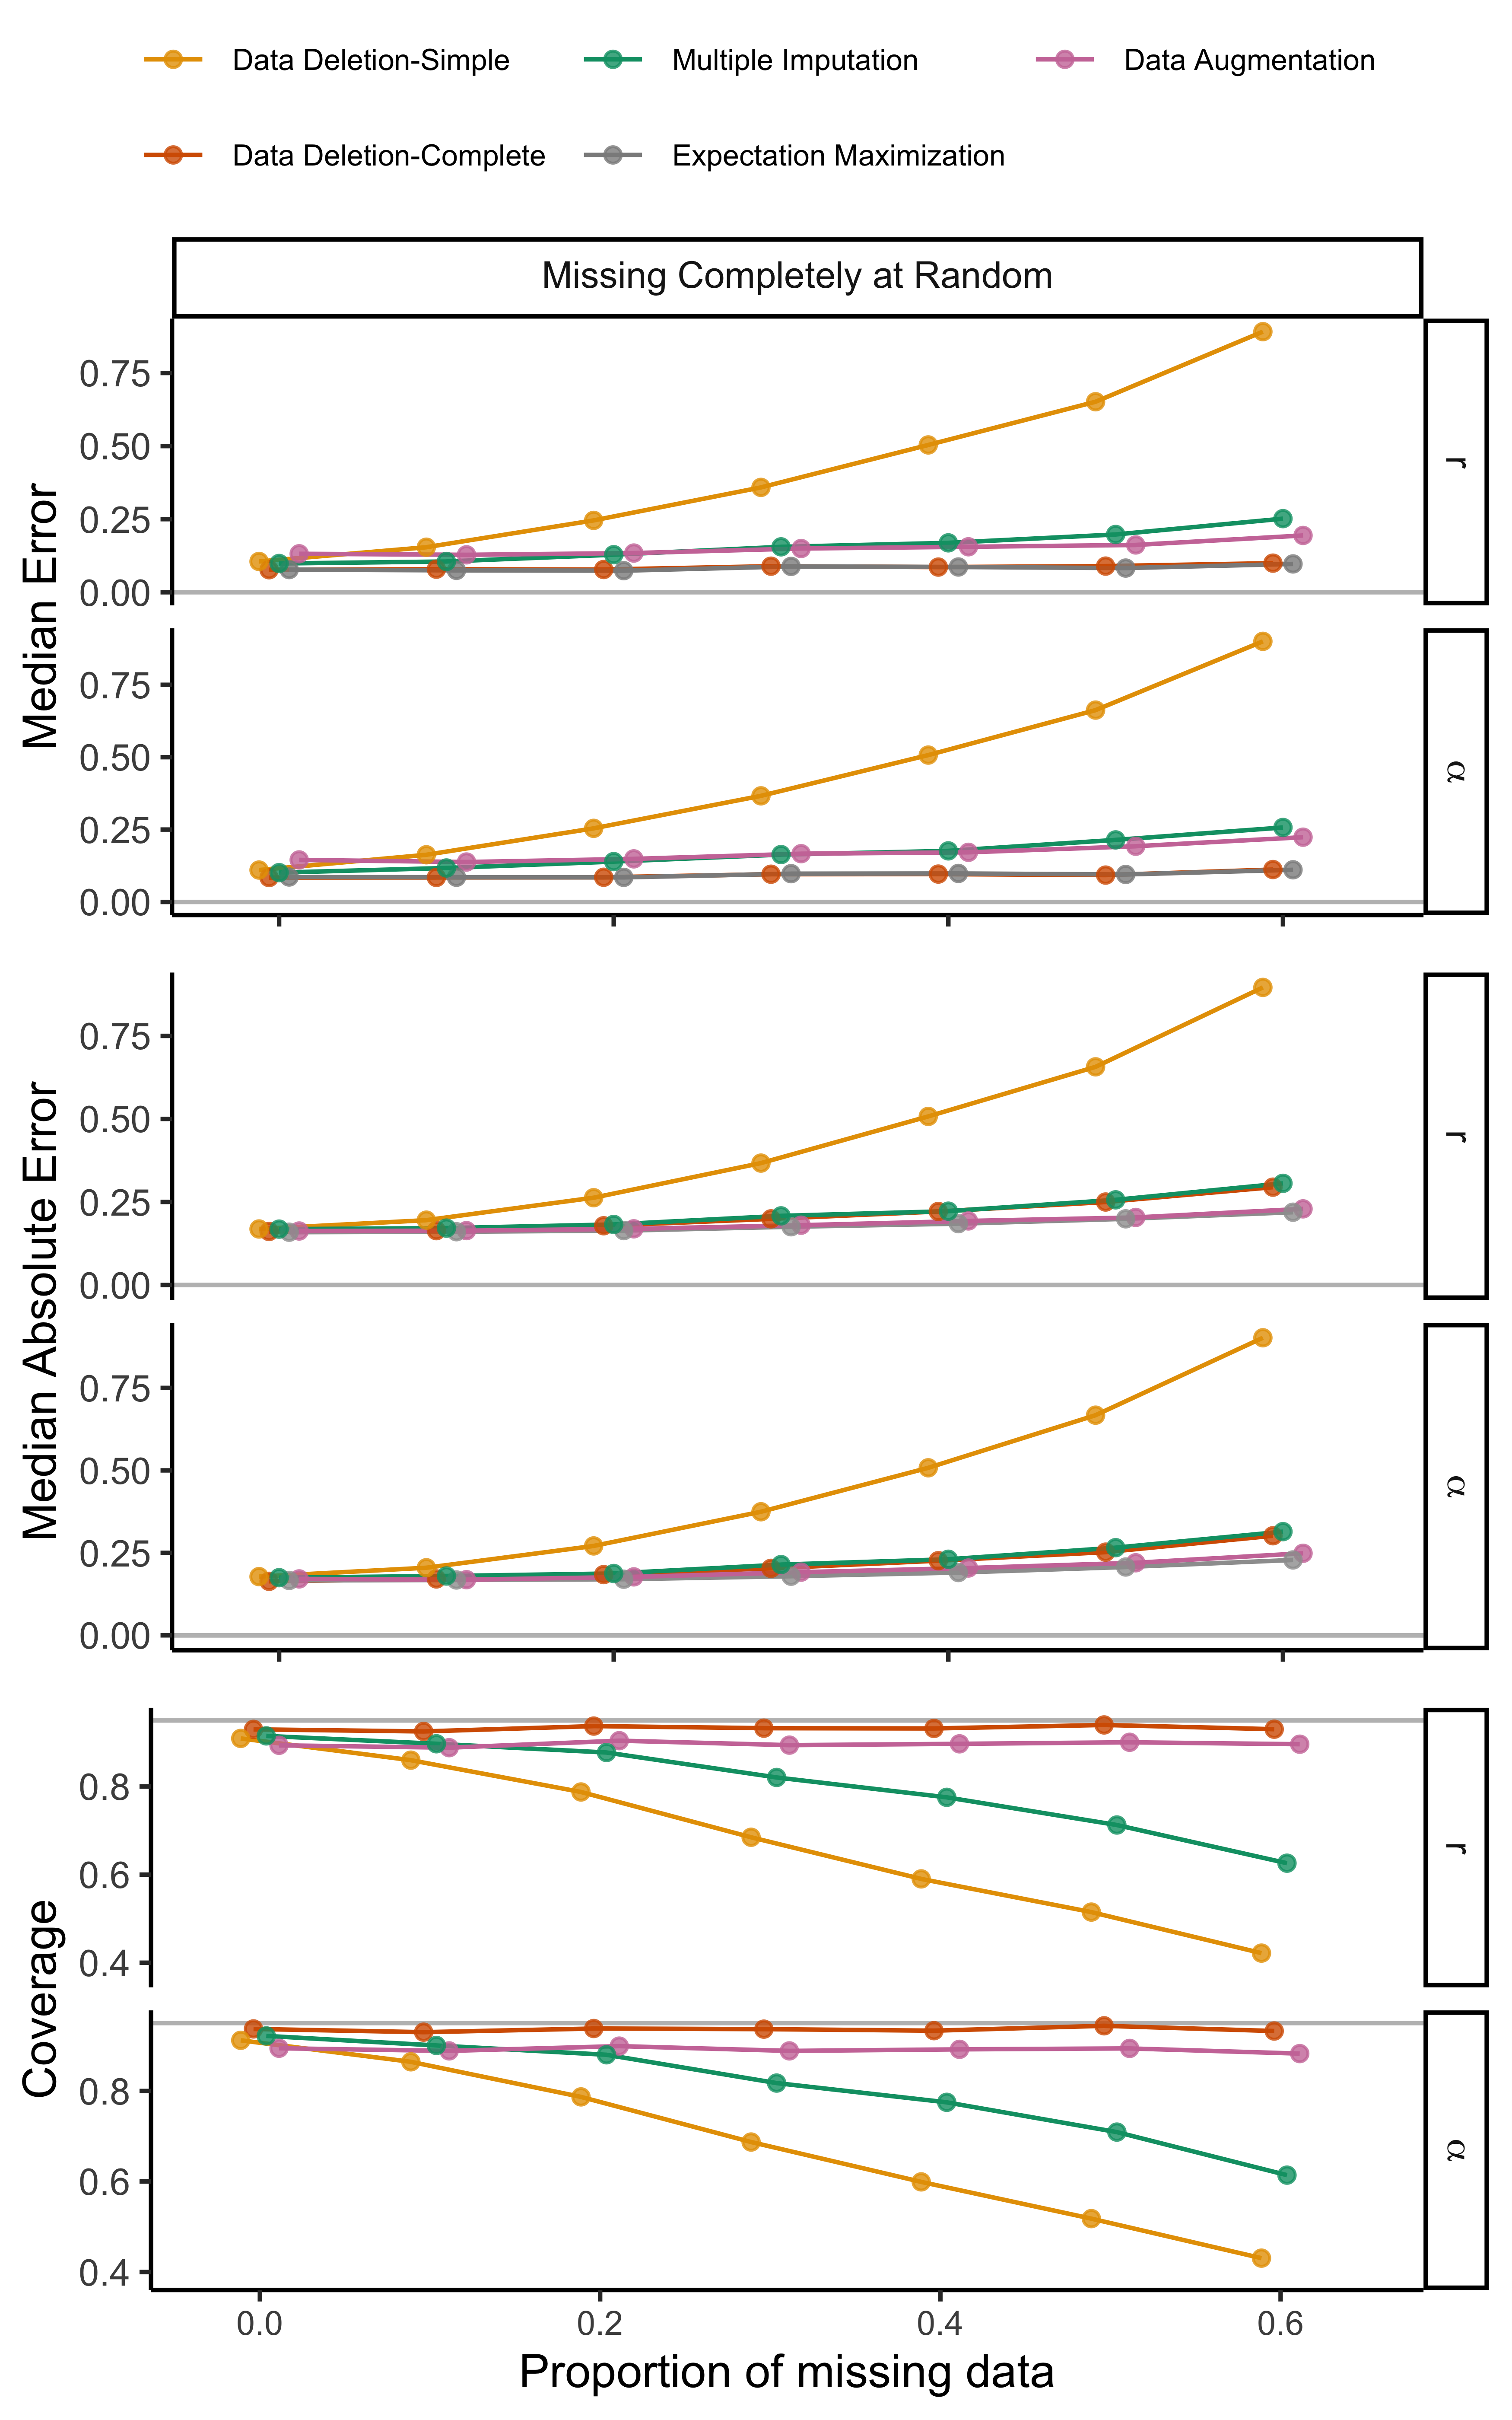
\includegraphics[width = 0.7\textwidth]{Figures/MockedUpFigures/parameterRecoveryPoisson_MCARlong.png}
%DIFDELCMD <     %%%
\DIFdelendFL \DIFaddbeginFL 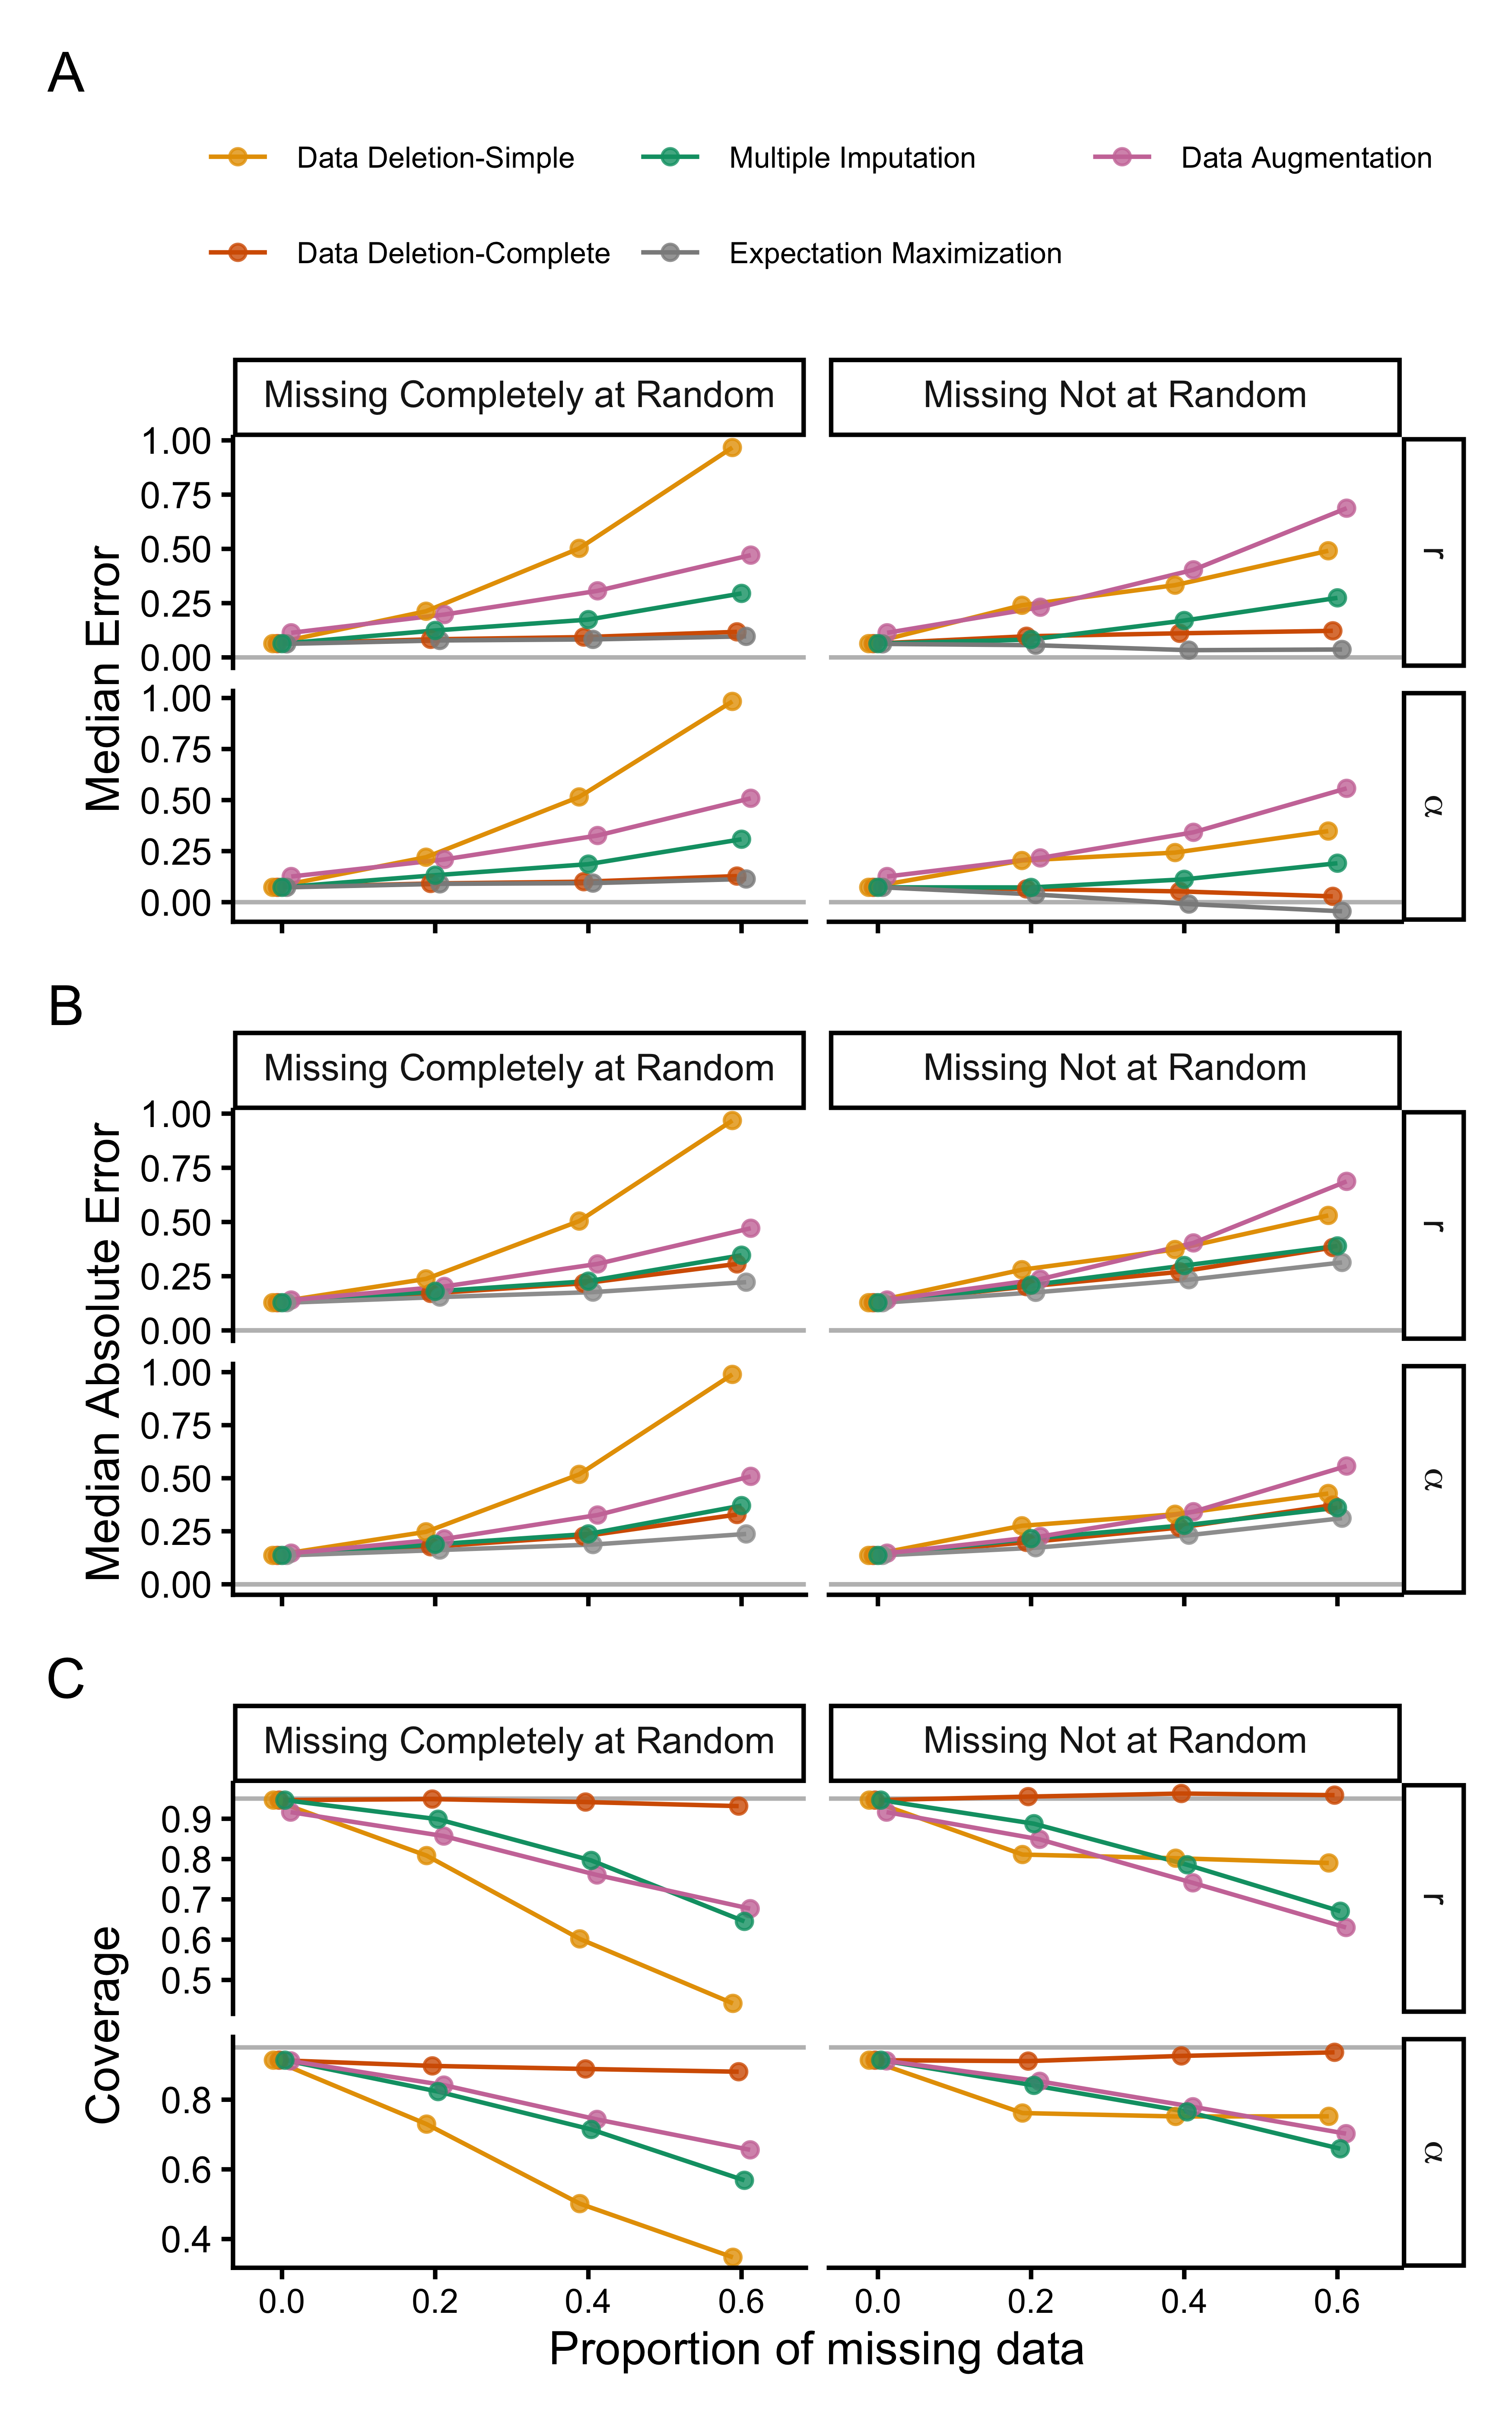
\includegraphics[width = 0.7\textwidth]{Figures/NewFiguresForRevision/simPoiss_paramRecovery.png}
    %DIF > {Figures/MockedUpFigures/parameterRecoveryPoisson_MCARlong.png}
    \DIFaddendFL \caption{}

    \label{fig:ParamRec_Pois}
\end{figure}

%% Figure 5
\begin{figure}
    \centering
    \noindent\DIFdelbeginFL %DIFDELCMD < 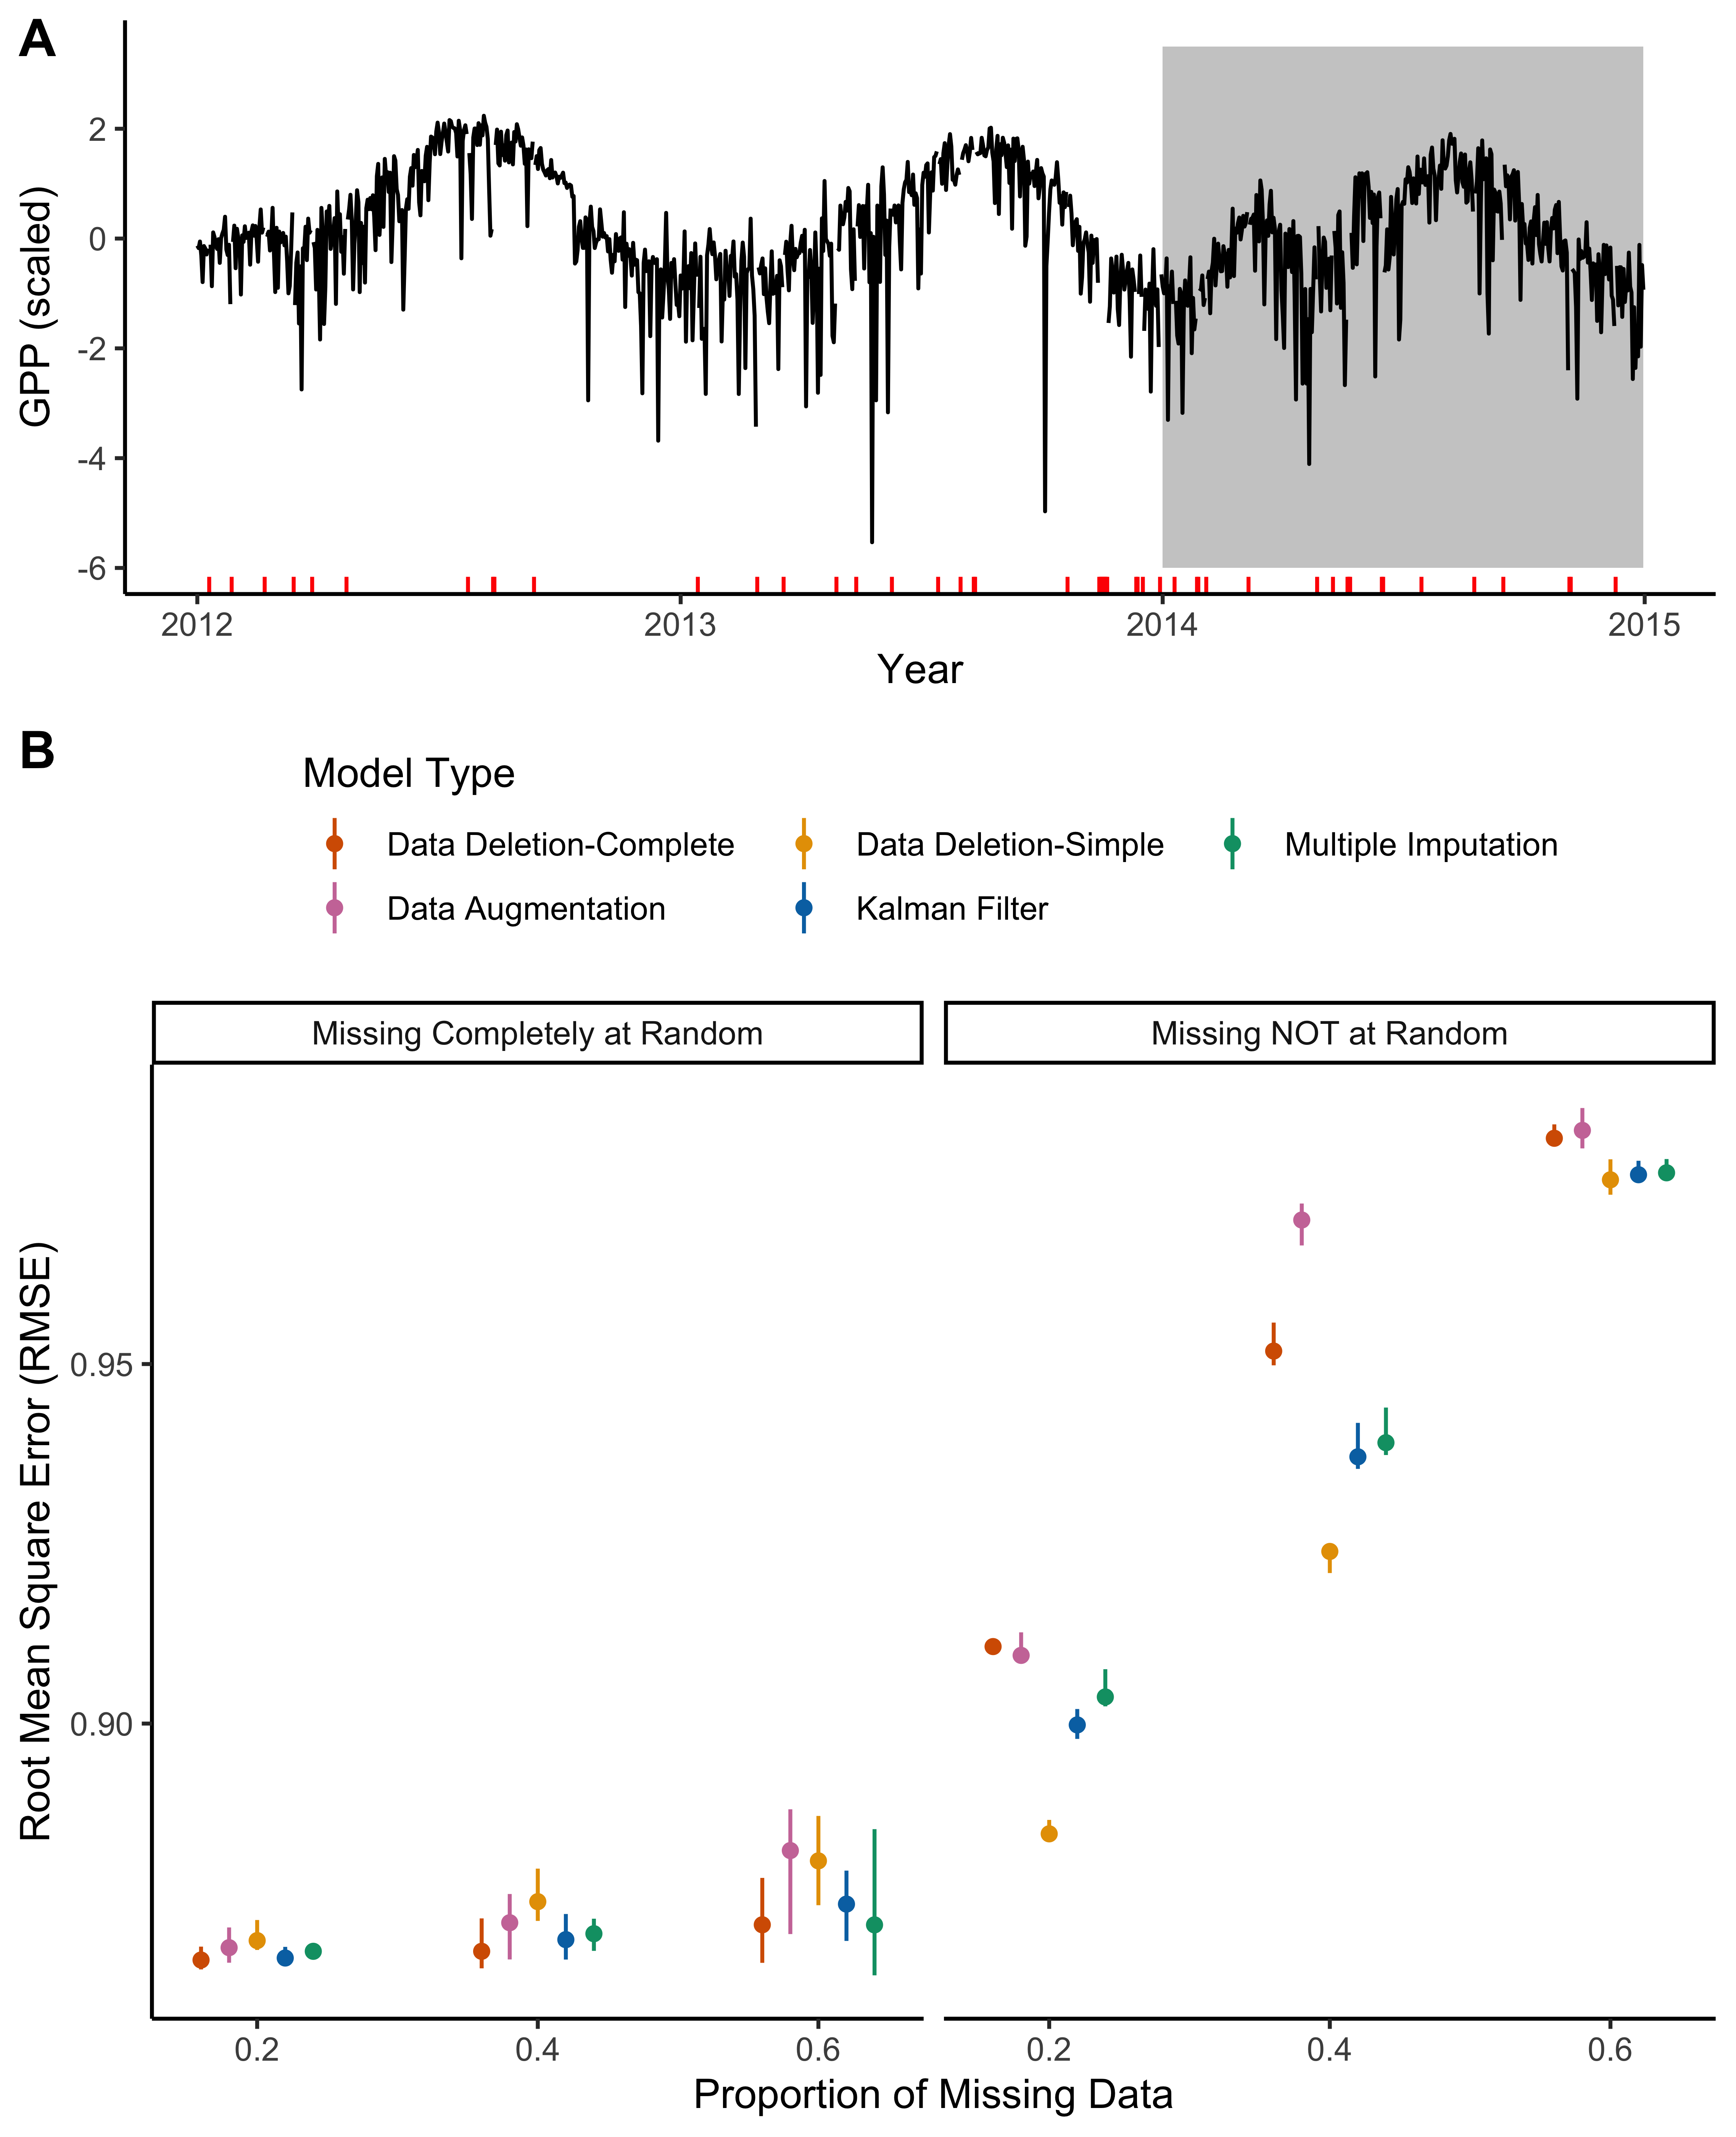
\includegraphics[width = 0.85\textwidth]{Figures/MockedUpFigures/RMSE_FullFigure_NoLineWithErrorBar_gaussian_auSable.png}
%DIFDELCMD < %%%
\DIFdelendFL \DIFaddbeginFL 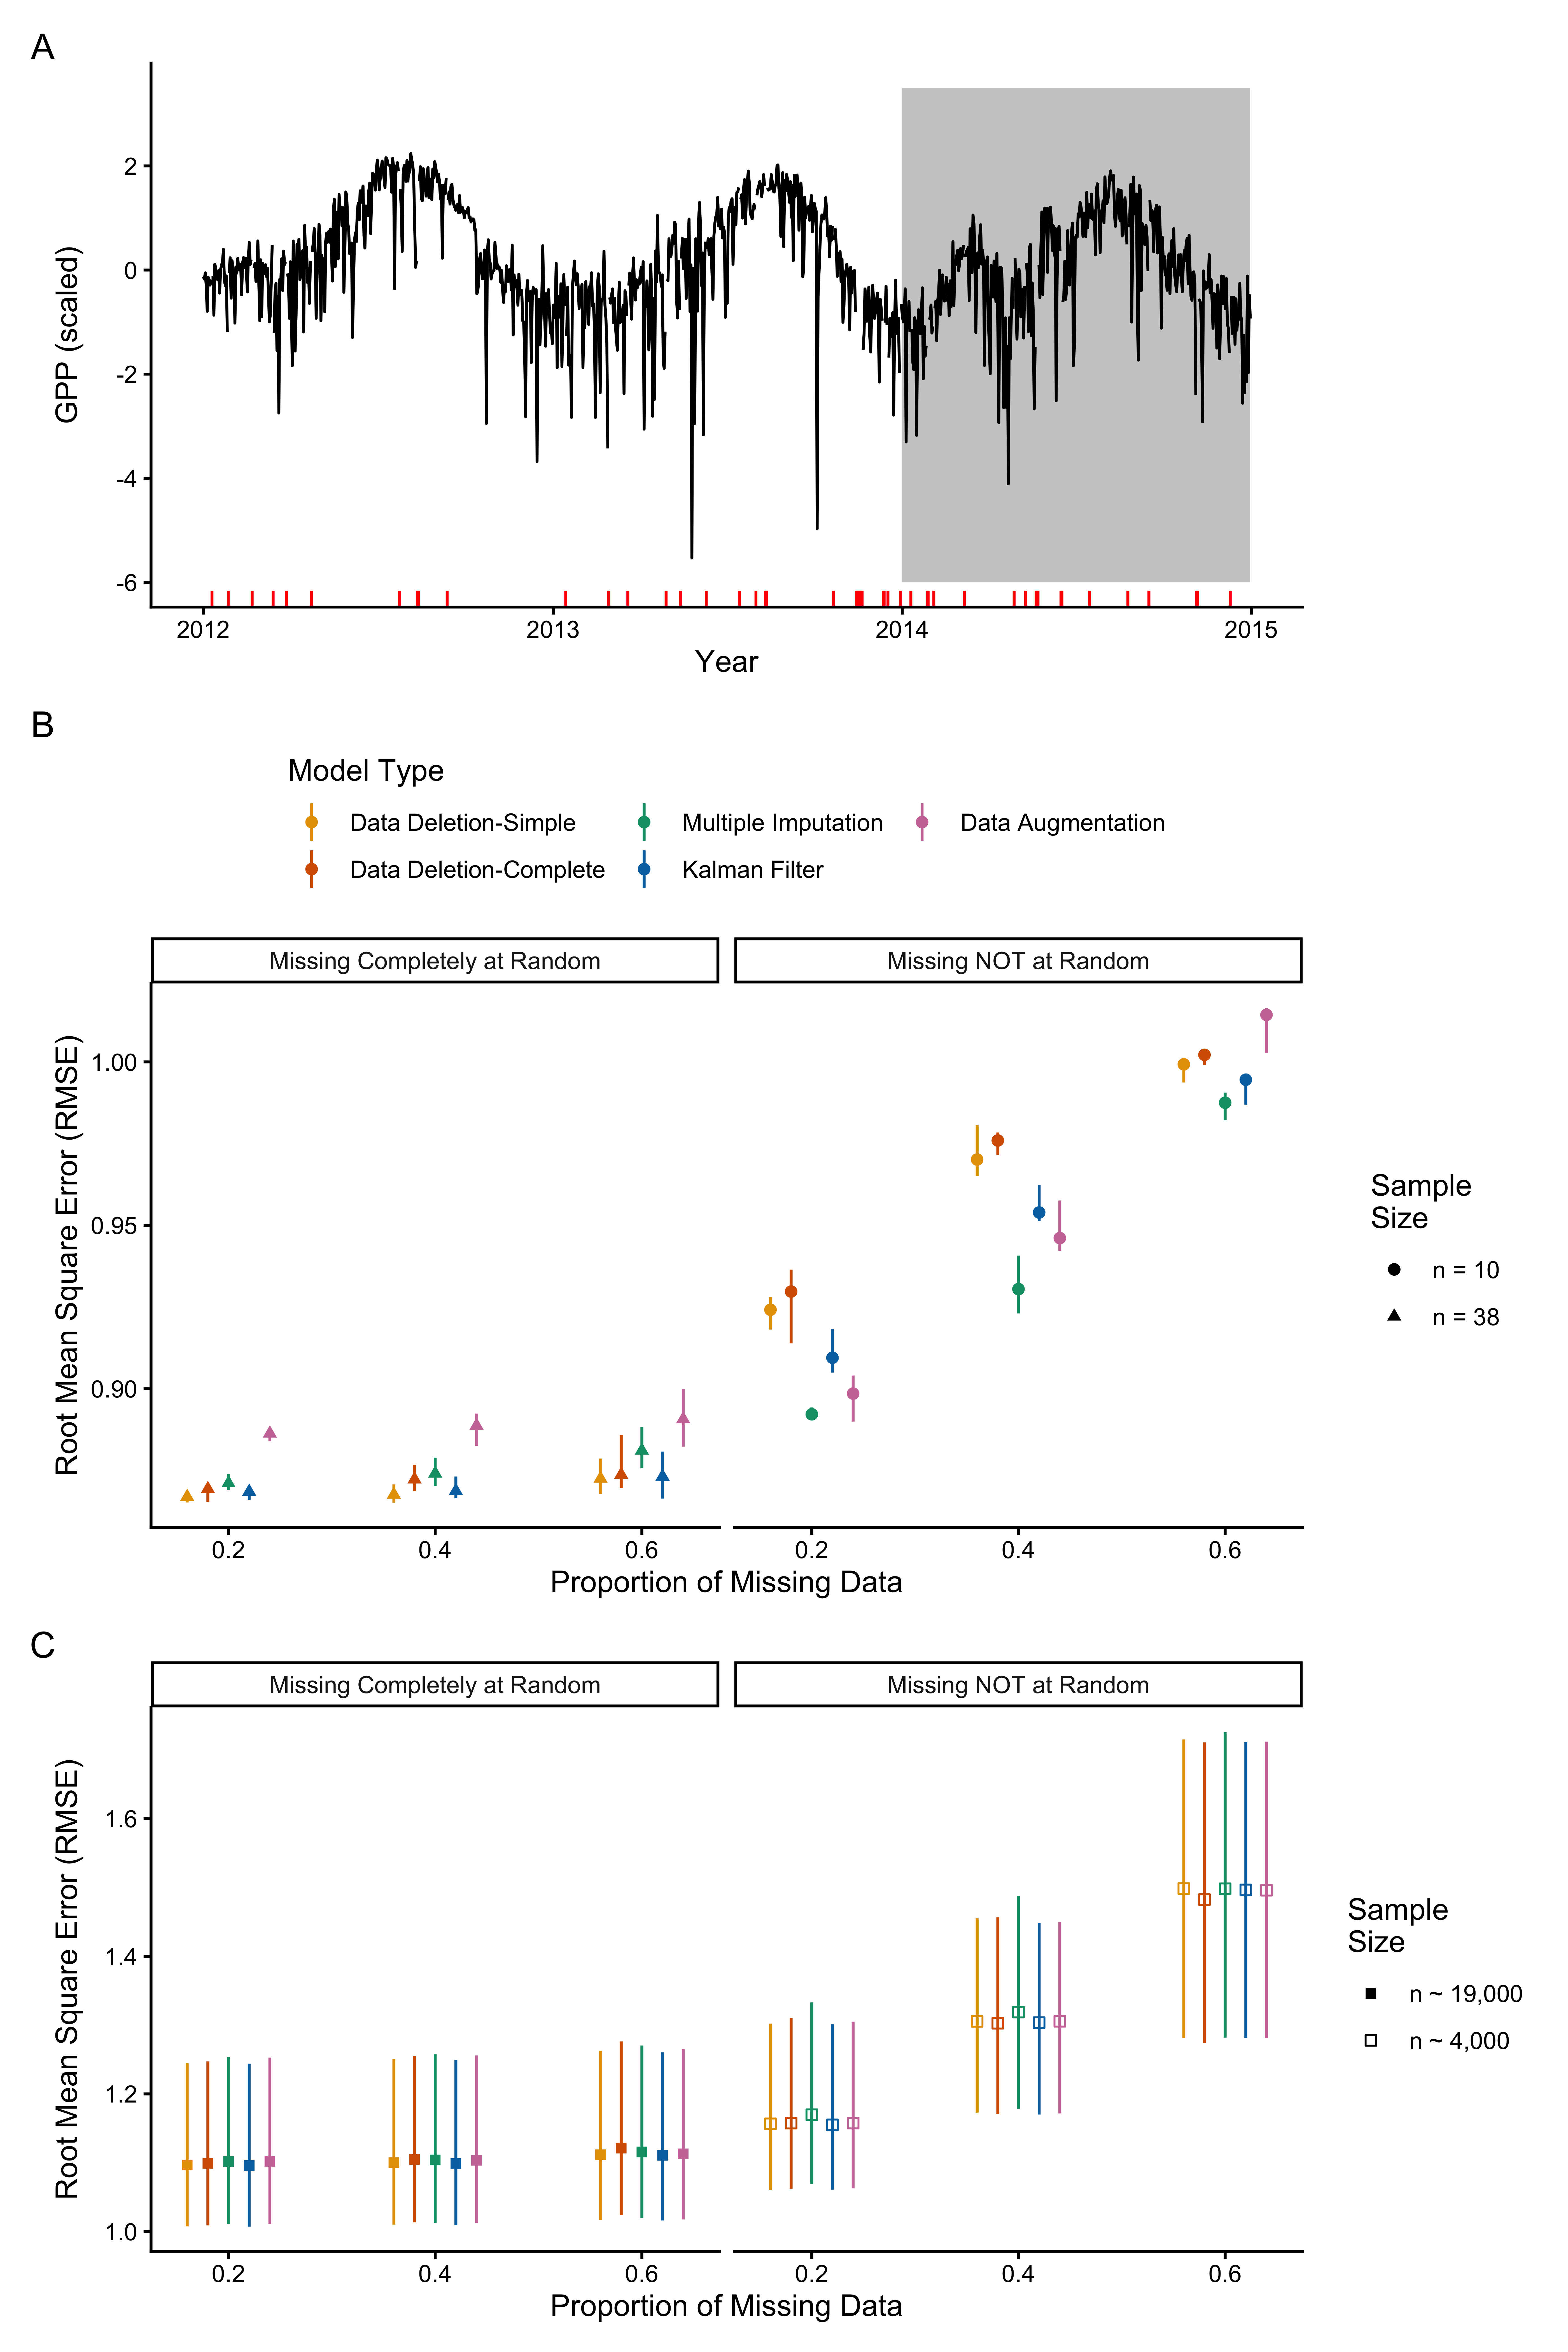
\includegraphics[width = 0.85\textwidth]{Figures/NewFiguresForRevision/RMSE_forAllGaussData.png}
    %DIF > {Figures/MockedUpFigures/RMSE_FullFigure_NoLineWithErrorBar_gaussian_auSable.png}
\DIFaddendFL 

    \caption{}

    \label{fig:RMSE_Gaus}
\end{figure}

%% Figure 6
\begin{figure}
    \noindent\DIFdelbeginFL %DIFDELCMD < 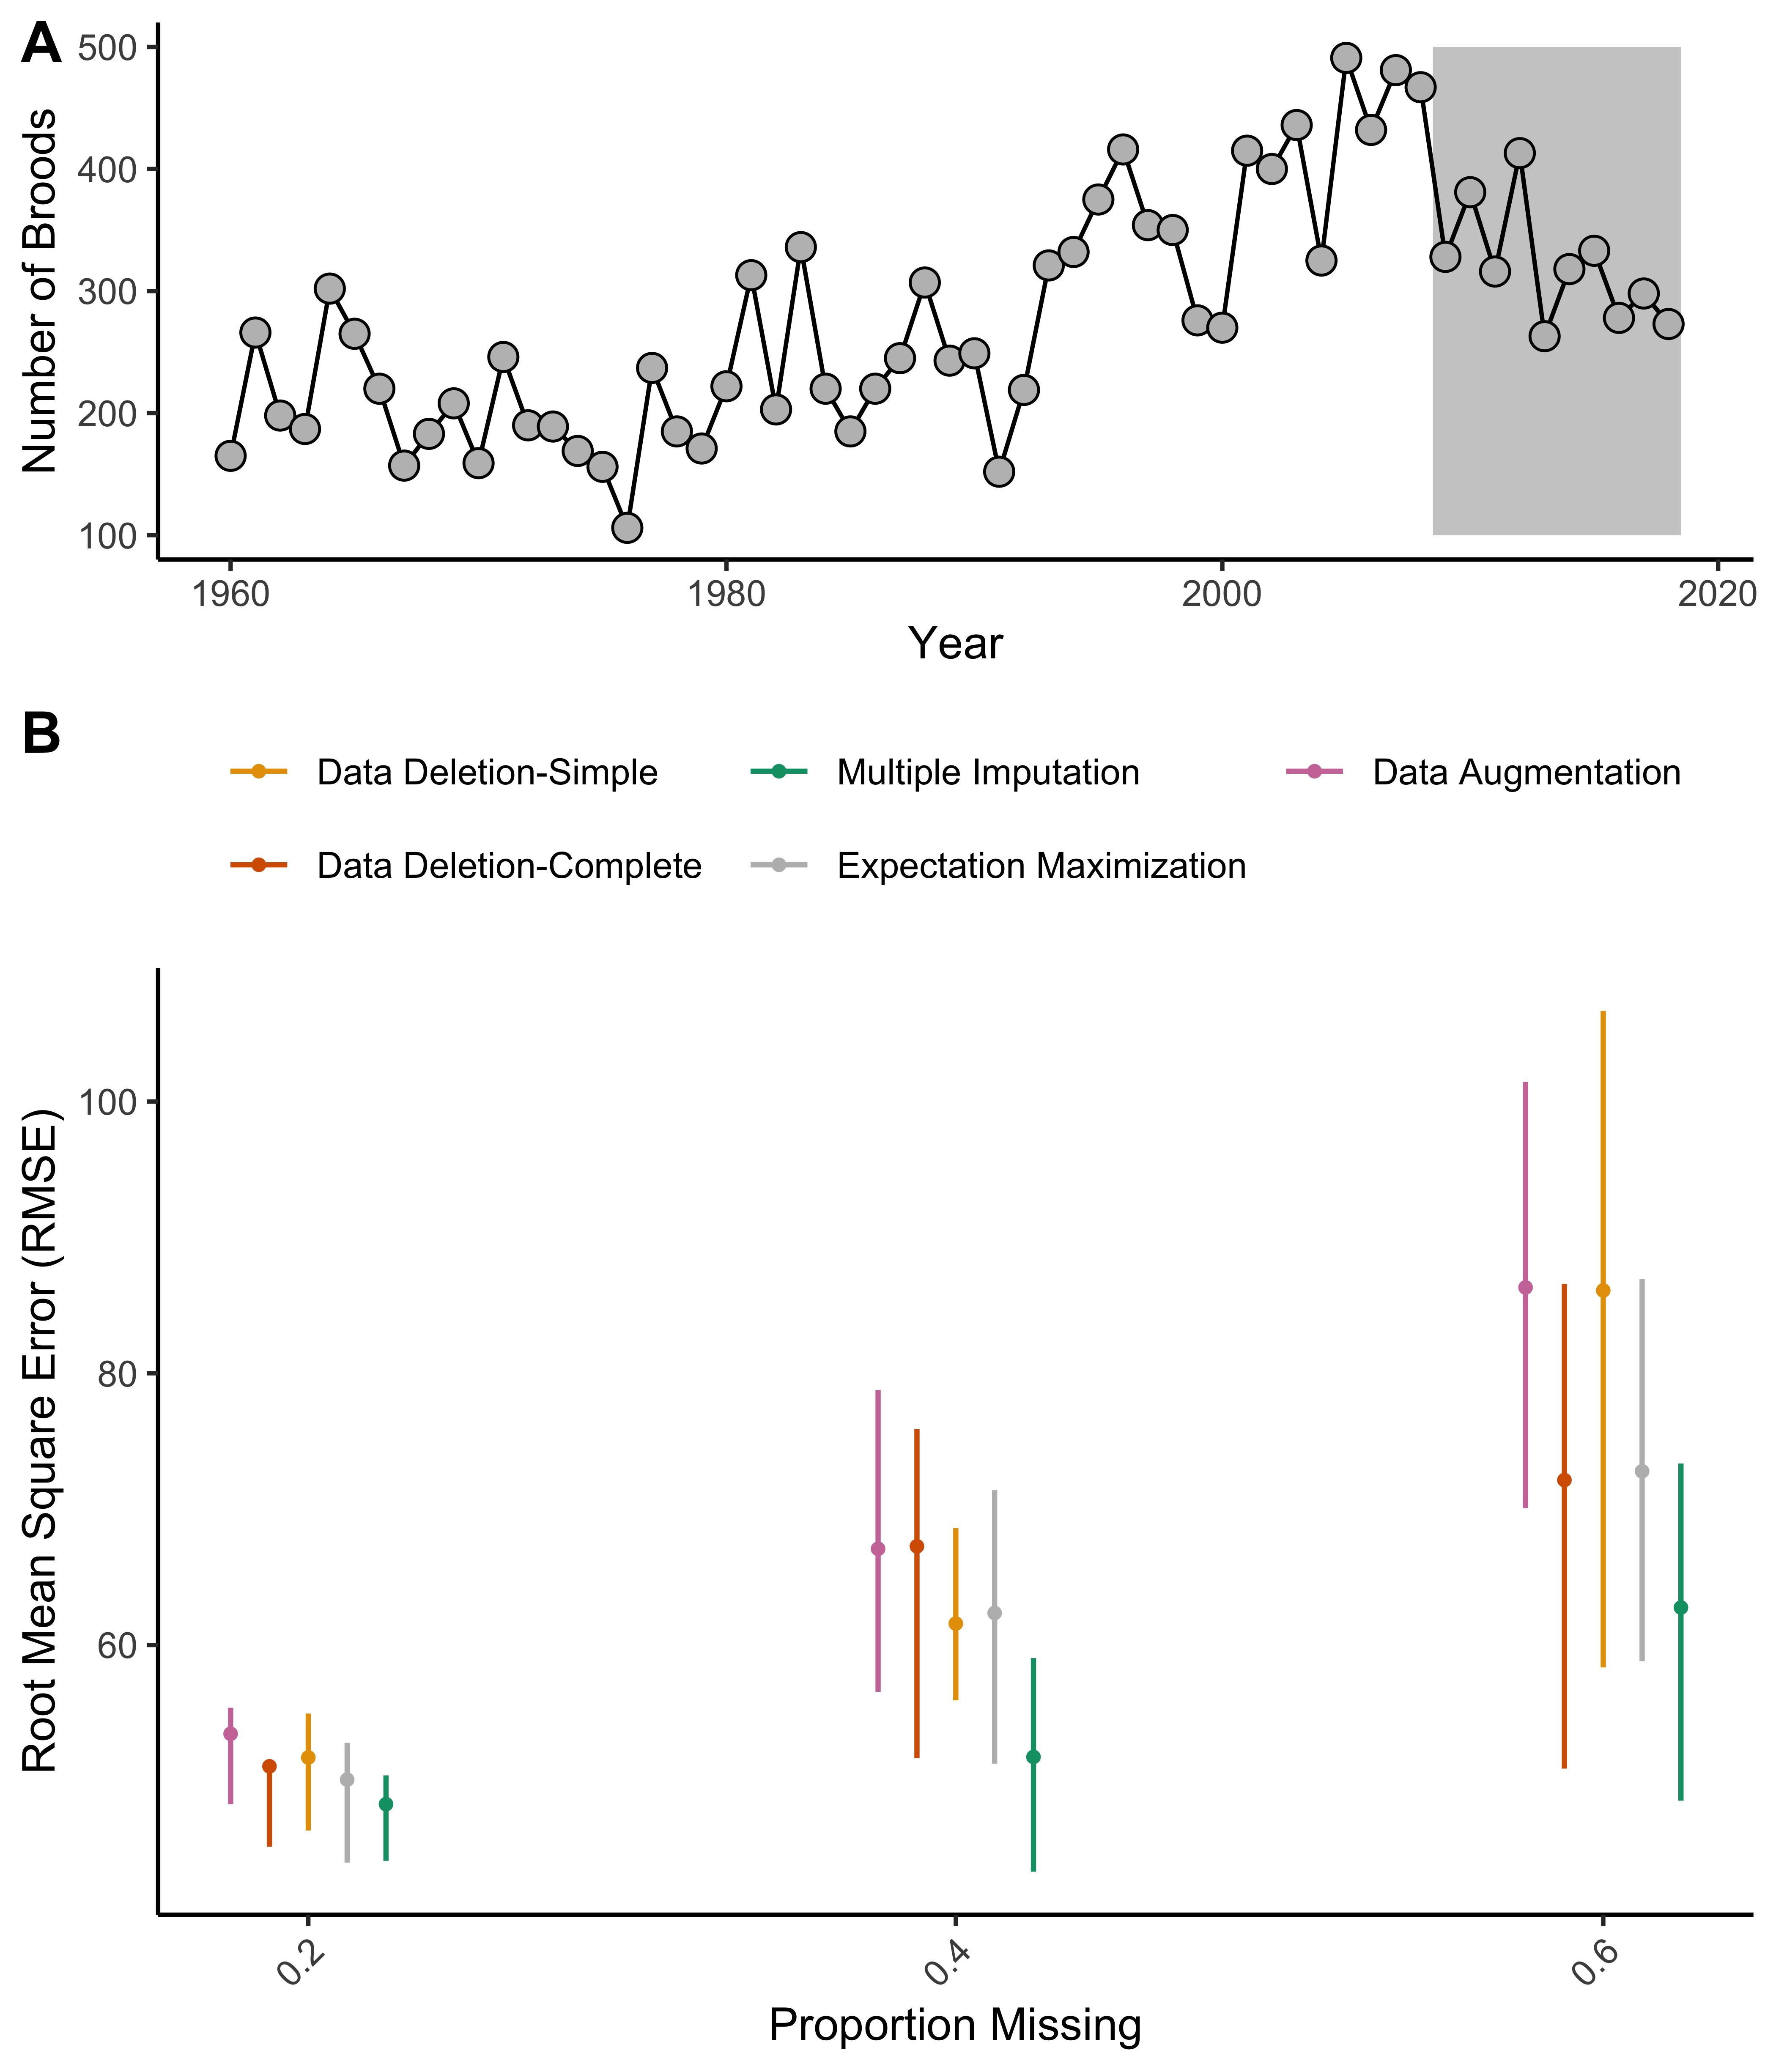
\includegraphics[width = \textwidth]{Figures/MockedUpFigures/RMSE_pois_combined.png}
%DIFDELCMD <     %%%
\DIFdelendFL \DIFaddbeginFL 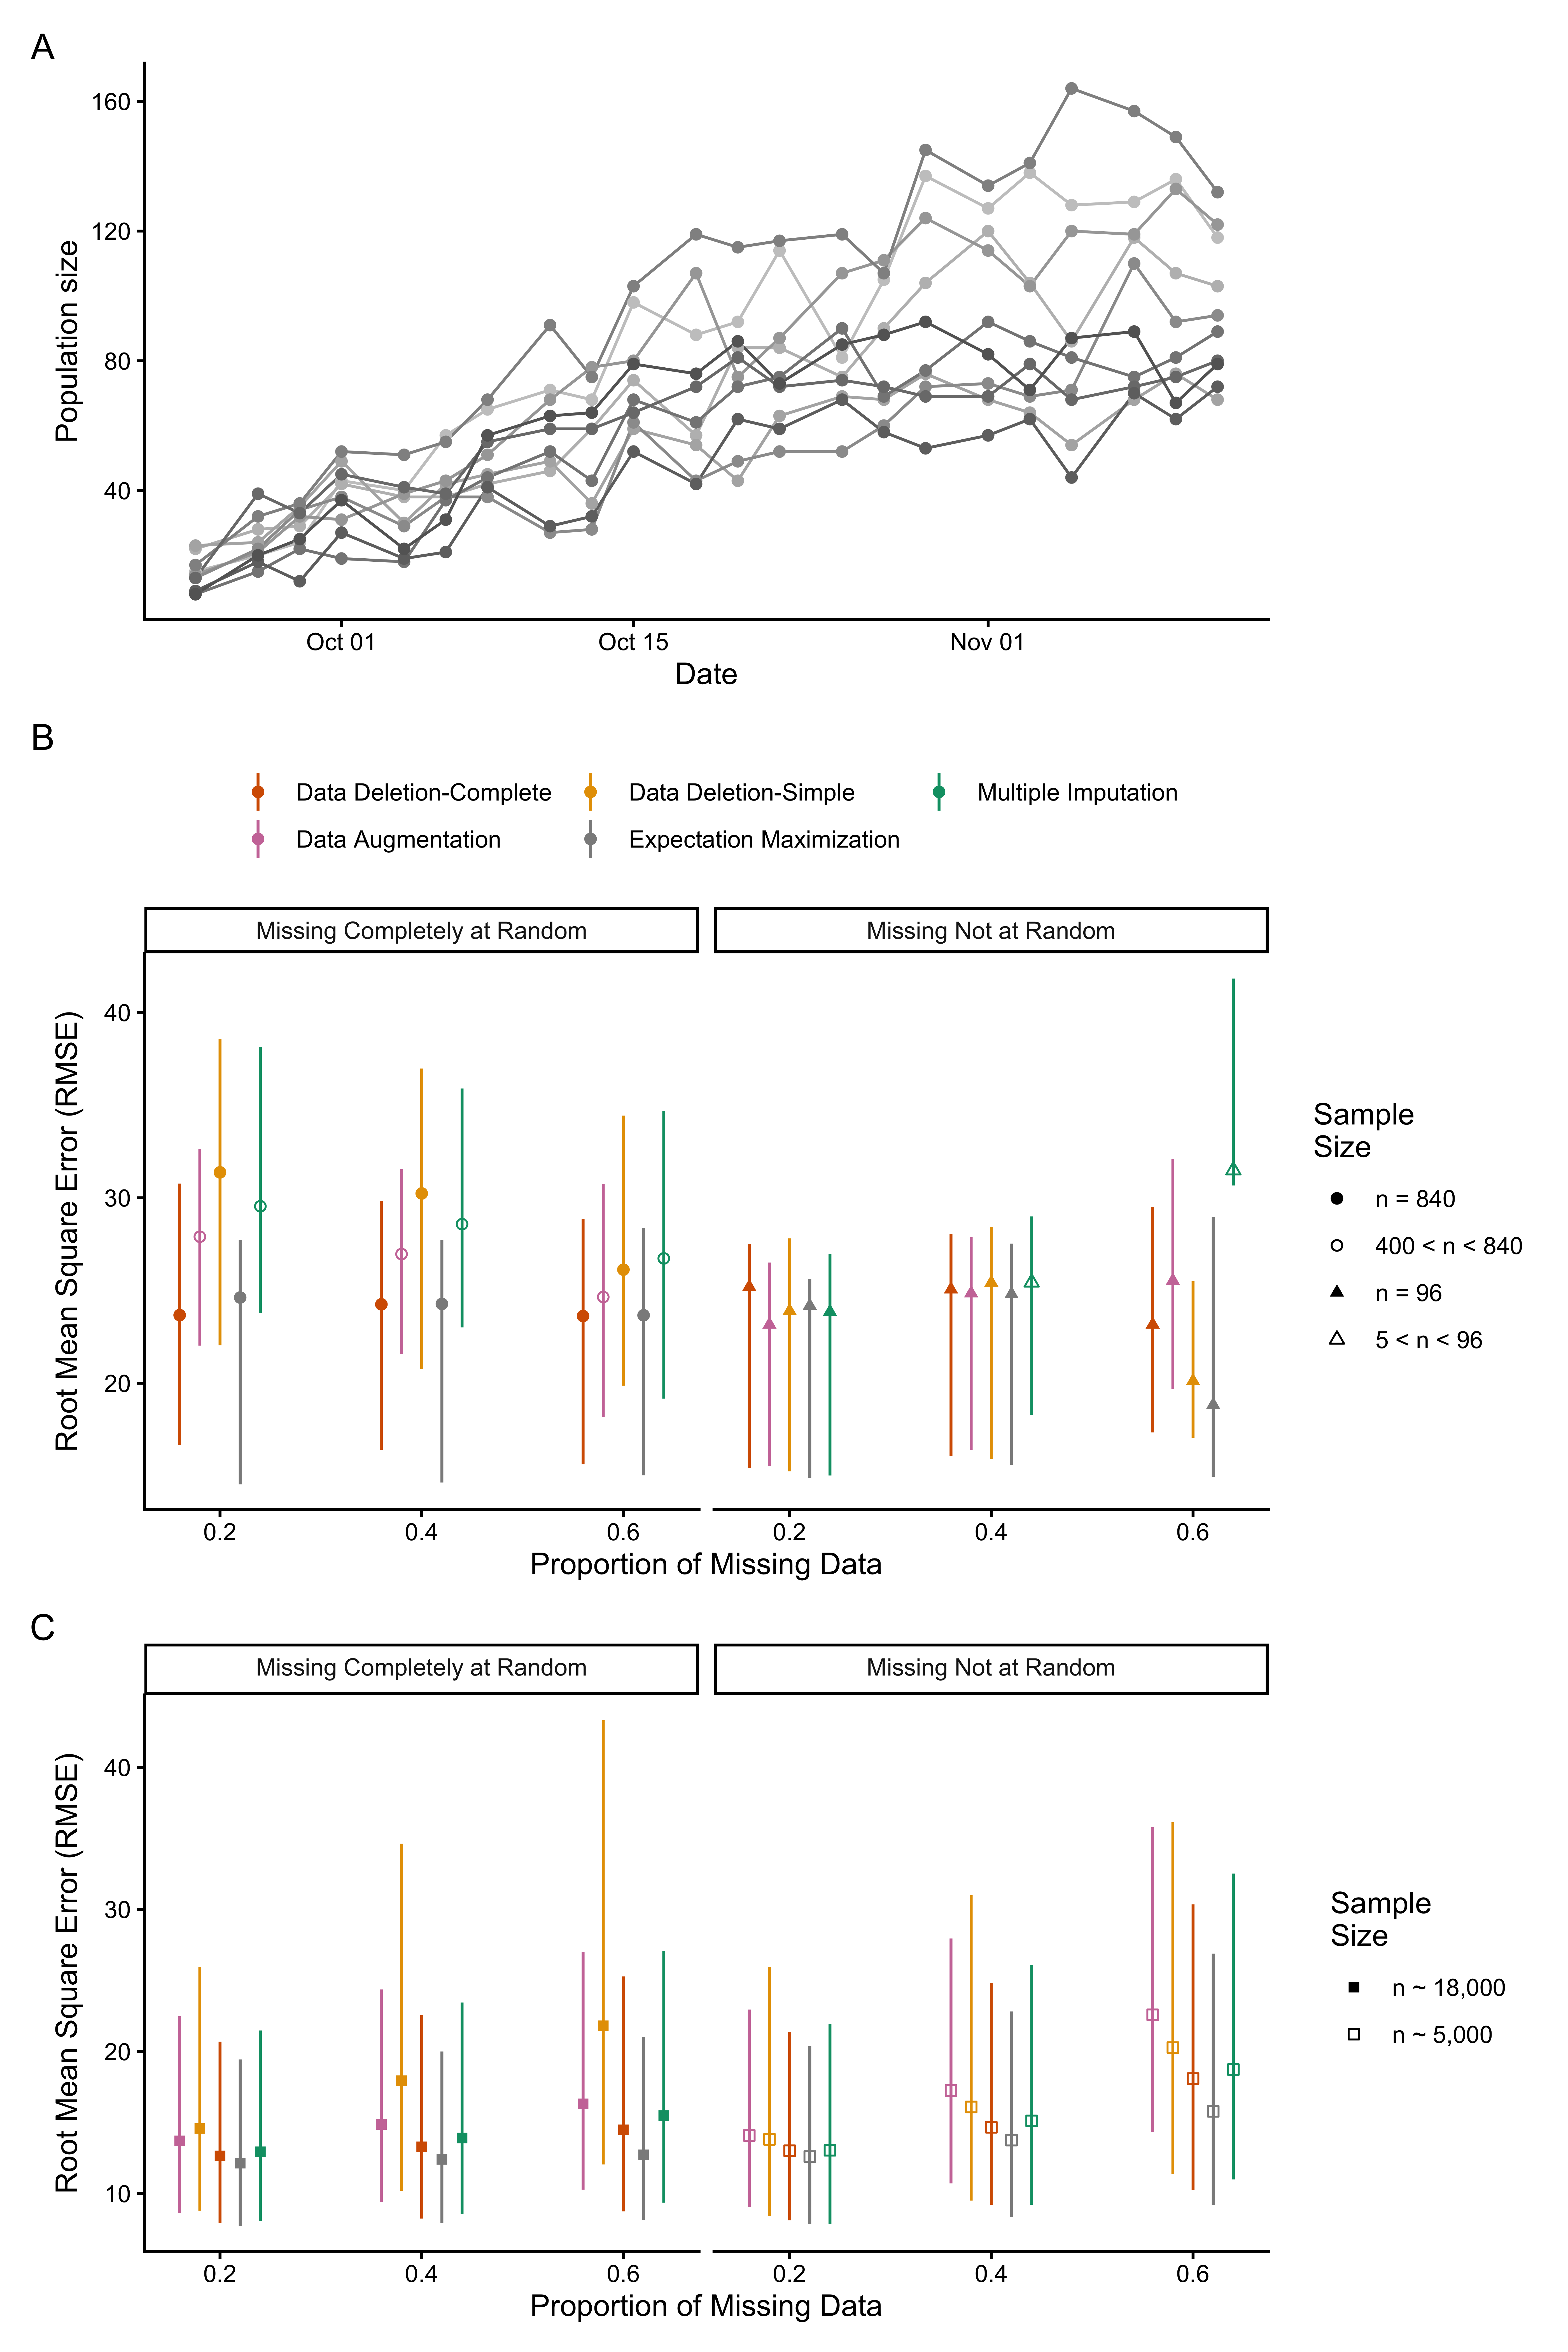
\includegraphics[width = 0.9\textwidth]{Figures/NewFiguresForRevision/RMSE_forAllPoissData.png}
    %DIF > {Figures/MockedUpFigures/RMSE_pois_combined.png}
    \DIFaddendFL \caption{}
    \label{fig:RMSE_Poiss}
\end{figure}
\clearpage

%\include{appendix}

\end{flushleft}
\end{spacing}
\end{linenumbers}
%%%%%%%%%%%%%%%%%%%%%%%%%%%%%%%
\end{document}
%%%%%%%%%%%%%%%%%%%%%%%%%%%%%%%
